\documentclass[twoside]{book}

% Packages required by doxygen
\usepackage{fixltx2e}
\usepackage{calc}
\usepackage{doxygen}
\usepackage[export]{adjustbox} % also loads graphicx
\usepackage{graphicx}
\usepackage[utf8]{inputenc}
\usepackage{makeidx}
\usepackage{multicol}
\usepackage{multirow}
\PassOptionsToPackage{warn}{textcomp}
\usepackage{textcomp}
\usepackage[nointegrals]{wasysym}
\usepackage[table]{xcolor}

% Font selection
\usepackage[T1]{fontenc}
\usepackage[scaled=.90]{helvet}
\usepackage{courier}
\usepackage{amssymb}
\usepackage{sectsty}
\renewcommand{\familydefault}{\sfdefault}
\allsectionsfont{%
  \fontseries{bc}\selectfont%
  \color{darkgray}%
}
\renewcommand{\DoxyLabelFont}{%
  \fontseries{bc}\selectfont%
  \color{darkgray}%
}
\newcommand{\+}{\discretionary{\mbox{\scriptsize$\hookleftarrow$}}{}{}}

% Page & text layout
\usepackage{geometry}
\geometry{%
  a4paper,%
  top=2.5cm,%
  bottom=2.5cm,%
  left=2.5cm,%
  right=2.5cm%
}
\tolerance=750
\hfuzz=15pt
\hbadness=750
\setlength{\emergencystretch}{15pt}
\setlength{\parindent}{0cm}
\setlength{\parskip}{3ex plus 2ex minus 2ex}
\makeatletter
\renewcommand{\paragraph}{%
  \@startsection{paragraph}{4}{0ex}{-1.0ex}{1.0ex}{%
    \normalfont\normalsize\bfseries\SS@parafont%
  }%
}
\renewcommand{\subparagraph}{%
  \@startsection{subparagraph}{5}{0ex}{-1.0ex}{1.0ex}{%
    \normalfont\normalsize\bfseries\SS@subparafont%
  }%
}
\makeatother

% Headers & footers
\usepackage{fancyhdr}
\pagestyle{fancyplain}
\fancyhead[LE]{\fancyplain{}{\bfseries\thepage}}
\fancyhead[CE]{\fancyplain{}{}}
\fancyhead[RE]{\fancyplain{}{\bfseries\leftmark}}
\fancyhead[LO]{\fancyplain{}{\bfseries\rightmark}}
\fancyhead[CO]{\fancyplain{}{}}
\fancyhead[RO]{\fancyplain{}{\bfseries\thepage}}
\fancyfoot[LE]{\fancyplain{}{}}
\fancyfoot[CE]{\fancyplain{}{}}
\fancyfoot[RE]{\fancyplain{}{\bfseries\scriptsize Generated by Doxygen }}
\fancyfoot[LO]{\fancyplain{}{\bfseries\scriptsize Generated by Doxygen }}
\fancyfoot[CO]{\fancyplain{}{}}
\fancyfoot[RO]{\fancyplain{}{}}
\renewcommand{\footrulewidth}{0.4pt}
\renewcommand{\chaptermark}[1]{%
  \markboth{#1}{}%
}
\renewcommand{\sectionmark}[1]{%
  \markright{\thesection\ #1}%
}

% Indices & bibliography
\usepackage{natbib}
\usepackage[titles]{tocloft}
\setcounter{tocdepth}{3}
\setcounter{secnumdepth}{5}
\makeindex

% Hyperlinks (required, but should be loaded last)
\usepackage{ifpdf}
\ifpdf
  \usepackage[pdftex,pagebackref=true]{hyperref}
\else
  \usepackage[ps2pdf,pagebackref=true]{hyperref}
\fi
\hypersetup{%
  colorlinks=true,%
  linkcolor=blue,%
  citecolor=blue,%
  unicode%
}

% Custom commands
\newcommand{\clearemptydoublepage}{%
  \newpage{\pagestyle{empty}\cleardoublepage}%
}

\usepackage{caption}
\captionsetup{labelsep=space,justification=centering,font={bf},singlelinecheck=off,skip=4pt,position=top}

%===== C O N T E N T S =====

\begin{document}

% Titlepage & ToC
\hypersetup{pageanchor=false,
             bookmarksnumbered=true,
             pdfencoding=unicode
            }
\pagenumbering{alph}
\begin{titlepage}
\vspace*{7cm}
\begin{center}%
{\Large Arkav\+Quarium }\\
\vspace*{1cm}
{\large Generated by Doxygen 1.8.14}\\
\end{center}
\end{titlepage}
\clearemptydoublepage
\pagenumbering{roman}
\tableofcontents
\clearemptydoublepage
\pagenumbering{arabic}
\hypersetup{pageanchor=true}

%--- Begin generated contents ---
\chapter{Hierarchical Index}
\section{Class Hierarchy}
This inheritance list is sorted roughly, but not completely, alphabetically\+:\begin{DoxyCompactList}
\item \contentsline{section}{Akuarium}{\pageref{class_akuarium}}{}
\item \contentsline{section}{Coin\+Spit}{\pageref{class_coin_spit}}{}
\begin{DoxyCompactList}
\item \contentsline{section}{Ikan}{\pageref{class_ikan}}{}
\begin{DoxyCompactList}
\item \contentsline{section}{Guppy}{\pageref{class_guppy}}{}
\item \contentsline{section}{Piranha}{\pageref{class_piranha}}{}
\end{DoxyCompactList}
\end{DoxyCompactList}
\item \contentsline{section}{List$<$ T $>$}{\pageref{class_list}}{}
\item \contentsline{section}{List$<$ Coin $>$}{\pageref{class_list}}{}
\item \contentsline{section}{List$<$ Guppy $>$}{\pageref{class_list}}{}
\item \contentsline{section}{List$<$ Makanan $>$}{\pageref{class_list}}{}
\item \contentsline{section}{List$<$ Piranha $>$}{\pageref{class_list}}{}
\item \contentsline{section}{Position}{\pageref{class_position}}{}
\begin{DoxyCompactList}
\item \contentsline{section}{Coin}{\pageref{class_coin}}{}
\item \contentsline{section}{Ikan}{\pageref{class_ikan}}{}
\item \contentsline{section}{Makanan}{\pageref{class_makanan}}{}
\item \contentsline{section}{Snail}{\pageref{class_snail}}{}
\end{DoxyCompactList}
\end{DoxyCompactList}

\chapter{Class Index}
\section{Class List}
Here are the classes, structs, unions and interfaces with brief descriptions\+:\begin{DoxyCompactList}
\item\contentsline{section}{\mbox{\hyperlink{class_akuarium}{Akuarium}} }{\pageref{class_akuarium}}{}
\item\contentsline{section}{\mbox{\hyperlink{class_coin}{Coin}} }{\pageref{class_coin}}{}
\item\contentsline{section}{\mbox{\hyperlink{class_coin_spit}{Coin\+Spit}} }{\pageref{class_coin_spit}}{}
\item\contentsline{section}{\mbox{\hyperlink{class_guppy}{Guppy}} }{\pageref{class_guppy}}{}
\item\contentsline{section}{\mbox{\hyperlink{class_ikan}{Ikan}} }{\pageref{class_ikan}}{}
\item\contentsline{section}{\mbox{\hyperlink{class_list}{List$<$ T $>$}} }{\pageref{class_list}}{}
\item\contentsline{section}{\mbox{\hyperlink{class_makanan}{Makanan}} }{\pageref{class_makanan}}{}
\item\contentsline{section}{\mbox{\hyperlink{class_piranha}{Piranha}} }{\pageref{class_piranha}}{}
\item\contentsline{section}{\mbox{\hyperlink{class_position}{Position}} }{\pageref{class_position}}{}
\item\contentsline{section}{\mbox{\hyperlink{class_snail}{Snail}} }{\pageref{class_snail}}{}
\end{DoxyCompactList}

\chapter{File Index}
\section{File List}
Here is a list of all files with brief descriptions\+:\begin{DoxyCompactList}
\item\contentsline{section}{\mbox{\hyperlink{main_8cpp}{main.\+cpp}} }{\pageref{main_8cpp}}{}
\item\contentsline{section}{headers/\mbox{\hyperlink{_akuarium_8hpp}{Akuarium.\+hpp}} }{\pageref{_akuarium_8hpp}}{}
\item\contentsline{section}{headers/\mbox{\hyperlink{_coin_8hpp}{Coin.\+hpp}} }{\pageref{_coin_8hpp}}{}
\item\contentsline{section}{headers/\mbox{\hyperlink{_coin_spit_8hpp}{Coin\+Spit.\+hpp}} }{\pageref{_coin_spit_8hpp}}{}
\item\contentsline{section}{headers/\mbox{\hyperlink{_guppy_8hpp}{Guppy.\+hpp}} }{\pageref{_guppy_8hpp}}{}
\item\contentsline{section}{headers/\mbox{\hyperlink{_ikan_8hpp}{Ikan.\+hpp}} }{\pageref{_ikan_8hpp}}{}
\item\contentsline{section}{headers/\mbox{\hyperlink{_list_8hpp}{List.\+hpp}} }{\pageref{_list_8hpp}}{}
\item\contentsline{section}{headers/\mbox{\hyperlink{_makanan_8hpp}{Makanan.\+hpp}} }{\pageref{_makanan_8hpp}}{}
\item\contentsline{section}{headers/\mbox{\hyperlink{oop_8hpp}{oop.\+hpp}} }{\pageref{oop_8hpp}}{}
\item\contentsline{section}{headers/\mbox{\hyperlink{_piranha_8hpp}{Piranha.\+hpp}} }{\pageref{_piranha_8hpp}}{}
\item\contentsline{section}{headers/\mbox{\hyperlink{_position_8hpp}{Position.\+hpp}} }{\pageref{_position_8hpp}}{}
\item\contentsline{section}{headers/\mbox{\hyperlink{_snail_8hpp}{Snail.\+hpp}} }{\pageref{_snail_8hpp}}{}
\item\contentsline{section}{src/\mbox{\hyperlink{_akuarium_8cpp}{Akuarium.\+cpp}} }{\pageref{_akuarium_8cpp}}{}
\item\contentsline{section}{src/\mbox{\hyperlink{_coin_8cpp}{Coin.\+cpp}} }{\pageref{_coin_8cpp}}{}
\item\contentsline{section}{src/\mbox{\hyperlink{_guppy_8cpp}{Guppy.\+cpp}} }{\pageref{_guppy_8cpp}}{}
\item\contentsline{section}{src/\mbox{\hyperlink{_ikan_8cpp}{Ikan.\+cpp}} }{\pageref{_ikan_8cpp}}{}
\item\contentsline{section}{src/\mbox{\hyperlink{_makanan_8cpp}{Makanan.\+cpp}} }{\pageref{_makanan_8cpp}}{}
\item\contentsline{section}{src/\mbox{\hyperlink{oop_8cpp}{oop.\+cpp}} }{\pageref{oop_8cpp}}{}
\item\contentsline{section}{src/\mbox{\hyperlink{_piranha_8cpp}{Piranha.\+cpp}} }{\pageref{_piranha_8cpp}}{}
\item\contentsline{section}{src/\mbox{\hyperlink{_position_8cpp}{Position.\+cpp}} }{\pageref{_position_8cpp}}{}
\item\contentsline{section}{src/\mbox{\hyperlink{_snail_8cpp}{Snail.\+cpp}} }{\pageref{_snail_8cpp}}{}
\item\contentsline{section}{test\+\_\+driver/\+Coin/\mbox{\hyperlink{main__coin_8cpp}{main\+\_\+coin.\+cpp}} }{\pageref{main__coin_8cpp}}{}
\item\contentsline{section}{test\+\_\+driver/\+Guppy/\mbox{\hyperlink{main__guppy_8cpp}{main\+\_\+guppy.\+cpp}} }{\pageref{main__guppy_8cpp}}{}
\item\contentsline{section}{test\+\_\+driver/\+List/\mbox{\hyperlink{main__list_8cpp}{main\+\_\+list.\+cpp}} }{\pageref{main__list_8cpp}}{}
\item\contentsline{section}{test\+\_\+driver/\+Makanan/\mbox{\hyperlink{main__makanan_8cpp}{main\+\_\+makanan.\+cpp}} }{\pageref{main__makanan_8cpp}}{}
\item\contentsline{section}{test\+\_\+driver/\+Piranha/\mbox{\hyperlink{_piranha__test_8cpp}{Piranha\+\_\+test.\+cpp}} }{\pageref{_piranha__test_8cpp}}{}
\item\contentsline{section}{test\+\_\+driver/\+Position/\mbox{\hyperlink{main__position_8cpp}{main\+\_\+position.\+cpp}} }{\pageref{main__position_8cpp}}{}
\end{DoxyCompactList}

\chapter{Class Documentation}
\hypertarget{class_akuarium}{}\section{Akuarium Class Reference}
\label{class_akuarium}\index{Akuarium@{Akuarium}}


{\ttfamily \#include $<$Akuarium.\+hpp$>$}



Collaboration diagram for Akuarium\+:
\nopagebreak
\begin{figure}[H]
\begin{center}
\leavevmode
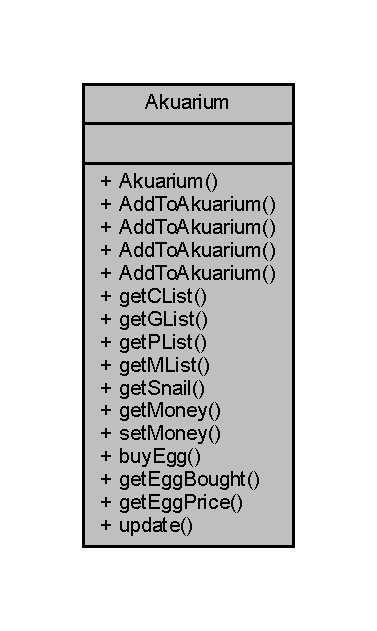
\includegraphics[width=181pt]{class_akuarium__coll__graph}
\end{center}
\end{figure}
\subsection*{Public Member Functions}
\begin{DoxyCompactItemize}
\item 
\mbox{\hyperlink{class_akuarium_a09356fa0405a5c8db4b048665456e1ce}{Akuarium}} (int x\+Max, int y\+Max)
\item 
void \mbox{\hyperlink{class_akuarium_acd7f2fd40ce2ca063c3ddfacf1a84ea3}{Add\+To\+Akuarium}} (\mbox{\hyperlink{class_guppy}{Guppy}} $\ast$G)
\item 
void \mbox{\hyperlink{class_akuarium_a167b796ece0cdd537c5c6624ed15760c}{Add\+To\+Akuarium}} (\mbox{\hyperlink{class_piranha}{Piranha}} $\ast$P)
\item 
void \mbox{\hyperlink{class_akuarium_a1f4f9363a6d7293e24768b6f70ee2eae}{Add\+To\+Akuarium}} (\mbox{\hyperlink{class_coin}{Coin}} $\ast$C)
\item 
void \mbox{\hyperlink{class_akuarium_a83bb5abf33474615c762124429a350be}{Add\+To\+Akuarium}} (\mbox{\hyperlink{class_makanan}{Makanan}} $\ast$M)
\item 
\mbox{\hyperlink{class_list}{List}}$<$ \mbox{\hyperlink{class_coin}{Coin}} $>$ $\ast$ \mbox{\hyperlink{class_akuarium_a8eebf8e6e312dee21e4d790de5e6f614}{get\+C\+List}} ()
\item 
\mbox{\hyperlink{class_list}{List}}$<$ \mbox{\hyperlink{class_guppy}{Guppy}} $>$ $\ast$ \mbox{\hyperlink{class_akuarium_aea95fa5feed9d17dd8cee6a716413222}{get\+G\+List}} ()
\item 
\mbox{\hyperlink{class_list}{List}}$<$ \mbox{\hyperlink{class_piranha}{Piranha}} $>$ $\ast$ \mbox{\hyperlink{class_akuarium_ad6e04ad77928d85f6739b76c9efaaa67}{get\+P\+List}} ()
\item 
\mbox{\hyperlink{class_list}{List}}$<$ \mbox{\hyperlink{class_makanan}{Makanan}} $>$ $\ast$ \mbox{\hyperlink{class_akuarium_aceb32b9271d3de1c5383151d68a16cdb}{get\+M\+List}} ()
\item 
\mbox{\hyperlink{class_snail}{Snail}} $\ast$ \mbox{\hyperlink{class_akuarium_a846c24525e4bec5b355e34924d8a5784}{get\+Snail}} ()
\item 
int \mbox{\hyperlink{class_akuarium_a641dd24ff82bc9eab91c119cef4ac06c}{get\+Money}} ()
\item 
void \mbox{\hyperlink{class_akuarium_a6be2d50883019668db71ef5128851202}{set\+Money}} (int money)
\item 
int \mbox{\hyperlink{class_akuarium_ab68614c24c06e011b93cc5d03103f352}{buy\+Egg}} ()
\item 
int \mbox{\hyperlink{class_akuarium_ad5c60aa9ac76b1af2de9ed50765ef9cf}{get\+Egg\+Bought}} ()
\item 
const int \mbox{\hyperlink{class_akuarium_a45b387e510e5a938017908a63d22283c}{get\+Egg\+Price}} ()
\item 
void \mbox{\hyperlink{class_akuarium_af7c9d5e5b90bd3c0cef6e91777bb3978}{update}} (double sec\+\_\+since\+\_\+last)
\end{DoxyCompactItemize}


\subsection{Constructor \& Destructor Documentation}
\mbox{\Hypertarget{class_akuarium_a09356fa0405a5c8db4b048665456e1ce}\label{class_akuarium_a09356fa0405a5c8db4b048665456e1ce}} 
\index{Akuarium@{Akuarium}!Akuarium@{Akuarium}}
\index{Akuarium@{Akuarium}!Akuarium@{Akuarium}}
\subsubsection{\texorpdfstring{Akuarium()}{Akuarium()}}
{\footnotesize\ttfamily Akuarium\+::\+Akuarium (\begin{DoxyParamCaption}\item[{int}]{x\+Max,  }\item[{int}]{y\+Max }\end{DoxyParamCaption})}



\subsection{Member Function Documentation}
\mbox{\Hypertarget{class_akuarium_acd7f2fd40ce2ca063c3ddfacf1a84ea3}\label{class_akuarium_acd7f2fd40ce2ca063c3ddfacf1a84ea3}} 
\index{Akuarium@{Akuarium}!Add\+To\+Akuarium@{Add\+To\+Akuarium}}
\index{Add\+To\+Akuarium@{Add\+To\+Akuarium}!Akuarium@{Akuarium}}
\subsubsection{\texorpdfstring{Add\+To\+Akuarium()}{AddToAkuarium()}\hspace{0.1cm}{\footnotesize\ttfamily [1/4]}}
{\footnotesize\ttfamily void Akuarium\+::\+Add\+To\+Akuarium (\begin{DoxyParamCaption}\item[{\mbox{\hyperlink{class_guppy}{Guppy}} $\ast$}]{G }\end{DoxyParamCaption})}

\mbox{\Hypertarget{class_akuarium_a167b796ece0cdd537c5c6624ed15760c}\label{class_akuarium_a167b796ece0cdd537c5c6624ed15760c}} 
\index{Akuarium@{Akuarium}!Add\+To\+Akuarium@{Add\+To\+Akuarium}}
\index{Add\+To\+Akuarium@{Add\+To\+Akuarium}!Akuarium@{Akuarium}}
\subsubsection{\texorpdfstring{Add\+To\+Akuarium()}{AddToAkuarium()}\hspace{0.1cm}{\footnotesize\ttfamily [2/4]}}
{\footnotesize\ttfamily void Akuarium\+::\+Add\+To\+Akuarium (\begin{DoxyParamCaption}\item[{\mbox{\hyperlink{class_piranha}{Piranha}} $\ast$}]{P }\end{DoxyParamCaption})}

\mbox{\Hypertarget{class_akuarium_a1f4f9363a6d7293e24768b6f70ee2eae}\label{class_akuarium_a1f4f9363a6d7293e24768b6f70ee2eae}} 
\index{Akuarium@{Akuarium}!Add\+To\+Akuarium@{Add\+To\+Akuarium}}
\index{Add\+To\+Akuarium@{Add\+To\+Akuarium}!Akuarium@{Akuarium}}
\subsubsection{\texorpdfstring{Add\+To\+Akuarium()}{AddToAkuarium()}\hspace{0.1cm}{\footnotesize\ttfamily [3/4]}}
{\footnotesize\ttfamily void Akuarium\+::\+Add\+To\+Akuarium (\begin{DoxyParamCaption}\item[{\mbox{\hyperlink{class_coin}{Coin}} $\ast$}]{C }\end{DoxyParamCaption})}

\mbox{\Hypertarget{class_akuarium_a83bb5abf33474615c762124429a350be}\label{class_akuarium_a83bb5abf33474615c762124429a350be}} 
\index{Akuarium@{Akuarium}!Add\+To\+Akuarium@{Add\+To\+Akuarium}}
\index{Add\+To\+Akuarium@{Add\+To\+Akuarium}!Akuarium@{Akuarium}}
\subsubsection{\texorpdfstring{Add\+To\+Akuarium()}{AddToAkuarium()}\hspace{0.1cm}{\footnotesize\ttfamily [4/4]}}
{\footnotesize\ttfamily void Akuarium\+::\+Add\+To\+Akuarium (\begin{DoxyParamCaption}\item[{\mbox{\hyperlink{class_makanan}{Makanan}} $\ast$}]{M }\end{DoxyParamCaption})}

\mbox{\Hypertarget{class_akuarium_ab68614c24c06e011b93cc5d03103f352}\label{class_akuarium_ab68614c24c06e011b93cc5d03103f352}} 
\index{Akuarium@{Akuarium}!buy\+Egg@{buy\+Egg}}
\index{buy\+Egg@{buy\+Egg}!Akuarium@{Akuarium}}
\subsubsection{\texorpdfstring{buy\+Egg()}{buyEgg()}}
{\footnotesize\ttfamily int Akuarium\+::buy\+Egg (\begin{DoxyParamCaption}{ }\end{DoxyParamCaption})}

\mbox{\Hypertarget{class_akuarium_a8eebf8e6e312dee21e4d790de5e6f614}\label{class_akuarium_a8eebf8e6e312dee21e4d790de5e6f614}} 
\index{Akuarium@{Akuarium}!get\+C\+List@{get\+C\+List}}
\index{get\+C\+List@{get\+C\+List}!Akuarium@{Akuarium}}
\subsubsection{\texorpdfstring{get\+C\+List()}{getCList()}}
{\footnotesize\ttfamily \mbox{\hyperlink{class_list}{List}}$<$ \mbox{\hyperlink{class_coin}{Coin}} $>$ $\ast$ Akuarium\+::get\+C\+List (\begin{DoxyParamCaption}{ }\end{DoxyParamCaption})}

\mbox{\Hypertarget{class_akuarium_ad5c60aa9ac76b1af2de9ed50765ef9cf}\label{class_akuarium_ad5c60aa9ac76b1af2de9ed50765ef9cf}} 
\index{Akuarium@{Akuarium}!get\+Egg\+Bought@{get\+Egg\+Bought}}
\index{get\+Egg\+Bought@{get\+Egg\+Bought}!Akuarium@{Akuarium}}
\subsubsection{\texorpdfstring{get\+Egg\+Bought()}{getEggBought()}}
{\footnotesize\ttfamily int Akuarium\+::get\+Egg\+Bought (\begin{DoxyParamCaption}{ }\end{DoxyParamCaption})}

\mbox{\Hypertarget{class_akuarium_a45b387e510e5a938017908a63d22283c}\label{class_akuarium_a45b387e510e5a938017908a63d22283c}} 
\index{Akuarium@{Akuarium}!get\+Egg\+Price@{get\+Egg\+Price}}
\index{get\+Egg\+Price@{get\+Egg\+Price}!Akuarium@{Akuarium}}
\subsubsection{\texorpdfstring{get\+Egg\+Price()}{getEggPrice()}}
{\footnotesize\ttfamily const int Akuarium\+::get\+Egg\+Price (\begin{DoxyParamCaption}{ }\end{DoxyParamCaption})}

\mbox{\Hypertarget{class_akuarium_aea95fa5feed9d17dd8cee6a716413222}\label{class_akuarium_aea95fa5feed9d17dd8cee6a716413222}} 
\index{Akuarium@{Akuarium}!get\+G\+List@{get\+G\+List}}
\index{get\+G\+List@{get\+G\+List}!Akuarium@{Akuarium}}
\subsubsection{\texorpdfstring{get\+G\+List()}{getGList()}}
{\footnotesize\ttfamily \mbox{\hyperlink{class_list}{List}}$<$ \mbox{\hyperlink{class_guppy}{Guppy}} $>$ $\ast$ Akuarium\+::get\+G\+List (\begin{DoxyParamCaption}{ }\end{DoxyParamCaption})}

\mbox{\Hypertarget{class_akuarium_aceb32b9271d3de1c5383151d68a16cdb}\label{class_akuarium_aceb32b9271d3de1c5383151d68a16cdb}} 
\index{Akuarium@{Akuarium}!get\+M\+List@{get\+M\+List}}
\index{get\+M\+List@{get\+M\+List}!Akuarium@{Akuarium}}
\subsubsection{\texorpdfstring{get\+M\+List()}{getMList()}}
{\footnotesize\ttfamily \mbox{\hyperlink{class_list}{List}}$<$ \mbox{\hyperlink{class_makanan}{Makanan}} $>$ $\ast$ Akuarium\+::get\+M\+List (\begin{DoxyParamCaption}{ }\end{DoxyParamCaption})}

\mbox{\Hypertarget{class_akuarium_a641dd24ff82bc9eab91c119cef4ac06c}\label{class_akuarium_a641dd24ff82bc9eab91c119cef4ac06c}} 
\index{Akuarium@{Akuarium}!get\+Money@{get\+Money}}
\index{get\+Money@{get\+Money}!Akuarium@{Akuarium}}
\subsubsection{\texorpdfstring{get\+Money()}{getMoney()}}
{\footnotesize\ttfamily int Akuarium\+::get\+Money (\begin{DoxyParamCaption}{ }\end{DoxyParamCaption})}

\mbox{\Hypertarget{class_akuarium_ad6e04ad77928d85f6739b76c9efaaa67}\label{class_akuarium_ad6e04ad77928d85f6739b76c9efaaa67}} 
\index{Akuarium@{Akuarium}!get\+P\+List@{get\+P\+List}}
\index{get\+P\+List@{get\+P\+List}!Akuarium@{Akuarium}}
\subsubsection{\texorpdfstring{get\+P\+List()}{getPList()}}
{\footnotesize\ttfamily \mbox{\hyperlink{class_list}{List}}$<$ \mbox{\hyperlink{class_piranha}{Piranha}} $>$ $\ast$ Akuarium\+::get\+P\+List (\begin{DoxyParamCaption}{ }\end{DoxyParamCaption})}

\mbox{\Hypertarget{class_akuarium_a846c24525e4bec5b355e34924d8a5784}\label{class_akuarium_a846c24525e4bec5b355e34924d8a5784}} 
\index{Akuarium@{Akuarium}!get\+Snail@{get\+Snail}}
\index{get\+Snail@{get\+Snail}!Akuarium@{Akuarium}}
\subsubsection{\texorpdfstring{get\+Snail()}{getSnail()}}
{\footnotesize\ttfamily \mbox{\hyperlink{class_snail}{Snail}} $\ast$ Akuarium\+::get\+Snail (\begin{DoxyParamCaption}{ }\end{DoxyParamCaption})}

\mbox{\Hypertarget{class_akuarium_a6be2d50883019668db71ef5128851202}\label{class_akuarium_a6be2d50883019668db71ef5128851202}} 
\index{Akuarium@{Akuarium}!set\+Money@{set\+Money}}
\index{set\+Money@{set\+Money}!Akuarium@{Akuarium}}
\subsubsection{\texorpdfstring{set\+Money()}{setMoney()}}
{\footnotesize\ttfamily void Akuarium\+::set\+Money (\begin{DoxyParamCaption}\item[{int}]{money }\end{DoxyParamCaption})}

\mbox{\Hypertarget{class_akuarium_af7c9d5e5b90bd3c0cef6e91777bb3978}\label{class_akuarium_af7c9d5e5b90bd3c0cef6e91777bb3978}} 
\index{Akuarium@{Akuarium}!update@{update}}
\index{update@{update}!Akuarium@{Akuarium}}
\subsubsection{\texorpdfstring{update()}{update()}}
{\footnotesize\ttfamily void Akuarium\+::update (\begin{DoxyParamCaption}\item[{double}]{sec\+\_\+since\+\_\+last }\end{DoxyParamCaption})}



The documentation for this class was generated from the following files\+:\begin{DoxyCompactItemize}
\item 
C\+:/\+Users/user/\+Desktop/technical stuff/cpp/\+Tubes O\+O\+P/\+Main Folder/headers/\mbox{\hyperlink{_akuarium_8hpp}{Akuarium.\+hpp}}\item 
C\+:/\+Users/user/\+Desktop/technical stuff/cpp/\+Tubes O\+O\+P/\+Main Folder/src/\mbox{\hyperlink{_akuarium_8cpp}{Akuarium.\+cpp}}\end{DoxyCompactItemize}

\hypertarget{class_coin}{}\section{Coin Class Reference}
\label{class_coin}\index{Coin@{Coin}}


{\ttfamily \#include $<$Coin.\+hpp$>$}



Inheritance diagram for Coin\+:
\nopagebreak
\begin{figure}[H]
\begin{center}
\leavevmode
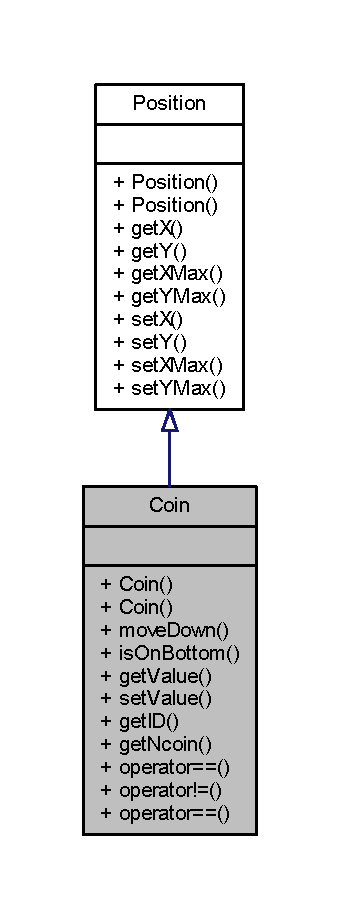
\includegraphics[width=163pt]{class_coin__inherit__graph}
\end{center}
\end{figure}


Collaboration diagram for Coin\+:
\nopagebreak
\begin{figure}[H]
\begin{center}
\leavevmode
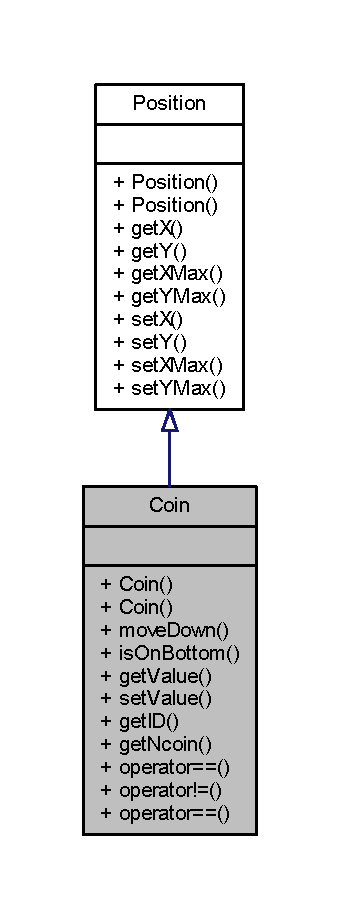
\includegraphics[width=163pt]{class_coin__coll__graph}
\end{center}
\end{figure}
\subsection*{Public Member Functions}
\begin{DoxyCompactItemize}
\item 
\mbox{\hyperlink{class_coin_a94b2130e2d3ac956ba47271ad81c64f5}{Coin}} ()
\item 
\mbox{\hyperlink{class_coin_a15165b502ff8217f0d85df18a9a30179}{Coin}} (int x, int y, int val, int xmax, int ymax)
\item 
void \mbox{\hyperlink{class_coin_af45c31b09753600787ffe0319db28298}{move\+Down}} (double sec\+\_\+since\+\_\+last)
\item 
bool \mbox{\hyperlink{class_coin_a210e01a3e058d02076fe3b138785703b}{is\+On\+Bottom}} () const
\item 
int \mbox{\hyperlink{class_coin_a53c8bf65afdde1422cfda51d753d74b7}{get\+Value}} () const
\item 
void \mbox{\hyperlink{class_coin_a87813c8eef4d59ef8136b0cc651a80de}{set\+Value}} (int val)
\item 
int \mbox{\hyperlink{class_coin_ad0a324384f93ebe7ef0b9786f1ceaae4}{get\+ID}} ()
\item 
int \mbox{\hyperlink{class_coin_a218706448b94dbdf9299603f2195c064}{get\+Ncoin}} ()
\item 
bool \mbox{\hyperlink{class_coin_ae12c00f84a81afbb7edb2aa3b9842683}{operator==}} (const \mbox{\hyperlink{class_coin}{Coin}} \&C)
\item 
bool \mbox{\hyperlink{class_coin_a67152a3b3ca628c5a122bea522a80b6e}{operator!=}} (const \mbox{\hyperlink{class_coin}{Coin}} \&C)
\item 
bool \mbox{\hyperlink{class_coin_a20ef59bfc867081e452d38daded77e08}{operator==}} (std\+::nullptr\+\_\+t n)
\end{DoxyCompactItemize}


\subsection{Constructor \& Destructor Documentation}
\mbox{\Hypertarget{class_coin_a94b2130e2d3ac956ba47271ad81c64f5}\label{class_coin_a94b2130e2d3ac956ba47271ad81c64f5}} 
\index{Coin@{Coin}!Coin@{Coin}}
\index{Coin@{Coin}!Coin@{Coin}}
\subsubsection{\texorpdfstring{Coin()}{Coin()}\hspace{0.1cm}{\footnotesize\ttfamily [1/2]}}
{\footnotesize\ttfamily Coin\+::\+Coin (\begin{DoxyParamCaption}{ }\end{DoxyParamCaption})}

\mbox{\Hypertarget{class_coin_a15165b502ff8217f0d85df18a9a30179}\label{class_coin_a15165b502ff8217f0d85df18a9a30179}} 
\index{Coin@{Coin}!Coin@{Coin}}
\index{Coin@{Coin}!Coin@{Coin}}
\subsubsection{\texorpdfstring{Coin()}{Coin()}\hspace{0.1cm}{\footnotesize\ttfamily [2/2]}}
{\footnotesize\ttfamily Coin\+::\+Coin (\begin{DoxyParamCaption}\item[{int}]{x,  }\item[{int}]{y,  }\item[{int}]{val,  }\item[{int}]{xmax,  }\item[{int}]{ymax }\end{DoxyParamCaption})}



\subsection{Member Function Documentation}
\mbox{\Hypertarget{class_coin_ad0a324384f93ebe7ef0b9786f1ceaae4}\label{class_coin_ad0a324384f93ebe7ef0b9786f1ceaae4}} 
\index{Coin@{Coin}!get\+ID@{get\+ID}}
\index{get\+ID@{get\+ID}!Coin@{Coin}}
\subsubsection{\texorpdfstring{get\+I\+D()}{getID()}}
{\footnotesize\ttfamily int Coin\+::get\+ID (\begin{DoxyParamCaption}{ }\end{DoxyParamCaption})}

\mbox{\Hypertarget{class_coin_a218706448b94dbdf9299603f2195c064}\label{class_coin_a218706448b94dbdf9299603f2195c064}} 
\index{Coin@{Coin}!get\+Ncoin@{get\+Ncoin}}
\index{get\+Ncoin@{get\+Ncoin}!Coin@{Coin}}
\subsubsection{\texorpdfstring{get\+Ncoin()}{getNcoin()}}
{\footnotesize\ttfamily int Coin\+::get\+Ncoin (\begin{DoxyParamCaption}{ }\end{DoxyParamCaption})}

\mbox{\Hypertarget{class_coin_a53c8bf65afdde1422cfda51d753d74b7}\label{class_coin_a53c8bf65afdde1422cfda51d753d74b7}} 
\index{Coin@{Coin}!get\+Value@{get\+Value}}
\index{get\+Value@{get\+Value}!Coin@{Coin}}
\subsubsection{\texorpdfstring{get\+Value()}{getValue()}}
{\footnotesize\ttfamily int Coin\+::get\+Value (\begin{DoxyParamCaption}{ }\end{DoxyParamCaption}) const}

\mbox{\Hypertarget{class_coin_a210e01a3e058d02076fe3b138785703b}\label{class_coin_a210e01a3e058d02076fe3b138785703b}} 
\index{Coin@{Coin}!is\+On\+Bottom@{is\+On\+Bottom}}
\index{is\+On\+Bottom@{is\+On\+Bottom}!Coin@{Coin}}
\subsubsection{\texorpdfstring{is\+On\+Bottom()}{isOnBottom()}}
{\footnotesize\ttfamily bool Coin\+::is\+On\+Bottom (\begin{DoxyParamCaption}{ }\end{DoxyParamCaption}) const}

\mbox{\Hypertarget{class_coin_af45c31b09753600787ffe0319db28298}\label{class_coin_af45c31b09753600787ffe0319db28298}} 
\index{Coin@{Coin}!move\+Down@{move\+Down}}
\index{move\+Down@{move\+Down}!Coin@{Coin}}
\subsubsection{\texorpdfstring{move\+Down()}{moveDown()}}
{\footnotesize\ttfamily void Coin\+::move\+Down (\begin{DoxyParamCaption}\item[{double}]{sec\+\_\+since\+\_\+last }\end{DoxyParamCaption})}

\mbox{\Hypertarget{class_coin_a67152a3b3ca628c5a122bea522a80b6e}\label{class_coin_a67152a3b3ca628c5a122bea522a80b6e}} 
\index{Coin@{Coin}!operator"!=@{operator"!=}}
\index{operator"!=@{operator"!=}!Coin@{Coin}}
\subsubsection{\texorpdfstring{operator"!=()}{operator!=()}}
{\footnotesize\ttfamily bool Coin\+::operator!= (\begin{DoxyParamCaption}\item[{const \mbox{\hyperlink{class_coin}{Coin}} \&}]{C }\end{DoxyParamCaption})}

\mbox{\Hypertarget{class_coin_ae12c00f84a81afbb7edb2aa3b9842683}\label{class_coin_ae12c00f84a81afbb7edb2aa3b9842683}} 
\index{Coin@{Coin}!operator==@{operator==}}
\index{operator==@{operator==}!Coin@{Coin}}
\subsubsection{\texorpdfstring{operator==()}{operator==()}\hspace{0.1cm}{\footnotesize\ttfamily [1/2]}}
{\footnotesize\ttfamily bool Coin\+::operator== (\begin{DoxyParamCaption}\item[{const \mbox{\hyperlink{class_coin}{Coin}} \&}]{C }\end{DoxyParamCaption})}

\mbox{\Hypertarget{class_coin_a20ef59bfc867081e452d38daded77e08}\label{class_coin_a20ef59bfc867081e452d38daded77e08}} 
\index{Coin@{Coin}!operator==@{operator==}}
\index{operator==@{operator==}!Coin@{Coin}}
\subsubsection{\texorpdfstring{operator==()}{operator==()}\hspace{0.1cm}{\footnotesize\ttfamily [2/2]}}
{\footnotesize\ttfamily bool Coin\+::operator== (\begin{DoxyParamCaption}\item[{std\+::nullptr\+\_\+t}]{n }\end{DoxyParamCaption})}

\mbox{\Hypertarget{class_coin_a87813c8eef4d59ef8136b0cc651a80de}\label{class_coin_a87813c8eef4d59ef8136b0cc651a80de}} 
\index{Coin@{Coin}!set\+Value@{set\+Value}}
\index{set\+Value@{set\+Value}!Coin@{Coin}}
\subsubsection{\texorpdfstring{set\+Value()}{setValue()}}
{\footnotesize\ttfamily void Coin\+::set\+Value (\begin{DoxyParamCaption}\item[{int}]{val }\end{DoxyParamCaption})}



The documentation for this class was generated from the following files\+:\begin{DoxyCompactItemize}
\item 
C\+:/\+Users/user/\+Desktop/technical stuff/cpp/\+Tubes O\+O\+P/\+Main Folder/headers/\mbox{\hyperlink{_coin_8hpp}{Coin.\+hpp}}\item 
C\+:/\+Users/user/\+Desktop/technical stuff/cpp/\+Tubes O\+O\+P/\+Main Folder/src/\mbox{\hyperlink{_coin_8cpp}{Coin.\+cpp}}\end{DoxyCompactItemize}

\hypertarget{class_coin_spit}{}\section{Coin\+Spit Class Reference}
\label{class_coin_spit}\index{Coin\+Spit@{Coin\+Spit}}


{\ttfamily \#include $<$Coin\+Spit.\+hpp$>$}



Inheritance diagram for Coin\+Spit\+:
\nopagebreak
\begin{figure}[H]
\begin{center}
\leavevmode
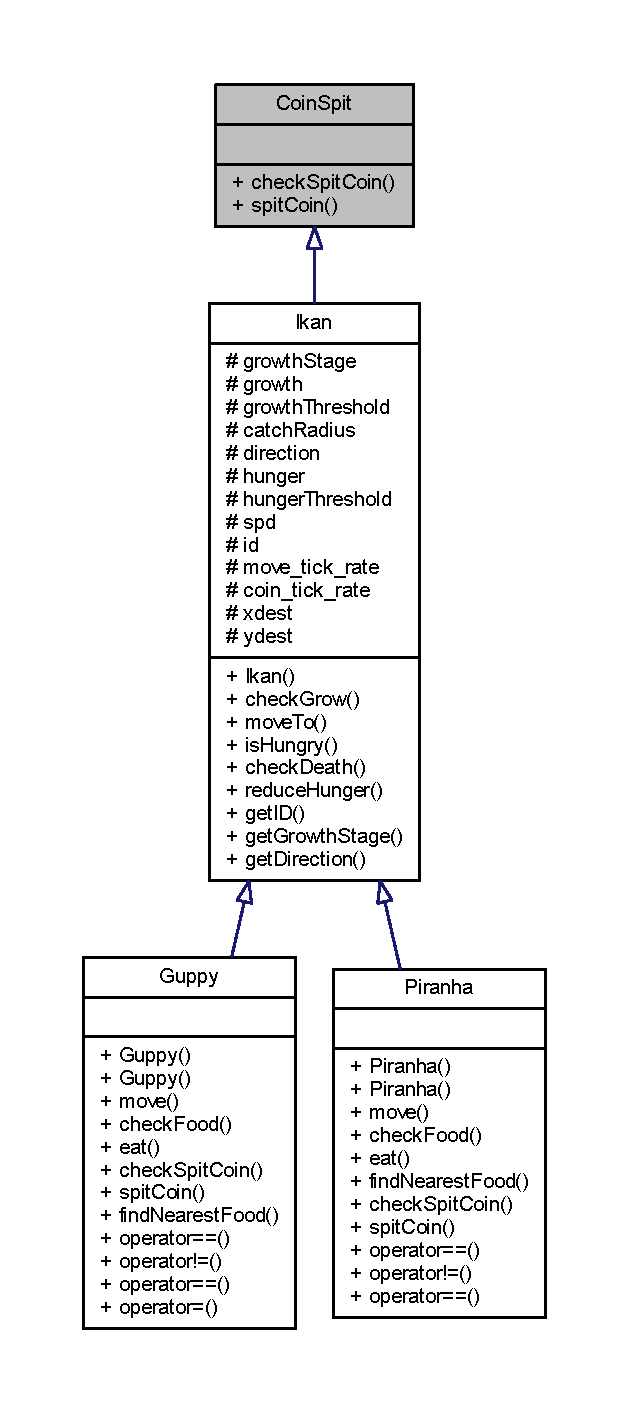
\includegraphics[height=550pt]{class_coin_spit__inherit__graph}
\end{center}
\end{figure}


Collaboration diagram for Coin\+Spit\+:
\nopagebreak
\begin{figure}[H]
\begin{center}
\leavevmode
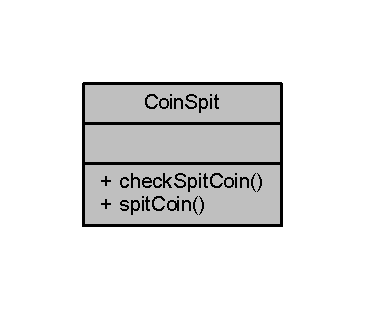
\includegraphics[width=175pt]{class_coin_spit__coll__graph}
\end{center}
\end{figure}
\subsection*{Public Member Functions}
\begin{DoxyCompactItemize}
\item 
virtual bool \mbox{\hyperlink{class_coin_spit_a9471108f825dc67a35ac1a35444b84fd}{check\+Spit\+Coin}} ()=0
\item 
virtual void \mbox{\hyperlink{class_coin_spit_a336f45a90c4b0b57017b45a5c68f12a7}{spit\+Coin}} (\mbox{\hyperlink{class_list}{List}}$<$ \mbox{\hyperlink{class_coin}{Coin}} $>$ \&Lcoin, int value)=0
\end{DoxyCompactItemize}


\subsection{Member Function Documentation}
\mbox{\Hypertarget{class_coin_spit_a9471108f825dc67a35ac1a35444b84fd}\label{class_coin_spit_a9471108f825dc67a35ac1a35444b84fd}} 
\index{Coin\+Spit@{Coin\+Spit}!check\+Spit\+Coin@{check\+Spit\+Coin}}
\index{check\+Spit\+Coin@{check\+Spit\+Coin}!Coin\+Spit@{Coin\+Spit}}
\subsubsection{\texorpdfstring{check\+Spit\+Coin()}{checkSpitCoin()}}
{\footnotesize\ttfamily virtual bool Coin\+Spit\+::check\+Spit\+Coin (\begin{DoxyParamCaption}{ }\end{DoxyParamCaption})\hspace{0.3cm}{\ttfamily [pure virtual]}}



Implemented in \mbox{\hyperlink{class_guppy_abab3975de3a054b14aa3b8e664e30b5b}{Guppy}}, and \mbox{\hyperlink{class_piranha_a9db3ab2f9933739f5744e881f9ee386e}{Piranha}}.

\mbox{\Hypertarget{class_coin_spit_a336f45a90c4b0b57017b45a5c68f12a7}\label{class_coin_spit_a336f45a90c4b0b57017b45a5c68f12a7}} 
\index{Coin\+Spit@{Coin\+Spit}!spit\+Coin@{spit\+Coin}}
\index{spit\+Coin@{spit\+Coin}!Coin\+Spit@{Coin\+Spit}}
\subsubsection{\texorpdfstring{spit\+Coin()}{spitCoin()}}
{\footnotesize\ttfamily virtual void Coin\+Spit\+::spit\+Coin (\begin{DoxyParamCaption}\item[{\mbox{\hyperlink{class_list}{List}}$<$ \mbox{\hyperlink{class_coin}{Coin}} $>$ \&}]{Lcoin,  }\item[{int}]{value }\end{DoxyParamCaption})\hspace{0.3cm}{\ttfamily [pure virtual]}}



Implemented in \mbox{\hyperlink{class_guppy_a39dfc2b44aed14f056bddcc08ff7c598}{Guppy}}, and \mbox{\hyperlink{class_piranha_a4c1c29b2e68b4cb6eb2a295af74bf291}{Piranha}}.



The documentation for this class was generated from the following file\+:\begin{DoxyCompactItemize}
\item 
C\+:/\+Users/user/\+Desktop/technical stuff/cpp/\+Tubes O\+O\+P/\+Main Folder/headers/\mbox{\hyperlink{_coin_spit_8hpp}{Coin\+Spit.\+hpp}}\end{DoxyCompactItemize}

\hypertarget{class_guppy}{}\section{Guppy Class Reference}
\label{class_guppy}\index{Guppy@{Guppy}}


{\ttfamily \#include $<$Guppy.\+hpp$>$}



Inheritance diagram for Guppy\+:\nopagebreak
\begin{figure}[H]
\begin{center}
\leavevmode
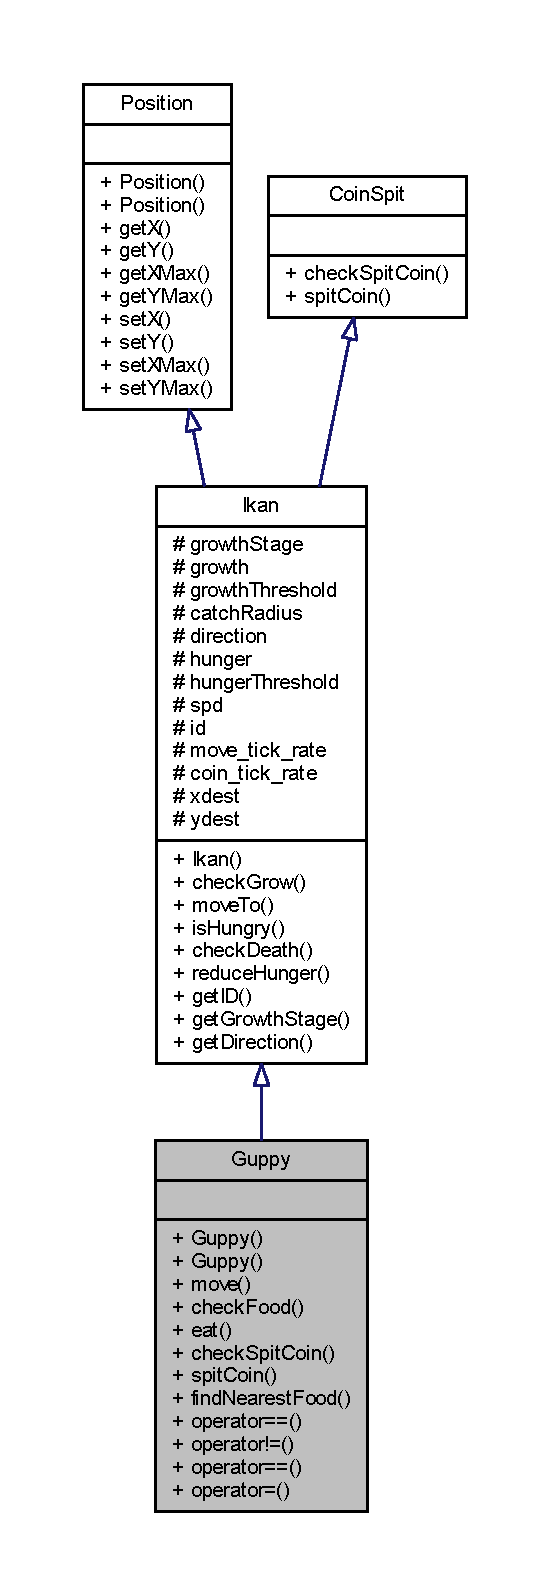
\includegraphics[width=204pt]{class_guppy__inherit__graph}
\end{center}
\end{figure}


Collaboration diagram for Guppy\+:\nopagebreak
\begin{figure}[H]
\begin{center}
\leavevmode
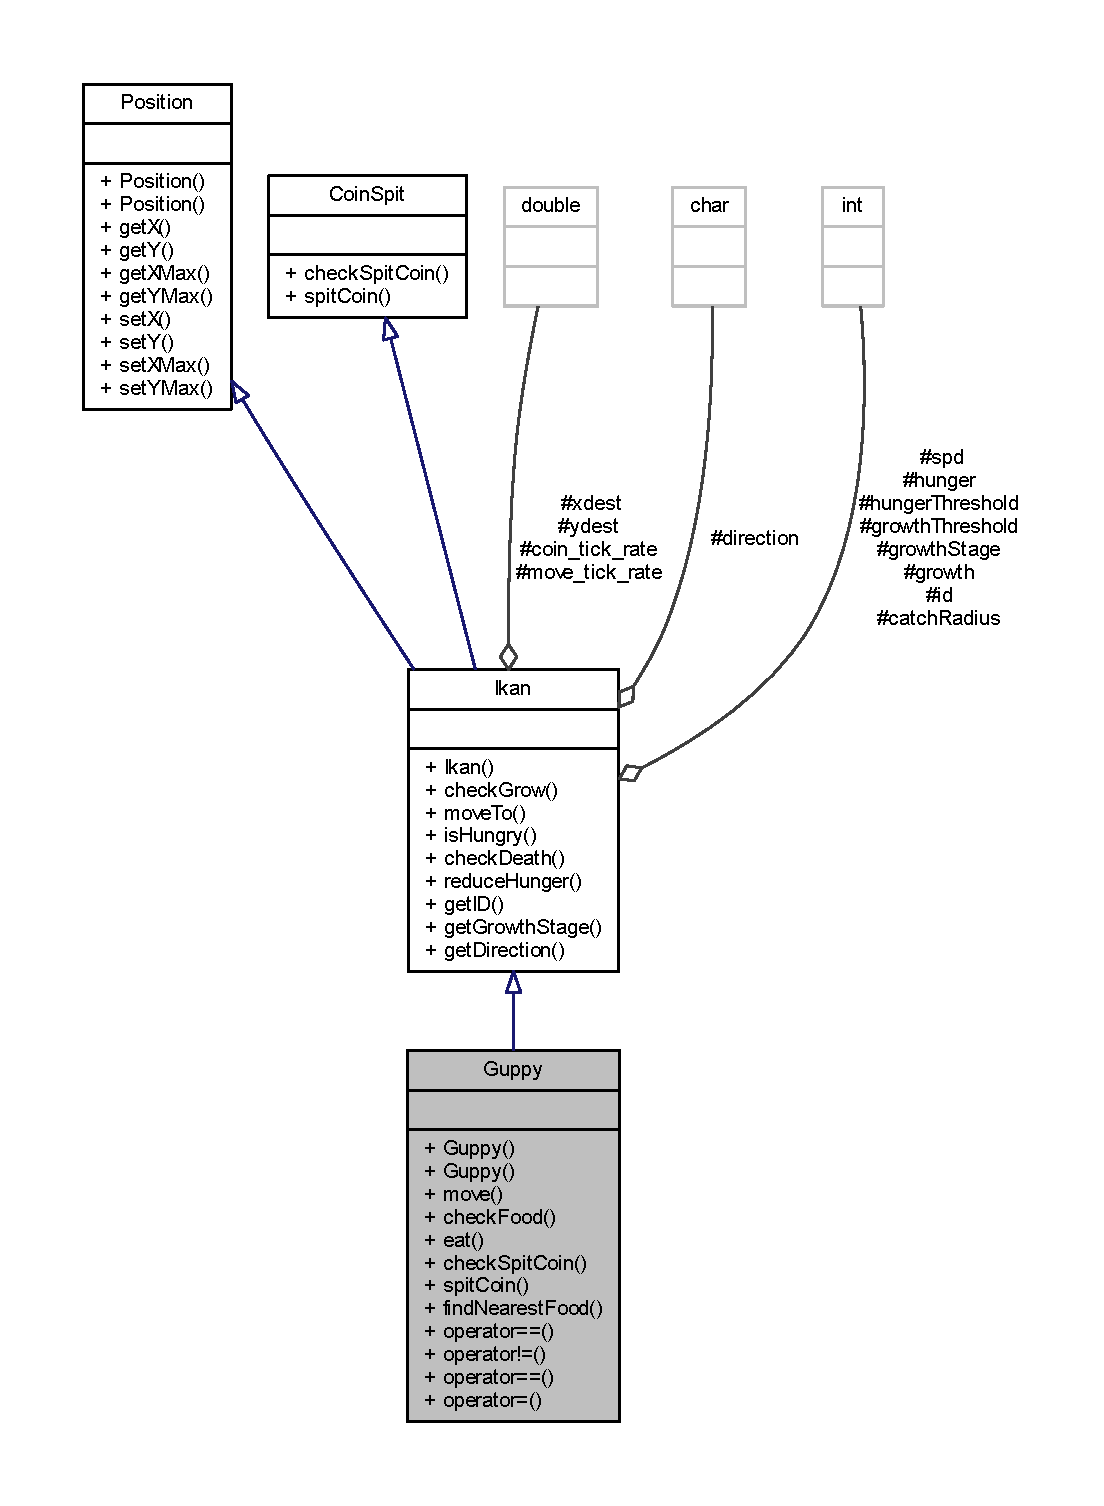
\includegraphics[width=204pt]{class_guppy__coll__graph}
\end{center}
\end{figure}
\subsection*{Public Member Functions}
\begin{DoxyCompactItemize}
\item 
\mbox{\hyperlink{class_guppy_aa78f8b5323b1015c968a8edab52773f5}{Guppy}} ()
\item 
\mbox{\hyperlink{class_guppy_a887d984014e34e1ea918b39c5698ee42}{Guppy}} (int x, int y, int xmax, int ymax)
\item 
void \mbox{\hyperlink{class_guppy_ac6ca65d23a87ab54f0b82f5c45082776}{move}} (\mbox{\hyperlink{class_list}{List}}$<$ \mbox{\hyperlink{class_makanan}{Makanan}} $>$ \&makanan, double sec\+\_\+since\+\_\+last)
\item 
bool \mbox{\hyperlink{class_guppy_a34ca887a2c2ff3b3fba494d0abd31bda}{check\+Food}} (\mbox{\hyperlink{class_list}{List}}$<$ \mbox{\hyperlink{class_makanan}{Makanan}} $>$ \&makanan)
\item 
void \mbox{\hyperlink{class_guppy_a03f670d2a9f6a6a28d3028d806fda979}{eat}} (\mbox{\hyperlink{class_list}{List}}$<$ \mbox{\hyperlink{class_makanan}{Makanan}} $>$ \&makanan)
\item 
bool \mbox{\hyperlink{class_guppy_abab3975de3a054b14aa3b8e664e30b5b}{check\+Spit\+Coin}} ()
\item 
void \mbox{\hyperlink{class_guppy_a39dfc2b44aed14f056bddcc08ff7c598}{spit\+Coin}} (\mbox{\hyperlink{class_list}{List}}$<$ \mbox{\hyperlink{class_coin}{Coin}} $>$ \&Lcoin, int value)
\item 
\mbox{\hyperlink{class_makanan}{Makanan}} $\ast$ \mbox{\hyperlink{class_guppy_accaa1f62989d00f7859f56848009089a}{find\+Nearest\+Food}} (\mbox{\hyperlink{class_list}{List}}$<$ \mbox{\hyperlink{class_makanan}{Makanan}} $>$ \&makanan)
\item 
bool \mbox{\hyperlink{class_guppy_a02efb73289d3b94264fba7d6c1d985b8}{operator==}} (const \mbox{\hyperlink{class_guppy}{Guppy}} \&G)
\item 
bool \mbox{\hyperlink{class_guppy_aa872357ac2df872e8b748066d6b79556}{operator!=}} (const \mbox{\hyperlink{class_guppy}{Guppy}} \&G)
\item 
bool \mbox{\hyperlink{class_guppy_a8b7c06fba5a291556cd4bf5255ac153e}{operator==}} (std\+::nullptr\+\_\+t n)
\item 
\mbox{\hyperlink{class_guppy}{Guppy}} \mbox{\hyperlink{class_guppy_aa30f6db726124f670123daadb53a581f}{operator=}} (const \mbox{\hyperlink{class_guppy}{Guppy}} \&G)
\end{DoxyCompactItemize}
\subsection*{Additional Inherited Members}


\subsection{Constructor \& Destructor Documentation}
\mbox{\Hypertarget{class_guppy_aa78f8b5323b1015c968a8edab52773f5}\label{class_guppy_aa78f8b5323b1015c968a8edab52773f5}} 
\index{Guppy@{Guppy}!Guppy@{Guppy}}
\index{Guppy@{Guppy}!Guppy@{Guppy}}
\subsubsection{\texorpdfstring{Guppy()}{Guppy()}\hspace{0.1cm}{\footnotesize\ttfamily [1/2]}}
{\footnotesize\ttfamily Guppy\+::\+Guppy (\begin{DoxyParamCaption}{ }\end{DoxyParamCaption})}

\mbox{\Hypertarget{class_guppy_a887d984014e34e1ea918b39c5698ee42}\label{class_guppy_a887d984014e34e1ea918b39c5698ee42}} 
\index{Guppy@{Guppy}!Guppy@{Guppy}}
\index{Guppy@{Guppy}!Guppy@{Guppy}}
\subsubsection{\texorpdfstring{Guppy()}{Guppy()}\hspace{0.1cm}{\footnotesize\ttfamily [2/2]}}
{\footnotesize\ttfamily Guppy\+::\+Guppy (\begin{DoxyParamCaption}\item[{int}]{x,  }\item[{int}]{y,  }\item[{int}]{xmax,  }\item[{int}]{ymax }\end{DoxyParamCaption})}



\subsection{Member Function Documentation}
\mbox{\Hypertarget{class_guppy_a34ca887a2c2ff3b3fba494d0abd31bda}\label{class_guppy_a34ca887a2c2ff3b3fba494d0abd31bda}} 
\index{Guppy@{Guppy}!check\+Food@{check\+Food}}
\index{check\+Food@{check\+Food}!Guppy@{Guppy}}
\subsubsection{\texorpdfstring{check\+Food()}{checkFood()}}
{\footnotesize\ttfamily bool Guppy\+::check\+Food (\begin{DoxyParamCaption}\item[{\mbox{\hyperlink{class_list}{List}}$<$ \mbox{\hyperlink{class_makanan}{Makanan}} $>$ \&}]{makanan }\end{DoxyParamCaption})}

\mbox{\Hypertarget{class_guppy_abab3975de3a054b14aa3b8e664e30b5b}\label{class_guppy_abab3975de3a054b14aa3b8e664e30b5b}} 
\index{Guppy@{Guppy}!check\+Spit\+Coin@{check\+Spit\+Coin}}
\index{check\+Spit\+Coin@{check\+Spit\+Coin}!Guppy@{Guppy}}
\subsubsection{\texorpdfstring{check\+Spit\+Coin()}{checkSpitCoin()}}
{\footnotesize\ttfamily bool Guppy\+::check\+Spit\+Coin (\begin{DoxyParamCaption}{ }\end{DoxyParamCaption})\hspace{0.3cm}{\ttfamily [virtual]}}



Implements \mbox{\hyperlink{class_coin_spit_a9471108f825dc67a35ac1a35444b84fd}{Coin\+Spit}}.

\mbox{\Hypertarget{class_guppy_a03f670d2a9f6a6a28d3028d806fda979}\label{class_guppy_a03f670d2a9f6a6a28d3028d806fda979}} 
\index{Guppy@{Guppy}!eat@{eat}}
\index{eat@{eat}!Guppy@{Guppy}}
\subsubsection{\texorpdfstring{eat()}{eat()}}
{\footnotesize\ttfamily void Guppy\+::eat (\begin{DoxyParamCaption}\item[{\mbox{\hyperlink{class_list}{List}}$<$ \mbox{\hyperlink{class_makanan}{Makanan}} $>$ \&}]{makanan }\end{DoxyParamCaption})}

\mbox{\Hypertarget{class_guppy_accaa1f62989d00f7859f56848009089a}\label{class_guppy_accaa1f62989d00f7859f56848009089a}} 
\index{Guppy@{Guppy}!find\+Nearest\+Food@{find\+Nearest\+Food}}
\index{find\+Nearest\+Food@{find\+Nearest\+Food}!Guppy@{Guppy}}
\subsubsection{\texorpdfstring{find\+Nearest\+Food()}{findNearestFood()}}
{\footnotesize\ttfamily \mbox{\hyperlink{class_makanan}{Makanan}} $\ast$ Guppy\+::find\+Nearest\+Food (\begin{DoxyParamCaption}\item[{\mbox{\hyperlink{class_list}{List}}$<$ \mbox{\hyperlink{class_makanan}{Makanan}} $>$ \&}]{makanan }\end{DoxyParamCaption})}

\mbox{\Hypertarget{class_guppy_ac6ca65d23a87ab54f0b82f5c45082776}\label{class_guppy_ac6ca65d23a87ab54f0b82f5c45082776}} 
\index{Guppy@{Guppy}!move@{move}}
\index{move@{move}!Guppy@{Guppy}}
\subsubsection{\texorpdfstring{move()}{move()}}
{\footnotesize\ttfamily void Guppy\+::move (\begin{DoxyParamCaption}\item[{\mbox{\hyperlink{class_list}{List}}$<$ \mbox{\hyperlink{class_makanan}{Makanan}} $>$ \&}]{makanan,  }\item[{double}]{sec\+\_\+since\+\_\+last }\end{DoxyParamCaption})}

\mbox{\Hypertarget{class_guppy_aa872357ac2df872e8b748066d6b79556}\label{class_guppy_aa872357ac2df872e8b748066d6b79556}} 
\index{Guppy@{Guppy}!operator"!=@{operator"!=}}
\index{operator"!=@{operator"!=}!Guppy@{Guppy}}
\subsubsection{\texorpdfstring{operator"!=()}{operator!=()}}
{\footnotesize\ttfamily bool Guppy\+::operator!= (\begin{DoxyParamCaption}\item[{const \mbox{\hyperlink{class_guppy}{Guppy}} \&}]{G }\end{DoxyParamCaption})}

\mbox{\Hypertarget{class_guppy_aa30f6db726124f670123daadb53a581f}\label{class_guppy_aa30f6db726124f670123daadb53a581f}} 
\index{Guppy@{Guppy}!operator=@{operator=}}
\index{operator=@{operator=}!Guppy@{Guppy}}
\subsubsection{\texorpdfstring{operator=()}{operator=()}}
{\footnotesize\ttfamily \mbox{\hyperlink{class_guppy}{Guppy}} Guppy\+::operator= (\begin{DoxyParamCaption}\item[{const \mbox{\hyperlink{class_guppy}{Guppy}} \&}]{G }\end{DoxyParamCaption})}

\mbox{\Hypertarget{class_guppy_a02efb73289d3b94264fba7d6c1d985b8}\label{class_guppy_a02efb73289d3b94264fba7d6c1d985b8}} 
\index{Guppy@{Guppy}!operator==@{operator==}}
\index{operator==@{operator==}!Guppy@{Guppy}}
\subsubsection{\texorpdfstring{operator==()}{operator==()}\hspace{0.1cm}{\footnotesize\ttfamily [1/2]}}
{\footnotesize\ttfamily bool Guppy\+::operator== (\begin{DoxyParamCaption}\item[{const \mbox{\hyperlink{class_guppy}{Guppy}} \&}]{G }\end{DoxyParamCaption})}

\mbox{\Hypertarget{class_guppy_a8b7c06fba5a291556cd4bf5255ac153e}\label{class_guppy_a8b7c06fba5a291556cd4bf5255ac153e}} 
\index{Guppy@{Guppy}!operator==@{operator==}}
\index{operator==@{operator==}!Guppy@{Guppy}}
\subsubsection{\texorpdfstring{operator==()}{operator==()}\hspace{0.1cm}{\footnotesize\ttfamily [2/2]}}
{\footnotesize\ttfamily bool Guppy\+::operator== (\begin{DoxyParamCaption}\item[{std\+::nullptr\+\_\+t}]{n }\end{DoxyParamCaption})}

\mbox{\Hypertarget{class_guppy_a39dfc2b44aed14f056bddcc08ff7c598}\label{class_guppy_a39dfc2b44aed14f056bddcc08ff7c598}} 
\index{Guppy@{Guppy}!spit\+Coin@{spit\+Coin}}
\index{spit\+Coin@{spit\+Coin}!Guppy@{Guppy}}
\subsubsection{\texorpdfstring{spit\+Coin()}{spitCoin()}}
{\footnotesize\ttfamily void Guppy\+::spit\+Coin (\begin{DoxyParamCaption}\item[{\mbox{\hyperlink{class_list}{List}}$<$ \mbox{\hyperlink{class_coin}{Coin}} $>$ \&}]{Lcoin,  }\item[{int}]{value }\end{DoxyParamCaption})\hspace{0.3cm}{\ttfamily [virtual]}}



Implements \mbox{\hyperlink{class_coin_spit_a336f45a90c4b0b57017b45a5c68f12a7}{Coin\+Spit}}.



The documentation for this class was generated from the following files\+:\begin{DoxyCompactItemize}
\item 
headers/\mbox{\hyperlink{_guppy_8hpp}{Guppy.\+hpp}}\item 
src/\mbox{\hyperlink{_guppy_8cpp}{Guppy.\+cpp}}\end{DoxyCompactItemize}

\hypertarget{class_ikan}{}\section{Ikan Class Reference}
\label{class_ikan}\index{Ikan@{Ikan}}


{\ttfamily \#include $<$Ikan.\+hpp$>$}



Inheritance diagram for Ikan\+:
\nopagebreak
\begin{figure}[H]
\begin{center}
\leavevmode
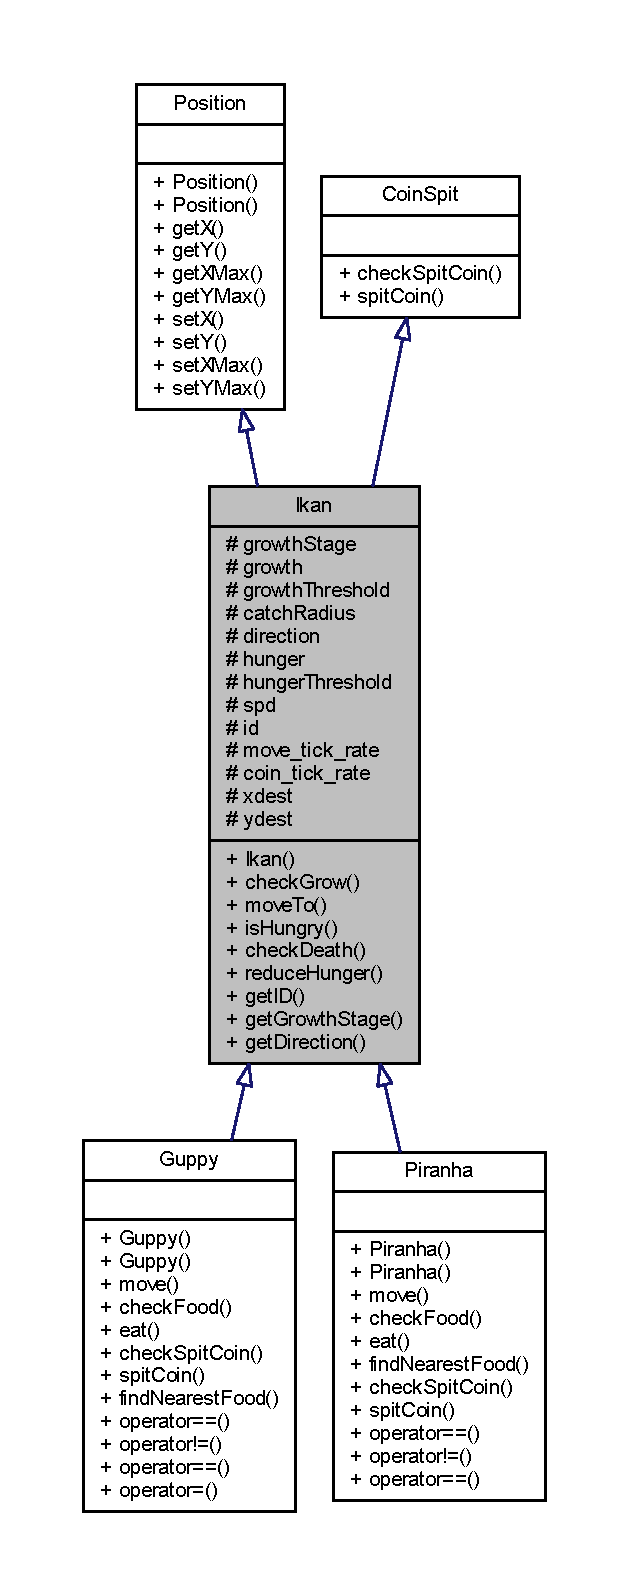
\includegraphics[height=550pt]{class_ikan__inherit__graph}
\end{center}
\end{figure}


Collaboration diagram for Ikan\+:
\nopagebreak
\begin{figure}[H]
\begin{center}
\leavevmode
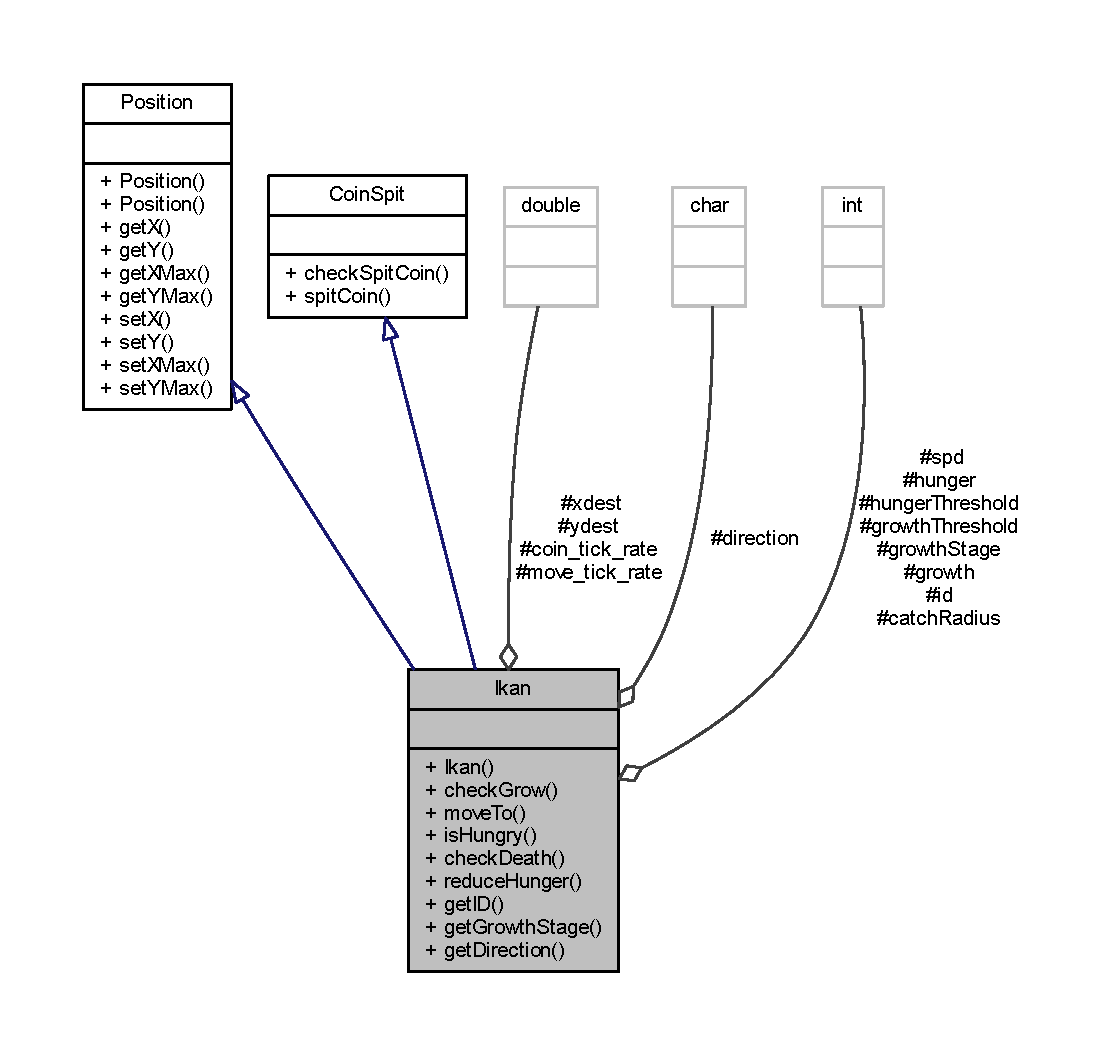
\includegraphics[width=350pt]{class_ikan__coll__graph}
\end{center}
\end{figure}
\subsection*{Public Member Functions}
\begin{DoxyCompactItemize}
\item 
\mbox{\hyperlink{class_ikan_a0770a992c26f08ba3d9bad79fec71d55}{Ikan}} (int x, int y, int xmax, int ymax, int g\+Threshold, int c\+Radius, int h\+Threshold, int \mbox{\hyperlink{class_ikan_aac75c79c60a94f5607bdc2730203fd6f}{spd}}, int \mbox{\hyperlink{class_ikan_a9af33ebcd489980e17cbd4b876692e85}{id}})
\item 
void \mbox{\hyperlink{class_ikan_a68425d0df0528611318bdbef89aaf039}{check\+Grow}} ()
\item 
void \mbox{\hyperlink{class_ikan_af1b9d17721061771c7ea855b9c6e301d}{move\+To}} (int x, int y, double sec\+\_\+since\+\_\+last)
\item 
bool \mbox{\hyperlink{class_ikan_a893df179377af8174785228240eead8d}{is\+Hungry}} ()
\item 
bool \mbox{\hyperlink{class_ikan_a9a607ca1962b8f6029562e5571eaeb5c}{check\+Death}} ()
\item 
void \mbox{\hyperlink{class_ikan_aadb3eab63a3277d12d0cd4af5a9c96aa}{reduce\+Hunger}} (double sec)
\item 
int \mbox{\hyperlink{class_ikan_aa047dd2004a534353200f274e1541127}{get\+ID}} ()
\item 
int \mbox{\hyperlink{class_ikan_aa224e500b9f7c1f1e39b6045041a0d2f}{get\+Growth\+Stage}} ()
\item 
char \mbox{\hyperlink{class_ikan_af92d7548a85251152d24c6906c504298}{get\+Direction}} ()
\end{DoxyCompactItemize}
\subsection*{Protected Attributes}
\begin{DoxyCompactItemize}
\item 
int \mbox{\hyperlink{class_ikan_aad3d87c6a66aa4cf3ec9e47b37bc90e3}{growth\+Stage}}
\item 
int \mbox{\hyperlink{class_ikan_a8c8f1efec43b4ae815d88b6472bc81bb}{growth}}
\item 
const int \mbox{\hyperlink{class_ikan_a7eaddebc6127b66ddfad007f49b4ae83}{growth\+Threshold}}
\item 
const int \mbox{\hyperlink{class_ikan_a7d6507a938bda54ba96d224e27a12b71}{catch\+Radius}}
\item 
char \mbox{\hyperlink{class_ikan_ac0fdc43f8926aaa17b0deb0ebfd4cc5b}{direction}}
\item 
int \mbox{\hyperlink{class_ikan_a038bd5c59db6efca6dc0e722a182ff09}{hunger}}
\item 
const int \mbox{\hyperlink{class_ikan_ac9671ac93e29bd9de93f401ecc903ac9}{hunger\+Threshold}}
\item 
int \mbox{\hyperlink{class_ikan_aac75c79c60a94f5607bdc2730203fd6f}{spd}}
\item 
int \mbox{\hyperlink{class_ikan_a9af33ebcd489980e17cbd4b876692e85}{id}}
\item 
double \mbox{\hyperlink{class_ikan_a51d3fe38edbf39ca78308b5d20630a77}{move\+\_\+tick\+\_\+rate}}
\item 
double \mbox{\hyperlink{class_ikan_af6c55901dcc5cfbdcc8b30798949118e}{coin\+\_\+tick\+\_\+rate}}
\item 
double \mbox{\hyperlink{class_ikan_a8c240f6477e1010fa7d70e505bf66ae3}{xdest}}
\item 
double \mbox{\hyperlink{class_ikan_ac338da0dc5dd61ec09b279200f94d328}{ydest}}
\end{DoxyCompactItemize}


\subsection{Constructor \& Destructor Documentation}
\mbox{\Hypertarget{class_ikan_a0770a992c26f08ba3d9bad79fec71d55}\label{class_ikan_a0770a992c26f08ba3d9bad79fec71d55}} 
\index{Ikan@{Ikan}!Ikan@{Ikan}}
\index{Ikan@{Ikan}!Ikan@{Ikan}}
\subsubsection{\texorpdfstring{Ikan()}{Ikan()}}
{\footnotesize\ttfamily Ikan\+::\+Ikan (\begin{DoxyParamCaption}\item[{int}]{x,  }\item[{int}]{y,  }\item[{int}]{xmax,  }\item[{int}]{ymax,  }\item[{int}]{g\+Threshold,  }\item[{int}]{c\+Radius,  }\item[{int}]{h\+Threshold,  }\item[{int}]{spd,  }\item[{int}]{id }\end{DoxyParamCaption})}



\subsection{Member Function Documentation}
\mbox{\Hypertarget{class_ikan_a9a607ca1962b8f6029562e5571eaeb5c}\label{class_ikan_a9a607ca1962b8f6029562e5571eaeb5c}} 
\index{Ikan@{Ikan}!check\+Death@{check\+Death}}
\index{check\+Death@{check\+Death}!Ikan@{Ikan}}
\subsubsection{\texorpdfstring{check\+Death()}{checkDeath()}}
{\footnotesize\ttfamily bool Ikan\+::check\+Death (\begin{DoxyParamCaption}{ }\end{DoxyParamCaption})}

\mbox{\Hypertarget{class_ikan_a68425d0df0528611318bdbef89aaf039}\label{class_ikan_a68425d0df0528611318bdbef89aaf039}} 
\index{Ikan@{Ikan}!check\+Grow@{check\+Grow}}
\index{check\+Grow@{check\+Grow}!Ikan@{Ikan}}
\subsubsection{\texorpdfstring{check\+Grow()}{checkGrow()}}
{\footnotesize\ttfamily void Ikan\+::check\+Grow (\begin{DoxyParamCaption}{ }\end{DoxyParamCaption})}

\mbox{\Hypertarget{class_ikan_af92d7548a85251152d24c6906c504298}\label{class_ikan_af92d7548a85251152d24c6906c504298}} 
\index{Ikan@{Ikan}!get\+Direction@{get\+Direction}}
\index{get\+Direction@{get\+Direction}!Ikan@{Ikan}}
\subsubsection{\texorpdfstring{get\+Direction()}{getDirection()}}
{\footnotesize\ttfamily char Ikan\+::get\+Direction (\begin{DoxyParamCaption}{ }\end{DoxyParamCaption})}

\mbox{\Hypertarget{class_ikan_aa224e500b9f7c1f1e39b6045041a0d2f}\label{class_ikan_aa224e500b9f7c1f1e39b6045041a0d2f}} 
\index{Ikan@{Ikan}!get\+Growth\+Stage@{get\+Growth\+Stage}}
\index{get\+Growth\+Stage@{get\+Growth\+Stage}!Ikan@{Ikan}}
\subsubsection{\texorpdfstring{get\+Growth\+Stage()}{getGrowthStage()}}
{\footnotesize\ttfamily int Ikan\+::get\+Growth\+Stage (\begin{DoxyParamCaption}{ }\end{DoxyParamCaption})}

\mbox{\Hypertarget{class_ikan_aa047dd2004a534353200f274e1541127}\label{class_ikan_aa047dd2004a534353200f274e1541127}} 
\index{Ikan@{Ikan}!get\+ID@{get\+ID}}
\index{get\+ID@{get\+ID}!Ikan@{Ikan}}
\subsubsection{\texorpdfstring{get\+I\+D()}{getID()}}
{\footnotesize\ttfamily int Ikan\+::get\+ID (\begin{DoxyParamCaption}{ }\end{DoxyParamCaption})}

\mbox{\Hypertarget{class_ikan_a893df179377af8174785228240eead8d}\label{class_ikan_a893df179377af8174785228240eead8d}} 
\index{Ikan@{Ikan}!is\+Hungry@{is\+Hungry}}
\index{is\+Hungry@{is\+Hungry}!Ikan@{Ikan}}
\subsubsection{\texorpdfstring{is\+Hungry()}{isHungry()}}
{\footnotesize\ttfamily bool Ikan\+::is\+Hungry (\begin{DoxyParamCaption}{ }\end{DoxyParamCaption})}

\mbox{\Hypertarget{class_ikan_af1b9d17721061771c7ea855b9c6e301d}\label{class_ikan_af1b9d17721061771c7ea855b9c6e301d}} 
\index{Ikan@{Ikan}!move\+To@{move\+To}}
\index{move\+To@{move\+To}!Ikan@{Ikan}}
\subsubsection{\texorpdfstring{move\+To()}{moveTo()}}
{\footnotesize\ttfamily void Ikan\+::move\+To (\begin{DoxyParamCaption}\item[{int}]{x,  }\item[{int}]{y,  }\item[{double}]{sec\+\_\+since\+\_\+last }\end{DoxyParamCaption})}

\mbox{\Hypertarget{class_ikan_aadb3eab63a3277d12d0cd4af5a9c96aa}\label{class_ikan_aadb3eab63a3277d12d0cd4af5a9c96aa}} 
\index{Ikan@{Ikan}!reduce\+Hunger@{reduce\+Hunger}}
\index{reduce\+Hunger@{reduce\+Hunger}!Ikan@{Ikan}}
\subsubsection{\texorpdfstring{reduce\+Hunger()}{reduceHunger()}}
{\footnotesize\ttfamily void Ikan\+::reduce\+Hunger (\begin{DoxyParamCaption}\item[{double}]{sec }\end{DoxyParamCaption})}



\subsection{Member Data Documentation}
\mbox{\Hypertarget{class_ikan_a7d6507a938bda54ba96d224e27a12b71}\label{class_ikan_a7d6507a938bda54ba96d224e27a12b71}} 
\index{Ikan@{Ikan}!catch\+Radius@{catch\+Radius}}
\index{catch\+Radius@{catch\+Radius}!Ikan@{Ikan}}
\subsubsection{\texorpdfstring{catch\+Radius}{catchRadius}}
{\footnotesize\ttfamily const int Ikan\+::catch\+Radius\hspace{0.3cm}{\ttfamily [protected]}}

\mbox{\Hypertarget{class_ikan_af6c55901dcc5cfbdcc8b30798949118e}\label{class_ikan_af6c55901dcc5cfbdcc8b30798949118e}} 
\index{Ikan@{Ikan}!coin\+\_\+tick\+\_\+rate@{coin\+\_\+tick\+\_\+rate}}
\index{coin\+\_\+tick\+\_\+rate@{coin\+\_\+tick\+\_\+rate}!Ikan@{Ikan}}
\subsubsection{\texorpdfstring{coin\+\_\+tick\+\_\+rate}{coin\_tick\_rate}}
{\footnotesize\ttfamily double Ikan\+::coin\+\_\+tick\+\_\+rate\hspace{0.3cm}{\ttfamily [protected]}}

\mbox{\Hypertarget{class_ikan_ac0fdc43f8926aaa17b0deb0ebfd4cc5b}\label{class_ikan_ac0fdc43f8926aaa17b0deb0ebfd4cc5b}} 
\index{Ikan@{Ikan}!direction@{direction}}
\index{direction@{direction}!Ikan@{Ikan}}
\subsubsection{\texorpdfstring{direction}{direction}}
{\footnotesize\ttfamily char Ikan\+::direction\hspace{0.3cm}{\ttfamily [protected]}}

\mbox{\Hypertarget{class_ikan_a8c8f1efec43b4ae815d88b6472bc81bb}\label{class_ikan_a8c8f1efec43b4ae815d88b6472bc81bb}} 
\index{Ikan@{Ikan}!growth@{growth}}
\index{growth@{growth}!Ikan@{Ikan}}
\subsubsection{\texorpdfstring{growth}{growth}}
{\footnotesize\ttfamily int Ikan\+::growth\hspace{0.3cm}{\ttfamily [protected]}}

\mbox{\Hypertarget{class_ikan_aad3d87c6a66aa4cf3ec9e47b37bc90e3}\label{class_ikan_aad3d87c6a66aa4cf3ec9e47b37bc90e3}} 
\index{Ikan@{Ikan}!growth\+Stage@{growth\+Stage}}
\index{growth\+Stage@{growth\+Stage}!Ikan@{Ikan}}
\subsubsection{\texorpdfstring{growth\+Stage}{growthStage}}
{\footnotesize\ttfamily int Ikan\+::growth\+Stage\hspace{0.3cm}{\ttfamily [protected]}}

\mbox{\Hypertarget{class_ikan_a7eaddebc6127b66ddfad007f49b4ae83}\label{class_ikan_a7eaddebc6127b66ddfad007f49b4ae83}} 
\index{Ikan@{Ikan}!growth\+Threshold@{growth\+Threshold}}
\index{growth\+Threshold@{growth\+Threshold}!Ikan@{Ikan}}
\subsubsection{\texorpdfstring{growth\+Threshold}{growthThreshold}}
{\footnotesize\ttfamily const int Ikan\+::growth\+Threshold\hspace{0.3cm}{\ttfamily [protected]}}

\mbox{\Hypertarget{class_ikan_a038bd5c59db6efca6dc0e722a182ff09}\label{class_ikan_a038bd5c59db6efca6dc0e722a182ff09}} 
\index{Ikan@{Ikan}!hunger@{hunger}}
\index{hunger@{hunger}!Ikan@{Ikan}}
\subsubsection{\texorpdfstring{hunger}{hunger}}
{\footnotesize\ttfamily int Ikan\+::hunger\hspace{0.3cm}{\ttfamily [protected]}}

\mbox{\Hypertarget{class_ikan_ac9671ac93e29bd9de93f401ecc903ac9}\label{class_ikan_ac9671ac93e29bd9de93f401ecc903ac9}} 
\index{Ikan@{Ikan}!hunger\+Threshold@{hunger\+Threshold}}
\index{hunger\+Threshold@{hunger\+Threshold}!Ikan@{Ikan}}
\subsubsection{\texorpdfstring{hunger\+Threshold}{hungerThreshold}}
{\footnotesize\ttfamily const int Ikan\+::hunger\+Threshold\hspace{0.3cm}{\ttfamily [protected]}}

\mbox{\Hypertarget{class_ikan_a9af33ebcd489980e17cbd4b876692e85}\label{class_ikan_a9af33ebcd489980e17cbd4b876692e85}} 
\index{Ikan@{Ikan}!id@{id}}
\index{id@{id}!Ikan@{Ikan}}
\subsubsection{\texorpdfstring{id}{id}}
{\footnotesize\ttfamily int Ikan\+::id\hspace{0.3cm}{\ttfamily [protected]}}

\mbox{\Hypertarget{class_ikan_a51d3fe38edbf39ca78308b5d20630a77}\label{class_ikan_a51d3fe38edbf39ca78308b5d20630a77}} 
\index{Ikan@{Ikan}!move\+\_\+tick\+\_\+rate@{move\+\_\+tick\+\_\+rate}}
\index{move\+\_\+tick\+\_\+rate@{move\+\_\+tick\+\_\+rate}!Ikan@{Ikan}}
\subsubsection{\texorpdfstring{move\+\_\+tick\+\_\+rate}{move\_tick\_rate}}
{\footnotesize\ttfamily double Ikan\+::move\+\_\+tick\+\_\+rate\hspace{0.3cm}{\ttfamily [protected]}}

\mbox{\Hypertarget{class_ikan_aac75c79c60a94f5607bdc2730203fd6f}\label{class_ikan_aac75c79c60a94f5607bdc2730203fd6f}} 
\index{Ikan@{Ikan}!spd@{spd}}
\index{spd@{spd}!Ikan@{Ikan}}
\subsubsection{\texorpdfstring{spd}{spd}}
{\footnotesize\ttfamily int Ikan\+::spd\hspace{0.3cm}{\ttfamily [protected]}}

\mbox{\Hypertarget{class_ikan_a8c240f6477e1010fa7d70e505bf66ae3}\label{class_ikan_a8c240f6477e1010fa7d70e505bf66ae3}} 
\index{Ikan@{Ikan}!xdest@{xdest}}
\index{xdest@{xdest}!Ikan@{Ikan}}
\subsubsection{\texorpdfstring{xdest}{xdest}}
{\footnotesize\ttfamily double Ikan\+::xdest\hspace{0.3cm}{\ttfamily [protected]}}

\mbox{\Hypertarget{class_ikan_ac338da0dc5dd61ec09b279200f94d328}\label{class_ikan_ac338da0dc5dd61ec09b279200f94d328}} 
\index{Ikan@{Ikan}!ydest@{ydest}}
\index{ydest@{ydest}!Ikan@{Ikan}}
\subsubsection{\texorpdfstring{ydest}{ydest}}
{\footnotesize\ttfamily double Ikan\+::ydest\hspace{0.3cm}{\ttfamily [protected]}}



The documentation for this class was generated from the following files\+:\begin{DoxyCompactItemize}
\item 
C\+:/\+Users/user/\+Desktop/technical stuff/cpp/\+Tubes O\+O\+P/\+Main Folder/headers/\mbox{\hyperlink{_ikan_8hpp}{Ikan.\+hpp}}\item 
C\+:/\+Users/user/\+Desktop/technical stuff/cpp/\+Tubes O\+O\+P/\+Main Folder/src/\mbox{\hyperlink{_ikan_8cpp}{Ikan.\+cpp}}\end{DoxyCompactItemize}

\hypertarget{class_list}{}\section{List$<$ T $>$ Class Template Reference}
\label{class_list}\index{List$<$ T $>$@{List$<$ T $>$}}


{\ttfamily \#include $<$List.\+hpp$>$}



Inheritance diagram for List$<$ T $>$\+:
\nopagebreak
\begin{figure}[H]
\begin{center}
\leavevmode
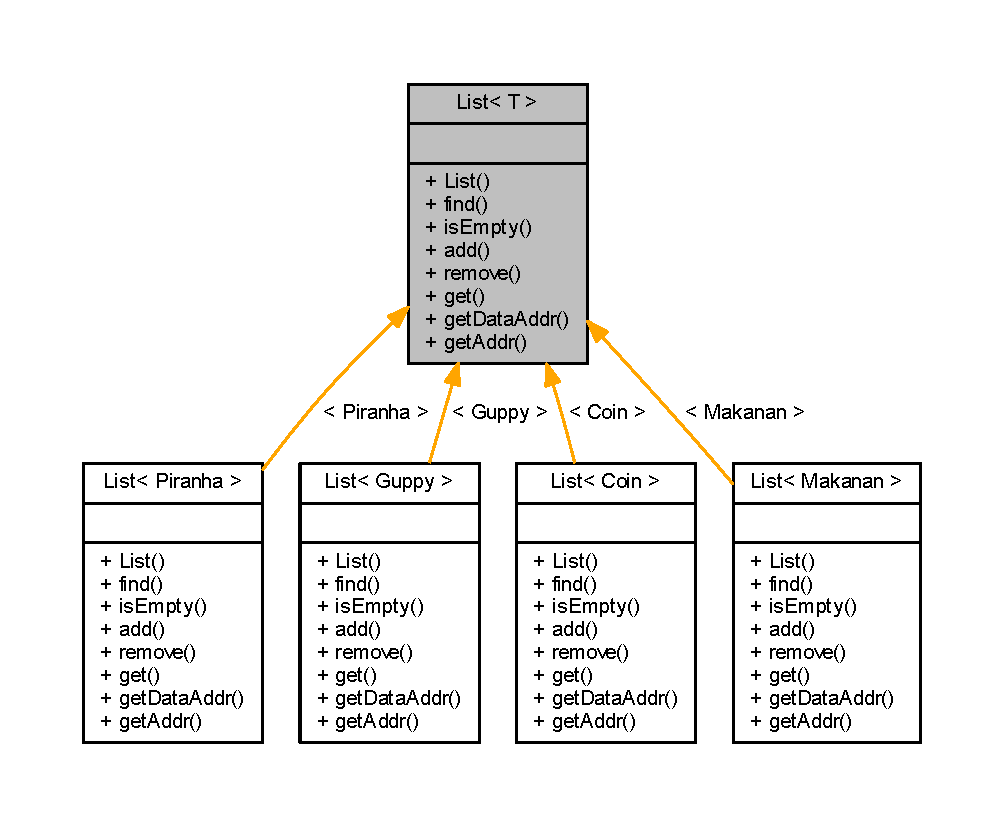
\includegraphics[width=350pt]{class_list__inherit__graph}
\end{center}
\end{figure}


Collaboration diagram for List$<$ T $>$\+:
\nopagebreak
\begin{figure}[H]
\begin{center}
\leavevmode
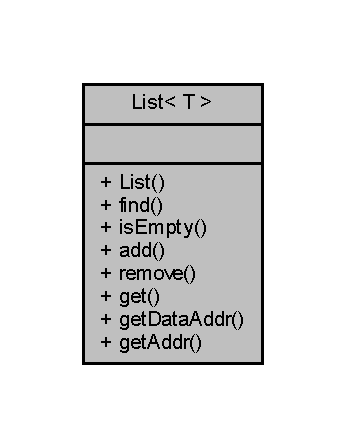
\includegraphics[width=166pt]{class_list__coll__graph}
\end{center}
\end{figure}
\subsection*{Public Member Functions}
\begin{DoxyCompactItemize}
\item 
\mbox{\hyperlink{class_list_a5c5e27671b21b3815d4e25b953c69454}{List}} ()
\item 
int \mbox{\hyperlink{class_list_afcc0ad2940d9efbd8b487bc40e3f0067}{find}} (T elmt)
\item 
bool \mbox{\hyperlink{class_list_a73f8b1d313382daffeeeed552f42da2f}{is\+Empty}} ()
\item 
void \mbox{\hyperlink{class_list_aea51297cc29bc89acf013d43636a6a19}{add}} (T $\ast$elmt)
\item 
void \mbox{\hyperlink{class_list_a7fac84accc112425caecf55c6b92911d}{remove}} (T elmt)
\item 
T \mbox{\hyperlink{class_list_a8674ced74b669f6c49292a4545c5b1e3}{get}} (int index)
\item 
T $\ast$ \mbox{\hyperlink{class_list_a09652510ae90b0f23ecfbc64fe81edc9}{get\+Data\+Addr}} (int index)
\item 
\mbox{\hyperlink{class_list}{List}}$<$ T $>$ $\ast$ \mbox{\hyperlink{class_list_ad34f9546e1bee20ecf23a985e34c3fb8}{get\+Addr}} (int index)
\end{DoxyCompactItemize}


\subsection{Constructor \& Destructor Documentation}
\mbox{\Hypertarget{class_list_a5c5e27671b21b3815d4e25b953c69454}\label{class_list_a5c5e27671b21b3815d4e25b953c69454}} 
\index{List@{List}!List@{List}}
\index{List@{List}!List@{List}}
\subsubsection{\texorpdfstring{List()}{List()}}
{\footnotesize\ttfamily template$<$class T $>$ \\
\mbox{\hyperlink{class_list}{List}}$<$ T $>$\+::\mbox{\hyperlink{class_list}{List}} (\begin{DoxyParamCaption}{ }\end{DoxyParamCaption})}



\subsection{Member Function Documentation}
\mbox{\Hypertarget{class_list_aea51297cc29bc89acf013d43636a6a19}\label{class_list_aea51297cc29bc89acf013d43636a6a19}} 
\index{List@{List}!add@{add}}
\index{add@{add}!List@{List}}
\subsubsection{\texorpdfstring{add()}{add()}}
{\footnotesize\ttfamily template$<$class T$>$ \\
void \mbox{\hyperlink{class_list}{List}}$<$ T $>$\+::add (\begin{DoxyParamCaption}\item[{T $\ast$}]{elmt }\end{DoxyParamCaption})}

\mbox{\Hypertarget{class_list_afcc0ad2940d9efbd8b487bc40e3f0067}\label{class_list_afcc0ad2940d9efbd8b487bc40e3f0067}} 
\index{List@{List}!find@{find}}
\index{find@{find}!List@{List}}
\subsubsection{\texorpdfstring{find()}{find()}}
{\footnotesize\ttfamily template$<$class T$>$ \\
int \mbox{\hyperlink{class_list}{List}}$<$ T $>$\+::find (\begin{DoxyParamCaption}\item[{T}]{elmt }\end{DoxyParamCaption})}

\mbox{\Hypertarget{class_list_a8674ced74b669f6c49292a4545c5b1e3}\label{class_list_a8674ced74b669f6c49292a4545c5b1e3}} 
\index{List@{List}!get@{get}}
\index{get@{get}!List@{List}}
\subsubsection{\texorpdfstring{get()}{get()}}
{\footnotesize\ttfamily template$<$class T $>$ \\
T \mbox{\hyperlink{class_list}{List}}$<$ T $>$\+::get (\begin{DoxyParamCaption}\item[{int}]{index }\end{DoxyParamCaption})}

\mbox{\Hypertarget{class_list_ad34f9546e1bee20ecf23a985e34c3fb8}\label{class_list_ad34f9546e1bee20ecf23a985e34c3fb8}} 
\index{List@{List}!get\+Addr@{get\+Addr}}
\index{get\+Addr@{get\+Addr}!List@{List}}
\subsubsection{\texorpdfstring{get\+Addr()}{getAddr()}}
{\footnotesize\ttfamily template$<$class T $>$ \\
\mbox{\hyperlink{class_list}{List}}$<$ T $>$ $\ast$ \mbox{\hyperlink{class_list}{List}}$<$ T $>$\+::get\+Addr (\begin{DoxyParamCaption}\item[{int}]{index }\end{DoxyParamCaption})}

\mbox{\Hypertarget{class_list_a09652510ae90b0f23ecfbc64fe81edc9}\label{class_list_a09652510ae90b0f23ecfbc64fe81edc9}} 
\index{List@{List}!get\+Data\+Addr@{get\+Data\+Addr}}
\index{get\+Data\+Addr@{get\+Data\+Addr}!List@{List}}
\subsubsection{\texorpdfstring{get\+Data\+Addr()}{getDataAddr()}}
{\footnotesize\ttfamily template$<$class T $>$ \\
T $\ast$ \mbox{\hyperlink{class_list}{List}}$<$ T $>$\+::get\+Data\+Addr (\begin{DoxyParamCaption}\item[{int}]{index }\end{DoxyParamCaption})}

\mbox{\Hypertarget{class_list_a73f8b1d313382daffeeeed552f42da2f}\label{class_list_a73f8b1d313382daffeeeed552f42da2f}} 
\index{List@{List}!is\+Empty@{is\+Empty}}
\index{is\+Empty@{is\+Empty}!List@{List}}
\subsubsection{\texorpdfstring{is\+Empty()}{isEmpty()}}
{\footnotesize\ttfamily template$<$class T $>$ \\
bool \mbox{\hyperlink{class_list}{List}}$<$ T $>$\+::is\+Empty (\begin{DoxyParamCaption}{ }\end{DoxyParamCaption})}

\mbox{\Hypertarget{class_list_a7fac84accc112425caecf55c6b92911d}\label{class_list_a7fac84accc112425caecf55c6b92911d}} 
\index{List@{List}!remove@{remove}}
\index{remove@{remove}!List@{List}}
\subsubsection{\texorpdfstring{remove()}{remove()}}
{\footnotesize\ttfamily template$<$class T$>$ \\
void \mbox{\hyperlink{class_list}{List}}$<$ T $>$\+::remove (\begin{DoxyParamCaption}\item[{T}]{elmt }\end{DoxyParamCaption})}



The documentation for this class was generated from the following file\+:\begin{DoxyCompactItemize}
\item 
C\+:/\+Users/user/\+Desktop/technical stuff/cpp/\+Tubes O\+O\+P/\+Main Folder/headers/\mbox{\hyperlink{_list_8hpp}{List.\+hpp}}\end{DoxyCompactItemize}

\hypertarget{class_makanan}{}\section{Makanan Class Reference}
\label{class_makanan}\index{Makanan@{Makanan}}


{\ttfamily \#include $<$Makanan.\+hpp$>$}



Inheritance diagram for Makanan\+:
\nopagebreak
\begin{figure}[H]
\begin{center}
\leavevmode
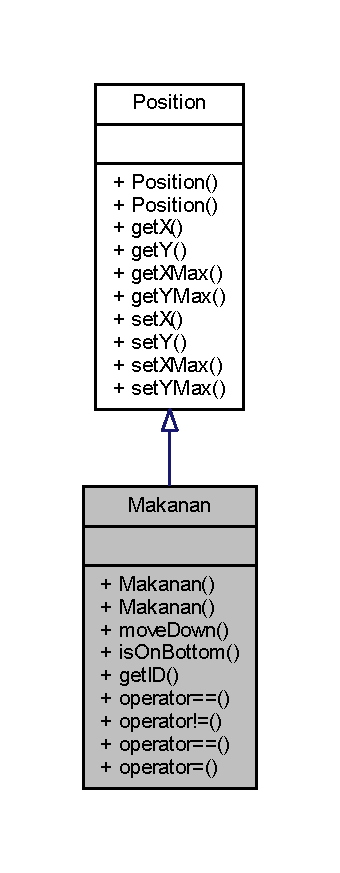
\includegraphics[width=163pt]{class_makanan__inherit__graph}
\end{center}
\end{figure}


Collaboration diagram for Makanan\+:
\nopagebreak
\begin{figure}[H]
\begin{center}
\leavevmode
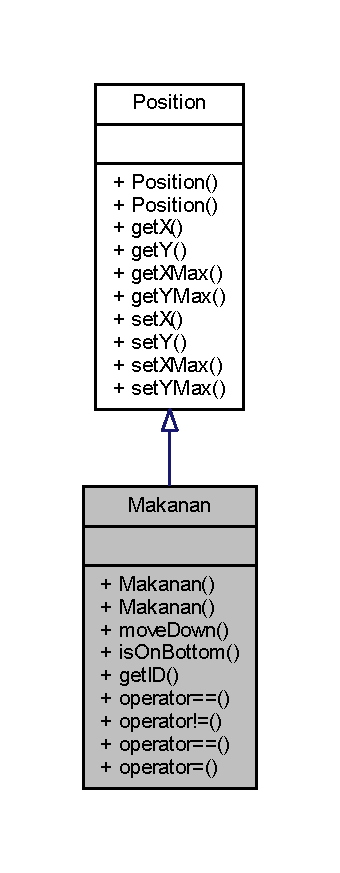
\includegraphics[width=163pt]{class_makanan__coll__graph}
\end{center}
\end{figure}
\subsection*{Public Member Functions}
\begin{DoxyCompactItemize}
\item 
\mbox{\hyperlink{class_makanan_a3123c9b9ca1a63c8334f617934faf634}{Makanan}} ()
\item 
\mbox{\hyperlink{class_makanan_a547f3e22ca69ff229ec25e3117dd96ed}{Makanan}} (int x, int y, int xmax, int ymax)
\item 
void \mbox{\hyperlink{class_makanan_abc0157c0c2133133104de97e1b1a07f0}{move\+Down}} (double sec\+\_\+since\+\_\+last)
\item 
bool \mbox{\hyperlink{class_makanan_a2d5537ee58ca99aed562aebdbb66de48}{is\+On\+Bottom}} ()
\item 
int \mbox{\hyperlink{class_makanan_a0af9a28dae90b5509cfd60e6f3046655}{get\+ID}} ()
\item 
bool \mbox{\hyperlink{class_makanan_aeee966e624eda92eb398f8236a6b914d}{operator==}} (const \mbox{\hyperlink{class_makanan}{Makanan}} \&M)
\item 
bool \mbox{\hyperlink{class_makanan_a832120fa6c5e08529fb3237d257b0d4d}{operator!=}} (const \mbox{\hyperlink{class_makanan}{Makanan}} \&M)
\item 
bool \mbox{\hyperlink{class_makanan_ac256031452bfaebf4b975793bcf6b318}{operator==}} (std\+::nullptr\+\_\+t n)
\item 
\mbox{\hyperlink{class_makanan}{Makanan}} \mbox{\hyperlink{class_makanan_a89a9fa8ab9dc136405f698128d70a7ad}{operator=}} (const \mbox{\hyperlink{class_makanan}{Makanan}} \&M)
\end{DoxyCompactItemize}


\subsection{Constructor \& Destructor Documentation}
\mbox{\Hypertarget{class_makanan_a3123c9b9ca1a63c8334f617934faf634}\label{class_makanan_a3123c9b9ca1a63c8334f617934faf634}} 
\index{Makanan@{Makanan}!Makanan@{Makanan}}
\index{Makanan@{Makanan}!Makanan@{Makanan}}
\subsubsection{\texorpdfstring{Makanan()}{Makanan()}\hspace{0.1cm}{\footnotesize\ttfamily [1/2]}}
{\footnotesize\ttfamily Makanan\+::\+Makanan (\begin{DoxyParamCaption}{ }\end{DoxyParamCaption})}

\mbox{\Hypertarget{class_makanan_a547f3e22ca69ff229ec25e3117dd96ed}\label{class_makanan_a547f3e22ca69ff229ec25e3117dd96ed}} 
\index{Makanan@{Makanan}!Makanan@{Makanan}}
\index{Makanan@{Makanan}!Makanan@{Makanan}}
\subsubsection{\texorpdfstring{Makanan()}{Makanan()}\hspace{0.1cm}{\footnotesize\ttfamily [2/2]}}
{\footnotesize\ttfamily Makanan\+::\+Makanan (\begin{DoxyParamCaption}\item[{int}]{x,  }\item[{int}]{y,  }\item[{int}]{xmax,  }\item[{int}]{ymax }\end{DoxyParamCaption})}



\subsection{Member Function Documentation}
\mbox{\Hypertarget{class_makanan_a0af9a28dae90b5509cfd60e6f3046655}\label{class_makanan_a0af9a28dae90b5509cfd60e6f3046655}} 
\index{Makanan@{Makanan}!get\+ID@{get\+ID}}
\index{get\+ID@{get\+ID}!Makanan@{Makanan}}
\subsubsection{\texorpdfstring{get\+I\+D()}{getID()}}
{\footnotesize\ttfamily int Makanan\+::get\+ID (\begin{DoxyParamCaption}{ }\end{DoxyParamCaption})}

\mbox{\Hypertarget{class_makanan_a2d5537ee58ca99aed562aebdbb66de48}\label{class_makanan_a2d5537ee58ca99aed562aebdbb66de48}} 
\index{Makanan@{Makanan}!is\+On\+Bottom@{is\+On\+Bottom}}
\index{is\+On\+Bottom@{is\+On\+Bottom}!Makanan@{Makanan}}
\subsubsection{\texorpdfstring{is\+On\+Bottom()}{isOnBottom()}}
{\footnotesize\ttfamily bool Makanan\+::is\+On\+Bottom (\begin{DoxyParamCaption}{ }\end{DoxyParamCaption})}

\mbox{\Hypertarget{class_makanan_abc0157c0c2133133104de97e1b1a07f0}\label{class_makanan_abc0157c0c2133133104de97e1b1a07f0}} 
\index{Makanan@{Makanan}!move\+Down@{move\+Down}}
\index{move\+Down@{move\+Down}!Makanan@{Makanan}}
\subsubsection{\texorpdfstring{move\+Down()}{moveDown()}}
{\footnotesize\ttfamily void Makanan\+::move\+Down (\begin{DoxyParamCaption}\item[{double}]{sec\+\_\+since\+\_\+last }\end{DoxyParamCaption})}

\mbox{\Hypertarget{class_makanan_a832120fa6c5e08529fb3237d257b0d4d}\label{class_makanan_a832120fa6c5e08529fb3237d257b0d4d}} 
\index{Makanan@{Makanan}!operator"!=@{operator"!=}}
\index{operator"!=@{operator"!=}!Makanan@{Makanan}}
\subsubsection{\texorpdfstring{operator"!=()}{operator!=()}}
{\footnotesize\ttfamily bool Makanan\+::operator!= (\begin{DoxyParamCaption}\item[{const \mbox{\hyperlink{class_makanan}{Makanan}} \&}]{M }\end{DoxyParamCaption})}

\mbox{\Hypertarget{class_makanan_a89a9fa8ab9dc136405f698128d70a7ad}\label{class_makanan_a89a9fa8ab9dc136405f698128d70a7ad}} 
\index{Makanan@{Makanan}!operator=@{operator=}}
\index{operator=@{operator=}!Makanan@{Makanan}}
\subsubsection{\texorpdfstring{operator=()}{operator=()}}
{\footnotesize\ttfamily \mbox{\hyperlink{class_makanan}{Makanan}} Makanan\+::operator= (\begin{DoxyParamCaption}\item[{const \mbox{\hyperlink{class_makanan}{Makanan}} \&}]{M }\end{DoxyParamCaption})}

\mbox{\Hypertarget{class_makanan_aeee966e624eda92eb398f8236a6b914d}\label{class_makanan_aeee966e624eda92eb398f8236a6b914d}} 
\index{Makanan@{Makanan}!operator==@{operator==}}
\index{operator==@{operator==}!Makanan@{Makanan}}
\subsubsection{\texorpdfstring{operator==()}{operator==()}\hspace{0.1cm}{\footnotesize\ttfamily [1/2]}}
{\footnotesize\ttfamily bool Makanan\+::operator== (\begin{DoxyParamCaption}\item[{const \mbox{\hyperlink{class_makanan}{Makanan}} \&}]{M }\end{DoxyParamCaption})}

\mbox{\Hypertarget{class_makanan_ac256031452bfaebf4b975793bcf6b318}\label{class_makanan_ac256031452bfaebf4b975793bcf6b318}} 
\index{Makanan@{Makanan}!operator==@{operator==}}
\index{operator==@{operator==}!Makanan@{Makanan}}
\subsubsection{\texorpdfstring{operator==()}{operator==()}\hspace{0.1cm}{\footnotesize\ttfamily [2/2]}}
{\footnotesize\ttfamily bool Makanan\+::operator== (\begin{DoxyParamCaption}\item[{std\+::nullptr\+\_\+t}]{n }\end{DoxyParamCaption})}



The documentation for this class was generated from the following files\+:\begin{DoxyCompactItemize}
\item 
C\+:/\+Users/user/\+Desktop/technical stuff/cpp/\+Tubes O\+O\+P/\+Main Folder/headers/\mbox{\hyperlink{_makanan_8hpp}{Makanan.\+hpp}}\item 
C\+:/\+Users/user/\+Desktop/technical stuff/cpp/\+Tubes O\+O\+P/\+Main Folder/src/\mbox{\hyperlink{_makanan_8cpp}{Makanan.\+cpp}}\end{DoxyCompactItemize}

\hypertarget{class_piranha}{}\section{Piranha Class Reference}
\label{class_piranha}\index{Piranha@{Piranha}}


{\ttfamily \#include $<$Piranha.\+hpp$>$}



Inheritance diagram for Piranha\+:
\nopagebreak
\begin{figure}[H]
\begin{center}
\leavevmode
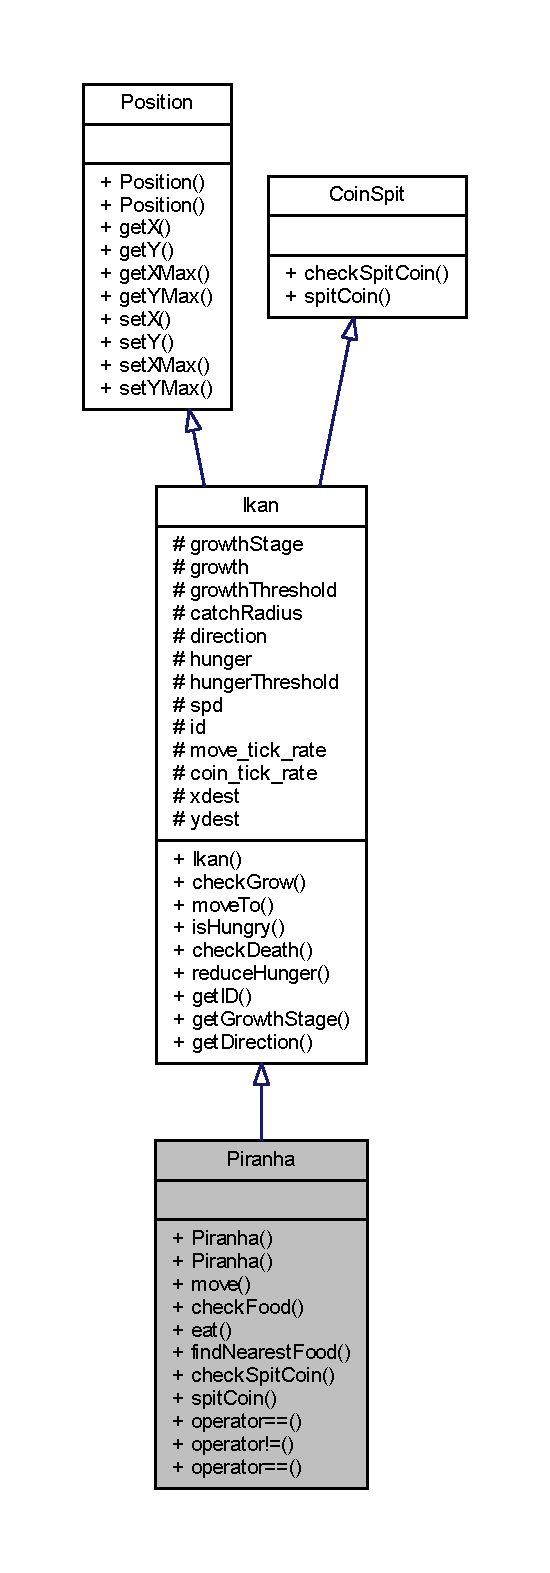
\includegraphics[height=550pt]{class_piranha__inherit__graph}
\end{center}
\end{figure}


Collaboration diagram for Piranha\+:
\nopagebreak
\begin{figure}[H]
\begin{center}
\leavevmode
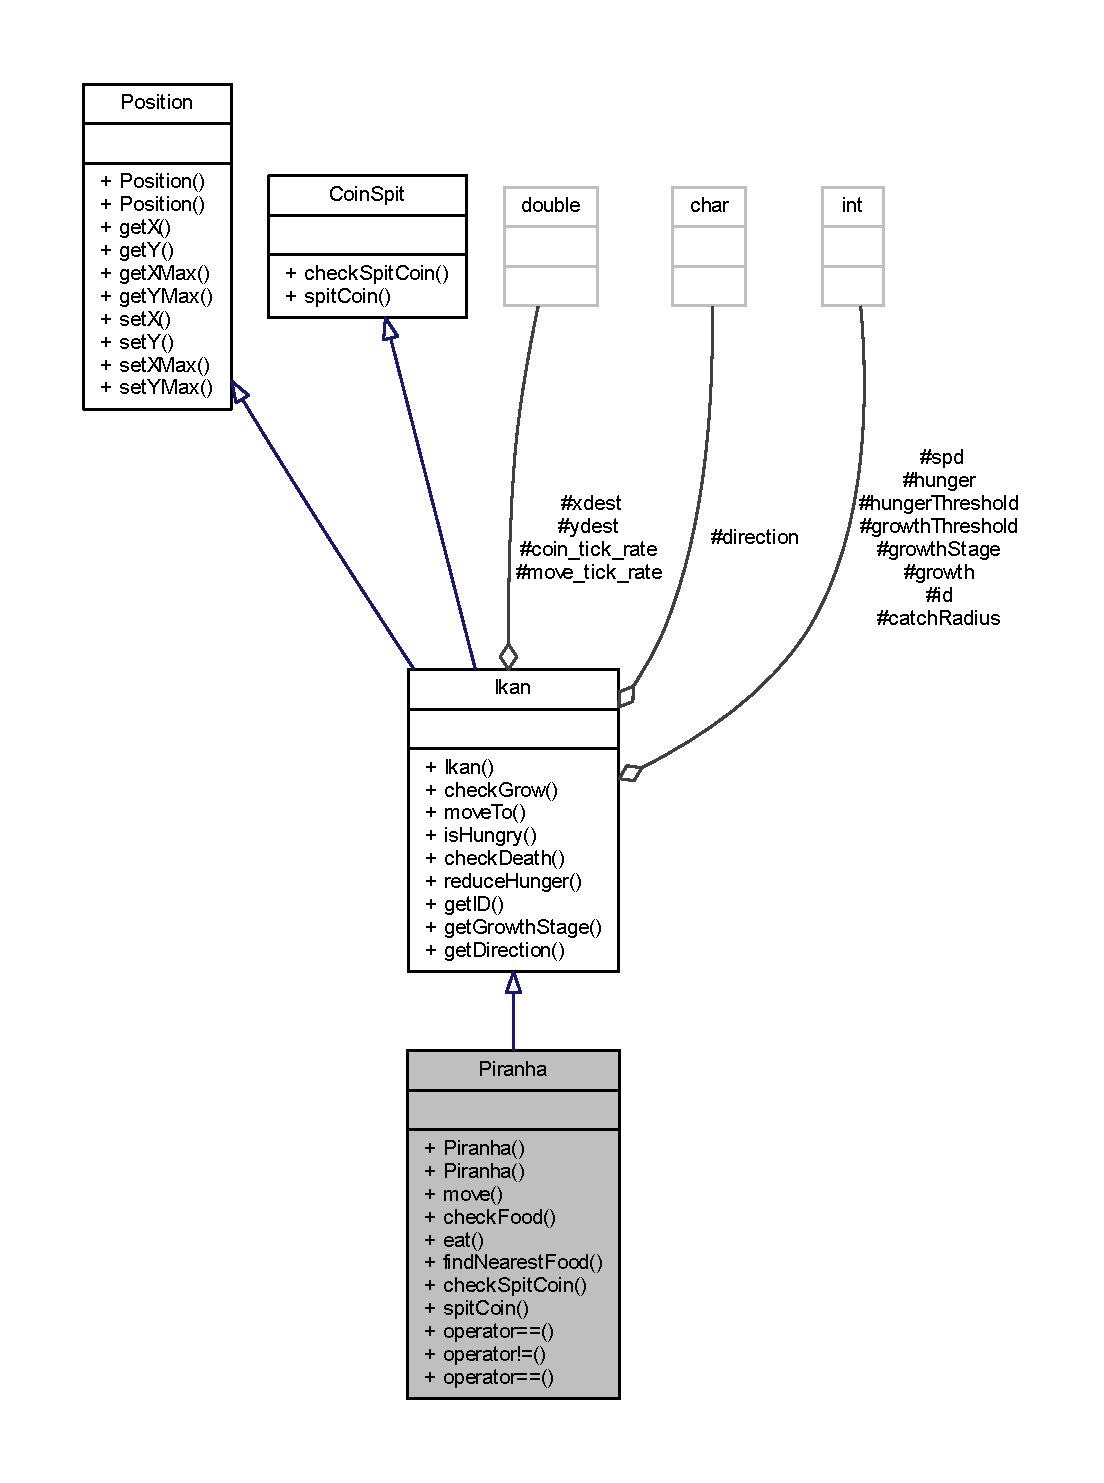
\includegraphics[width=350pt]{class_piranha__coll__graph}
\end{center}
\end{figure}
\subsection*{Public Member Functions}
\begin{DoxyCompactItemize}
\item 
\mbox{\hyperlink{class_piranha_a7e3a4c5c7f458c16717c8cb997fc0331}{Piranha}} ()
\item 
\mbox{\hyperlink{class_piranha_a6ec745c27969134e5a2e4b07ed53d005}{Piranha}} (int x, int y, int xmax, int ymax)
\item 
void \mbox{\hyperlink{class_piranha_a541bc2d7d15271685dd138e0efd45d85}{move}} (\mbox{\hyperlink{class_list}{List}}$<$ \mbox{\hyperlink{class_guppy}{Guppy}} $>$ \&guppy, \mbox{\hyperlink{class_list}{List}}$<$ \mbox{\hyperlink{class_coin}{Coin}} $>$ \&coin, double sec\+\_\+since\+\_\+last)
\item 
bool \mbox{\hyperlink{class_piranha_ad7ead5c0a240432a18657b1415cadde0}{check\+Food}} (\mbox{\hyperlink{class_list}{List}}$<$ \mbox{\hyperlink{class_guppy}{Guppy}} $>$ \&guppy)
\item 
int \mbox{\hyperlink{class_piranha_ab7d97cc3807c53205937ad830f43e3bb}{eat}} (\mbox{\hyperlink{class_list}{List}}$<$ \mbox{\hyperlink{class_guppy}{Guppy}} $>$ \&guppy)
\item 
\mbox{\hyperlink{class_guppy}{Guppy}} $\ast$ \mbox{\hyperlink{class_piranha_a8f8e2a2d3e0ff7a0c712cf78ca578fa8}{find\+Nearest\+Food}} (\mbox{\hyperlink{class_list}{List}}$<$ \mbox{\hyperlink{class_guppy}{Guppy}} $>$ \&guppy)
\item 
bool \mbox{\hyperlink{class_piranha_a9db3ab2f9933739f5744e881f9ee386e}{check\+Spit\+Coin}} ()
\item 
void \mbox{\hyperlink{class_piranha_a4c1c29b2e68b4cb6eb2a295af74bf291}{spit\+Coin}} (\mbox{\hyperlink{class_list}{List}}$<$ \mbox{\hyperlink{class_coin}{Coin}} $>$ \&Lcoin, int value)
\item 
bool \mbox{\hyperlink{class_piranha_aa3789de8579639dcf38cde05b6869859}{operator==}} (const \mbox{\hyperlink{class_piranha}{Piranha}} \&P)
\item 
bool \mbox{\hyperlink{class_piranha_ab6eac12e7a9d9ce9243a16aebc8c9785}{operator!=}} (const \mbox{\hyperlink{class_piranha}{Piranha}} \&P)
\item 
bool \mbox{\hyperlink{class_piranha_a848b090631fa9bf1219ee1c925246125}{operator==}} (std\+::nullptr\+\_\+t n)
\end{DoxyCompactItemize}
\subsection*{Additional Inherited Members}


\subsection{Constructor \& Destructor Documentation}
\mbox{\Hypertarget{class_piranha_a7e3a4c5c7f458c16717c8cb997fc0331}\label{class_piranha_a7e3a4c5c7f458c16717c8cb997fc0331}} 
\index{Piranha@{Piranha}!Piranha@{Piranha}}
\index{Piranha@{Piranha}!Piranha@{Piranha}}
\subsubsection{\texorpdfstring{Piranha()}{Piranha()}\hspace{0.1cm}{\footnotesize\ttfamily [1/2]}}
{\footnotesize\ttfamily Piranha\+::\+Piranha (\begin{DoxyParamCaption}{ }\end{DoxyParamCaption})}

\mbox{\Hypertarget{class_piranha_a6ec745c27969134e5a2e4b07ed53d005}\label{class_piranha_a6ec745c27969134e5a2e4b07ed53d005}} 
\index{Piranha@{Piranha}!Piranha@{Piranha}}
\index{Piranha@{Piranha}!Piranha@{Piranha}}
\subsubsection{\texorpdfstring{Piranha()}{Piranha()}\hspace{0.1cm}{\footnotesize\ttfamily [2/2]}}
{\footnotesize\ttfamily Piranha\+::\+Piranha (\begin{DoxyParamCaption}\item[{int}]{x,  }\item[{int}]{y,  }\item[{int}]{xmax,  }\item[{int}]{ymax }\end{DoxyParamCaption})}



\subsection{Member Function Documentation}
\mbox{\Hypertarget{class_piranha_ad7ead5c0a240432a18657b1415cadde0}\label{class_piranha_ad7ead5c0a240432a18657b1415cadde0}} 
\index{Piranha@{Piranha}!check\+Food@{check\+Food}}
\index{check\+Food@{check\+Food}!Piranha@{Piranha}}
\subsubsection{\texorpdfstring{check\+Food()}{checkFood()}}
{\footnotesize\ttfamily bool Piranha\+::check\+Food (\begin{DoxyParamCaption}\item[{\mbox{\hyperlink{class_list}{List}}$<$ \mbox{\hyperlink{class_guppy}{Guppy}} $>$ \&}]{guppy }\end{DoxyParamCaption})}

\mbox{\Hypertarget{class_piranha_a9db3ab2f9933739f5744e881f9ee386e}\label{class_piranha_a9db3ab2f9933739f5744e881f9ee386e}} 
\index{Piranha@{Piranha}!check\+Spit\+Coin@{check\+Spit\+Coin}}
\index{check\+Spit\+Coin@{check\+Spit\+Coin}!Piranha@{Piranha}}
\subsubsection{\texorpdfstring{check\+Spit\+Coin()}{checkSpitCoin()}}
{\footnotesize\ttfamily bool Piranha\+::check\+Spit\+Coin (\begin{DoxyParamCaption}{ }\end{DoxyParamCaption})\hspace{0.3cm}{\ttfamily [virtual]}}



Implements \mbox{\hyperlink{class_coin_spit_a9471108f825dc67a35ac1a35444b84fd}{Coin\+Spit}}.

\mbox{\Hypertarget{class_piranha_ab7d97cc3807c53205937ad830f43e3bb}\label{class_piranha_ab7d97cc3807c53205937ad830f43e3bb}} 
\index{Piranha@{Piranha}!eat@{eat}}
\index{eat@{eat}!Piranha@{Piranha}}
\subsubsection{\texorpdfstring{eat()}{eat()}}
{\footnotesize\ttfamily int Piranha\+::eat (\begin{DoxyParamCaption}\item[{\mbox{\hyperlink{class_list}{List}}$<$ \mbox{\hyperlink{class_guppy}{Guppy}} $>$ \&}]{guppy }\end{DoxyParamCaption})}

\mbox{\Hypertarget{class_piranha_a8f8e2a2d3e0ff7a0c712cf78ca578fa8}\label{class_piranha_a8f8e2a2d3e0ff7a0c712cf78ca578fa8}} 
\index{Piranha@{Piranha}!find\+Nearest\+Food@{find\+Nearest\+Food}}
\index{find\+Nearest\+Food@{find\+Nearest\+Food}!Piranha@{Piranha}}
\subsubsection{\texorpdfstring{find\+Nearest\+Food()}{findNearestFood()}}
{\footnotesize\ttfamily \mbox{\hyperlink{class_guppy}{Guppy}} $\ast$ Piranha\+::find\+Nearest\+Food (\begin{DoxyParamCaption}\item[{\mbox{\hyperlink{class_list}{List}}$<$ \mbox{\hyperlink{class_guppy}{Guppy}} $>$ \&}]{guppy }\end{DoxyParamCaption})}

\mbox{\Hypertarget{class_piranha_a541bc2d7d15271685dd138e0efd45d85}\label{class_piranha_a541bc2d7d15271685dd138e0efd45d85}} 
\index{Piranha@{Piranha}!move@{move}}
\index{move@{move}!Piranha@{Piranha}}
\subsubsection{\texorpdfstring{move()}{move()}}
{\footnotesize\ttfamily void Piranha\+::move (\begin{DoxyParamCaption}\item[{\mbox{\hyperlink{class_list}{List}}$<$ \mbox{\hyperlink{class_guppy}{Guppy}} $>$ \&}]{guppy,  }\item[{\mbox{\hyperlink{class_list}{List}}$<$ \mbox{\hyperlink{class_coin}{Coin}} $>$ \&}]{coin,  }\item[{double}]{sec\+\_\+since\+\_\+last }\end{DoxyParamCaption})}

\mbox{\Hypertarget{class_piranha_ab6eac12e7a9d9ce9243a16aebc8c9785}\label{class_piranha_ab6eac12e7a9d9ce9243a16aebc8c9785}} 
\index{Piranha@{Piranha}!operator"!=@{operator"!=}}
\index{operator"!=@{operator"!=}!Piranha@{Piranha}}
\subsubsection{\texorpdfstring{operator"!=()}{operator!=()}}
{\footnotesize\ttfamily bool Piranha\+::operator!= (\begin{DoxyParamCaption}\item[{const \mbox{\hyperlink{class_piranha}{Piranha}} \&}]{P }\end{DoxyParamCaption})}

\mbox{\Hypertarget{class_piranha_aa3789de8579639dcf38cde05b6869859}\label{class_piranha_aa3789de8579639dcf38cde05b6869859}} 
\index{Piranha@{Piranha}!operator==@{operator==}}
\index{operator==@{operator==}!Piranha@{Piranha}}
\subsubsection{\texorpdfstring{operator==()}{operator==()}\hspace{0.1cm}{\footnotesize\ttfamily [1/2]}}
{\footnotesize\ttfamily bool Piranha\+::operator== (\begin{DoxyParamCaption}\item[{const \mbox{\hyperlink{class_piranha}{Piranha}} \&}]{P }\end{DoxyParamCaption})}

\mbox{\Hypertarget{class_piranha_a848b090631fa9bf1219ee1c925246125}\label{class_piranha_a848b090631fa9bf1219ee1c925246125}} 
\index{Piranha@{Piranha}!operator==@{operator==}}
\index{operator==@{operator==}!Piranha@{Piranha}}
\subsubsection{\texorpdfstring{operator==()}{operator==()}\hspace{0.1cm}{\footnotesize\ttfamily [2/2]}}
{\footnotesize\ttfamily bool Piranha\+::operator== (\begin{DoxyParamCaption}\item[{std\+::nullptr\+\_\+t}]{n }\end{DoxyParamCaption})}

\mbox{\Hypertarget{class_piranha_a4c1c29b2e68b4cb6eb2a295af74bf291}\label{class_piranha_a4c1c29b2e68b4cb6eb2a295af74bf291}} 
\index{Piranha@{Piranha}!spit\+Coin@{spit\+Coin}}
\index{spit\+Coin@{spit\+Coin}!Piranha@{Piranha}}
\subsubsection{\texorpdfstring{spit\+Coin()}{spitCoin()}}
{\footnotesize\ttfamily void Piranha\+::spit\+Coin (\begin{DoxyParamCaption}\item[{\mbox{\hyperlink{class_list}{List}}$<$ \mbox{\hyperlink{class_coin}{Coin}} $>$ \&}]{Lcoin,  }\item[{int}]{value }\end{DoxyParamCaption})\hspace{0.3cm}{\ttfamily [virtual]}}



Implements \mbox{\hyperlink{class_coin_spit_a336f45a90c4b0b57017b45a5c68f12a7}{Coin\+Spit}}.



The documentation for this class was generated from the following files\+:\begin{DoxyCompactItemize}
\item 
C\+:/\+Users/user/\+Desktop/technical stuff/cpp/\+Tubes O\+O\+P/\+Main Folder/headers/\mbox{\hyperlink{_piranha_8hpp}{Piranha.\+hpp}}\item 
C\+:/\+Users/user/\+Desktop/technical stuff/cpp/\+Tubes O\+O\+P/\+Main Folder/src/\mbox{\hyperlink{_piranha_8cpp}{Piranha.\+cpp}}\end{DoxyCompactItemize}

\hypertarget{class_position}{}\section{Position Class Reference}
\label{class_position}\index{Position@{Position}}


{\ttfamily \#include $<$Position.\+hpp$>$}



Inheritance diagram for Position\+:
\nopagebreak
\begin{figure}[H]
\begin{center}
\leavevmode
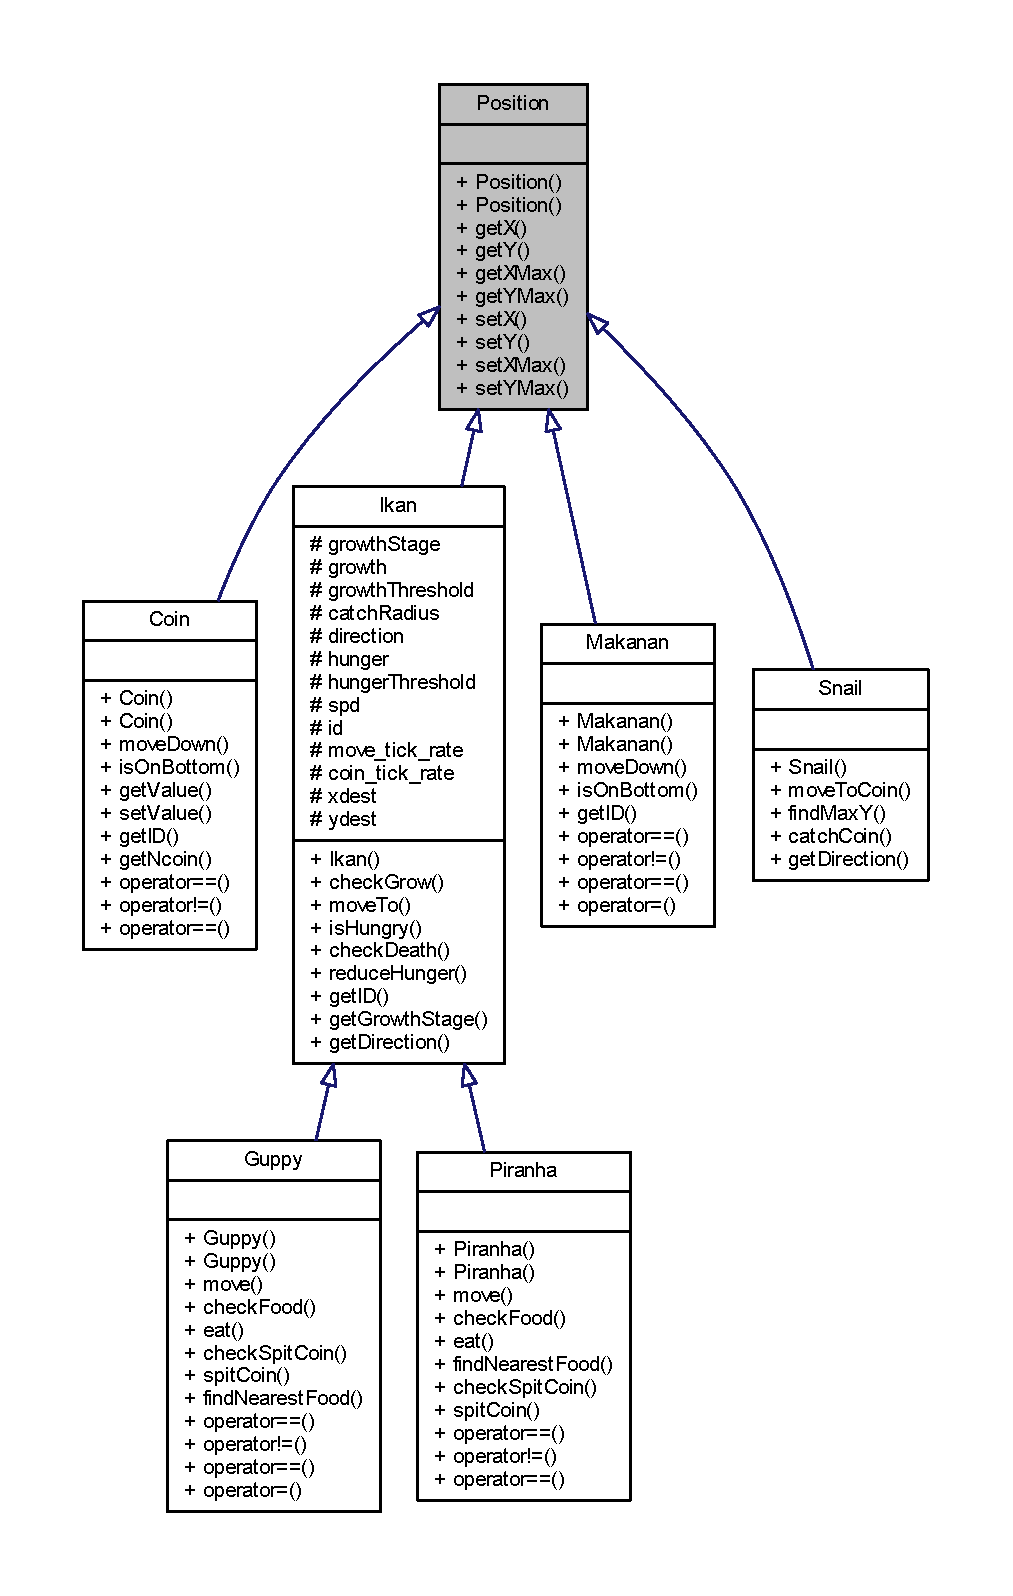
\includegraphics[height=550pt]{class_position__inherit__graph}
\end{center}
\end{figure}


Collaboration diagram for Position\+:
\nopagebreak
\begin{figure}[H]
\begin{center}
\leavevmode
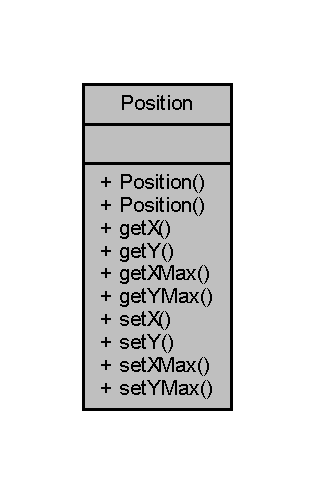
\includegraphics[width=151pt]{class_position__coll__graph}
\end{center}
\end{figure}
\subsection*{Public Member Functions}
\begin{DoxyCompactItemize}
\item 
\mbox{\hyperlink{class_position_a64f68cd96fa0eedccbb760143b82442a}{Position}} (int x\+Max\+Pos, int y\+Max\+Pos)
\item 
\mbox{\hyperlink{class_position_ace954f29b47b5324517ea8ed2487c949}{Position}} (double x, double y, int x\+Max\+Pos, int y\+Max\+Pos)
\item 
double \mbox{\hyperlink{class_position_a10a2a09ec64310f42138f98238ec5fbd}{getX}} () const
\item 
double \mbox{\hyperlink{class_position_a83ae4a9db1a4f29e5a43e5592b65f095}{getY}} () const
\item 
int \mbox{\hyperlink{class_position_abc0b7856e25fab037f1dbfb543ec96cf}{get\+X\+Max}} () const
\item 
int \mbox{\hyperlink{class_position_a6796150fb51e6d8760a5d025b09d1ca5}{get\+Y\+Max}} () const
\item 
void \mbox{\hyperlink{class_position_af12bdfae6a9ccecfc31d968de3613a1d}{setX}} (double x)
\item 
void \mbox{\hyperlink{class_position_a5fbae78d4986da56edad357a82e1e376}{setY}} (double y)
\item 
void \mbox{\hyperlink{class_position_acb2c50493422d1a6faceb3ed7e2a8caf}{set\+X\+Max}} (int x\+Max)
\item 
void \mbox{\hyperlink{class_position_a715321d96c4195ddb3381b52a6cf547c}{set\+Y\+Max}} (int y\+Max)
\end{DoxyCompactItemize}


\subsection{Constructor \& Destructor Documentation}
\mbox{\Hypertarget{class_position_a64f68cd96fa0eedccbb760143b82442a}\label{class_position_a64f68cd96fa0eedccbb760143b82442a}} 
\index{Position@{Position}!Position@{Position}}
\index{Position@{Position}!Position@{Position}}
\subsubsection{\texorpdfstring{Position()}{Position()}\hspace{0.1cm}{\footnotesize\ttfamily [1/2]}}
{\footnotesize\ttfamily Position\+::\+Position (\begin{DoxyParamCaption}\item[{int}]{x\+Max\+Pos,  }\item[{int}]{y\+Max\+Pos }\end{DoxyParamCaption})}

\mbox{\Hypertarget{class_position_ace954f29b47b5324517ea8ed2487c949}\label{class_position_ace954f29b47b5324517ea8ed2487c949}} 
\index{Position@{Position}!Position@{Position}}
\index{Position@{Position}!Position@{Position}}
\subsubsection{\texorpdfstring{Position()}{Position()}\hspace{0.1cm}{\footnotesize\ttfamily [2/2]}}
{\footnotesize\ttfamily Position\+::\+Position (\begin{DoxyParamCaption}\item[{double}]{x,  }\item[{double}]{y,  }\item[{int}]{x\+Max\+Pos,  }\item[{int}]{y\+Max\+Pos }\end{DoxyParamCaption})}



\subsection{Member Function Documentation}
\mbox{\Hypertarget{class_position_a10a2a09ec64310f42138f98238ec5fbd}\label{class_position_a10a2a09ec64310f42138f98238ec5fbd}} 
\index{Position@{Position}!getX@{getX}}
\index{getX@{getX}!Position@{Position}}
\subsubsection{\texorpdfstring{get\+X()}{getX()}}
{\footnotesize\ttfamily double Position\+::getX (\begin{DoxyParamCaption}{ }\end{DoxyParamCaption}) const}

\mbox{\Hypertarget{class_position_abc0b7856e25fab037f1dbfb543ec96cf}\label{class_position_abc0b7856e25fab037f1dbfb543ec96cf}} 
\index{Position@{Position}!get\+X\+Max@{get\+X\+Max}}
\index{get\+X\+Max@{get\+X\+Max}!Position@{Position}}
\subsubsection{\texorpdfstring{get\+X\+Max()}{getXMax()}}
{\footnotesize\ttfamily int Position\+::get\+X\+Max (\begin{DoxyParamCaption}{ }\end{DoxyParamCaption}) const}

\mbox{\Hypertarget{class_position_a83ae4a9db1a4f29e5a43e5592b65f095}\label{class_position_a83ae4a9db1a4f29e5a43e5592b65f095}} 
\index{Position@{Position}!getY@{getY}}
\index{getY@{getY}!Position@{Position}}
\subsubsection{\texorpdfstring{get\+Y()}{getY()}}
{\footnotesize\ttfamily double Position\+::getY (\begin{DoxyParamCaption}{ }\end{DoxyParamCaption}) const}

\mbox{\Hypertarget{class_position_a6796150fb51e6d8760a5d025b09d1ca5}\label{class_position_a6796150fb51e6d8760a5d025b09d1ca5}} 
\index{Position@{Position}!get\+Y\+Max@{get\+Y\+Max}}
\index{get\+Y\+Max@{get\+Y\+Max}!Position@{Position}}
\subsubsection{\texorpdfstring{get\+Y\+Max()}{getYMax()}}
{\footnotesize\ttfamily int Position\+::get\+Y\+Max (\begin{DoxyParamCaption}{ }\end{DoxyParamCaption}) const}

\mbox{\Hypertarget{class_position_af12bdfae6a9ccecfc31d968de3613a1d}\label{class_position_af12bdfae6a9ccecfc31d968de3613a1d}} 
\index{Position@{Position}!setX@{setX}}
\index{setX@{setX}!Position@{Position}}
\subsubsection{\texorpdfstring{set\+X()}{setX()}}
{\footnotesize\ttfamily void Position\+::setX (\begin{DoxyParamCaption}\item[{double}]{x }\end{DoxyParamCaption})}

\mbox{\Hypertarget{class_position_acb2c50493422d1a6faceb3ed7e2a8caf}\label{class_position_acb2c50493422d1a6faceb3ed7e2a8caf}} 
\index{Position@{Position}!set\+X\+Max@{set\+X\+Max}}
\index{set\+X\+Max@{set\+X\+Max}!Position@{Position}}
\subsubsection{\texorpdfstring{set\+X\+Max()}{setXMax()}}
{\footnotesize\ttfamily void Position\+::set\+X\+Max (\begin{DoxyParamCaption}\item[{int}]{x\+Max }\end{DoxyParamCaption})}

\mbox{\Hypertarget{class_position_a5fbae78d4986da56edad357a82e1e376}\label{class_position_a5fbae78d4986da56edad357a82e1e376}} 
\index{Position@{Position}!setY@{setY}}
\index{setY@{setY}!Position@{Position}}
\subsubsection{\texorpdfstring{set\+Y()}{setY()}}
{\footnotesize\ttfamily void Position\+::setY (\begin{DoxyParamCaption}\item[{double}]{y }\end{DoxyParamCaption})}

\mbox{\Hypertarget{class_position_a715321d96c4195ddb3381b52a6cf547c}\label{class_position_a715321d96c4195ddb3381b52a6cf547c}} 
\index{Position@{Position}!set\+Y\+Max@{set\+Y\+Max}}
\index{set\+Y\+Max@{set\+Y\+Max}!Position@{Position}}
\subsubsection{\texorpdfstring{set\+Y\+Max()}{setYMax()}}
{\footnotesize\ttfamily void Position\+::set\+Y\+Max (\begin{DoxyParamCaption}\item[{int}]{y\+Max }\end{DoxyParamCaption})}



The documentation for this class was generated from the following files\+:\begin{DoxyCompactItemize}
\item 
C\+:/\+Users/user/\+Desktop/technical stuff/cpp/\+Tubes O\+O\+P/\+Main Folder/headers/\mbox{\hyperlink{_position_8hpp}{Position.\+hpp}}\item 
C\+:/\+Users/user/\+Desktop/technical stuff/cpp/\+Tubes O\+O\+P/\+Main Folder/src/\mbox{\hyperlink{_position_8cpp}{Position.\+cpp}}\end{DoxyCompactItemize}

\hypertarget{class_snail}{}\section{Snail Class Reference}
\label{class_snail}\index{Snail@{Snail}}


{\ttfamily \#include $<$Snail.\+hpp$>$}



Inheritance diagram for Snail\+:\nopagebreak
\begin{figure}[H]
\begin{center}
\leavevmode
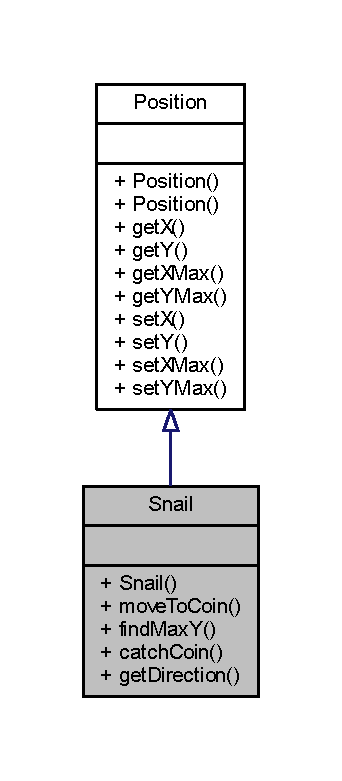
\includegraphics[width=132pt]{class_snail__inherit__graph}
\end{center}
\end{figure}


Collaboration diagram for Snail\+:\nopagebreak
\begin{figure}[H]
\begin{center}
\leavevmode
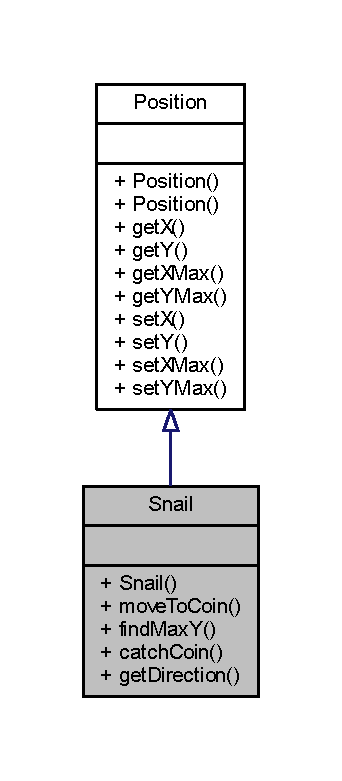
\includegraphics[width=132pt]{class_snail__coll__graph}
\end{center}
\end{figure}
\subsection*{Public Member Functions}
\begin{DoxyCompactItemize}
\item 
\mbox{\hyperlink{class_snail_ad780249a02a8d7a850ccb7255a0cdf14}{Snail}} (int x, int xmax, int ymax)
\item 
int \mbox{\hyperlink{class_snail_ac02f07964ad0a0db28204acc7ed294b7}{move\+To\+Coin}} (\mbox{\hyperlink{class_list}{List}}$<$ \mbox{\hyperlink{class_coin}{Coin}} $>$ \&Lcoin, double sec\+\_\+since\+\_\+last)
\item 
\mbox{\hyperlink{class_coin}{Coin}} $\ast$ \mbox{\hyperlink{class_snail_a1dd9e6d2229dfc452f0163948c7f1980}{find\+MaxY}} (\mbox{\hyperlink{class_list}{List}}$<$ \mbox{\hyperlink{class_coin}{Coin}} $>$ \&Lcoin)
\item 
int \mbox{\hyperlink{class_snail_a2a9deee0c65a5d30f92efd054c6d4155}{catch\+Coin}} (\mbox{\hyperlink{class_list}{List}}$<$ \mbox{\hyperlink{class_coin}{Coin}} $>$ \&Lcoin)
\item 
char \mbox{\hyperlink{class_snail_a5b4774b31b0eb0253910680d4e49f403}{get\+Direction}} ()
\end{DoxyCompactItemize}


\subsection{Constructor \& Destructor Documentation}
\mbox{\Hypertarget{class_snail_ad780249a02a8d7a850ccb7255a0cdf14}\label{class_snail_ad780249a02a8d7a850ccb7255a0cdf14}} 
\index{Snail@{Snail}!Snail@{Snail}}
\index{Snail@{Snail}!Snail@{Snail}}
\subsubsection{\texorpdfstring{Snail()}{Snail()}}
{\footnotesize\ttfamily Snail\+::\+Snail (\begin{DoxyParamCaption}\item[{int}]{x,  }\item[{int}]{xmax,  }\item[{int}]{ymax }\end{DoxyParamCaption})}



\subsection{Member Function Documentation}
\mbox{\Hypertarget{class_snail_a2a9deee0c65a5d30f92efd054c6d4155}\label{class_snail_a2a9deee0c65a5d30f92efd054c6d4155}} 
\index{Snail@{Snail}!catch\+Coin@{catch\+Coin}}
\index{catch\+Coin@{catch\+Coin}!Snail@{Snail}}
\subsubsection{\texorpdfstring{catch\+Coin()}{catchCoin()}}
{\footnotesize\ttfamily int Snail\+::catch\+Coin (\begin{DoxyParamCaption}\item[{\mbox{\hyperlink{class_list}{List}}$<$ \mbox{\hyperlink{class_coin}{Coin}} $>$ \&}]{Lcoin }\end{DoxyParamCaption})}

\mbox{\Hypertarget{class_snail_a1dd9e6d2229dfc452f0163948c7f1980}\label{class_snail_a1dd9e6d2229dfc452f0163948c7f1980}} 
\index{Snail@{Snail}!find\+MaxY@{find\+MaxY}}
\index{find\+MaxY@{find\+MaxY}!Snail@{Snail}}
\subsubsection{\texorpdfstring{find\+Max\+Y()}{findMaxY()}}
{\footnotesize\ttfamily \mbox{\hyperlink{class_coin}{Coin}} $\ast$ Snail\+::find\+MaxY (\begin{DoxyParamCaption}\item[{\mbox{\hyperlink{class_list}{List}}$<$ \mbox{\hyperlink{class_coin}{Coin}} $>$ \&}]{Lcoin }\end{DoxyParamCaption})}

\mbox{\Hypertarget{class_snail_a5b4774b31b0eb0253910680d4e49f403}\label{class_snail_a5b4774b31b0eb0253910680d4e49f403}} 
\index{Snail@{Snail}!get\+Direction@{get\+Direction}}
\index{get\+Direction@{get\+Direction}!Snail@{Snail}}
\subsubsection{\texorpdfstring{get\+Direction()}{getDirection()}}
{\footnotesize\ttfamily char Snail\+::get\+Direction (\begin{DoxyParamCaption}{ }\end{DoxyParamCaption})}

\mbox{\Hypertarget{class_snail_ac02f07964ad0a0db28204acc7ed294b7}\label{class_snail_ac02f07964ad0a0db28204acc7ed294b7}} 
\index{Snail@{Snail}!move\+To\+Coin@{move\+To\+Coin}}
\index{move\+To\+Coin@{move\+To\+Coin}!Snail@{Snail}}
\subsubsection{\texorpdfstring{move\+To\+Coin()}{moveToCoin()}}
{\footnotesize\ttfamily int Snail\+::move\+To\+Coin (\begin{DoxyParamCaption}\item[{\mbox{\hyperlink{class_list}{List}}$<$ \mbox{\hyperlink{class_coin}{Coin}} $>$ \&}]{Lcoin,  }\item[{double}]{sec\+\_\+since\+\_\+last }\end{DoxyParamCaption})}



The documentation for this class was generated from the following files\+:\begin{DoxyCompactItemize}
\item 
headers/\mbox{\hyperlink{_snail_8hpp}{Snail.\+hpp}}\item 
src/\mbox{\hyperlink{_snail_8cpp}{Snail.\+cpp}}\end{DoxyCompactItemize}

\chapter{File Documentation}
\hypertarget{_akuarium_8hpp}{}\section{C\+:/\+Users/user/\+Desktop/technical stuff/cpp/\+Tubes O\+O\+P/\+Main Folder/headers/\+Akuarium.hpp File Reference}
\label{_akuarium_8hpp}\index{C\+:/\+Users/user/\+Desktop/technical stuff/cpp/\+Tubes O\+O\+P/\+Main Folder/headers/\+Akuarium.\+hpp@{C\+:/\+Users/user/\+Desktop/technical stuff/cpp/\+Tubes O\+O\+P/\+Main Folder/headers/\+Akuarium.\+hpp}}
{\ttfamily \#include \char`\"{}List.\+hpp\char`\"{}}\newline
{\ttfamily \#include \char`\"{}Coin.\+hpp\char`\"{}}\newline
{\ttfamily \#include \char`\"{}Guppy.\+hpp\char`\"{}}\newline
{\ttfamily \#include \char`\"{}Piranha.\+hpp\char`\"{}}\newline
{\ttfamily \#include \char`\"{}Makanan.\+hpp\char`\"{}}\newline
{\ttfamily \#include \char`\"{}Snail.\+hpp\char`\"{}}\newline
Include dependency graph for Akuarium.\+hpp\+:
\nopagebreak
\begin{figure}[H]
\begin{center}
\leavevmode
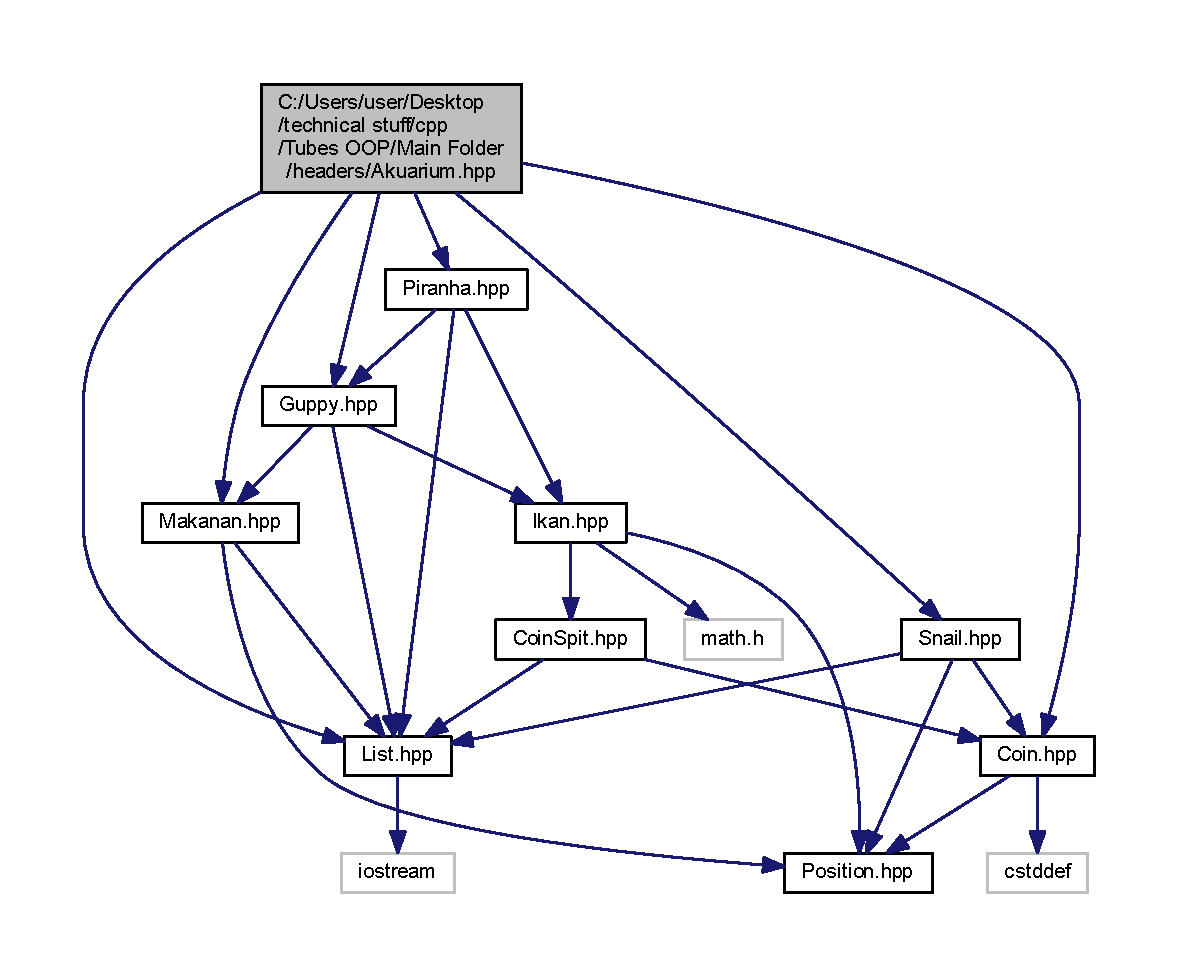
\includegraphics[width=350pt]{_akuarium_8hpp__incl}
\end{center}
\end{figure}
This graph shows which files directly or indirectly include this file\+:
\nopagebreak
\begin{figure}[H]
\begin{center}
\leavevmode
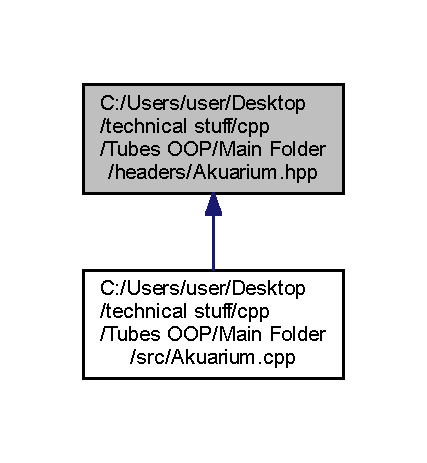
\includegraphics[width=205pt]{_akuarium_8hpp__dep__incl}
\end{center}
\end{figure}
\subsection*{Classes}
\begin{DoxyCompactItemize}
\item 
class \mbox{\hyperlink{class_akuarium}{Akuarium}}
\end{DoxyCompactItemize}

\hypertarget{_coin_8hpp}{}\section{headers/\+Coin.hpp File Reference}
\label{_coin_8hpp}\index{headers/\+Coin.\+hpp@{headers/\+Coin.\+hpp}}
{\ttfamily \#include \char`\"{}Position.\+hpp\char`\"{}}\newline
{\ttfamily \#include $<$cstddef$>$}\newline
Include dependency graph for Coin.\+hpp\+:
\nopagebreak
\begin{figure}[H]
\begin{center}
\leavevmode
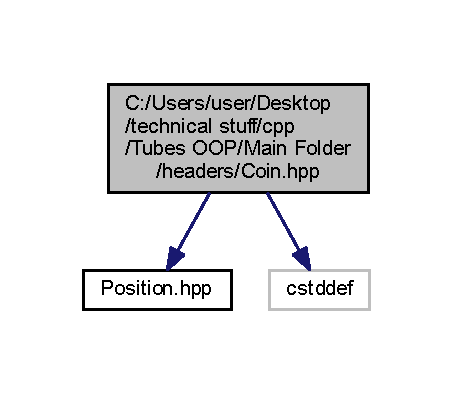
\includegraphics[width=218pt]{_coin_8hpp__incl}
\end{center}
\end{figure}
This graph shows which files directly or indirectly include this file\+:
\nopagebreak
\begin{figure}[H]
\begin{center}
\leavevmode
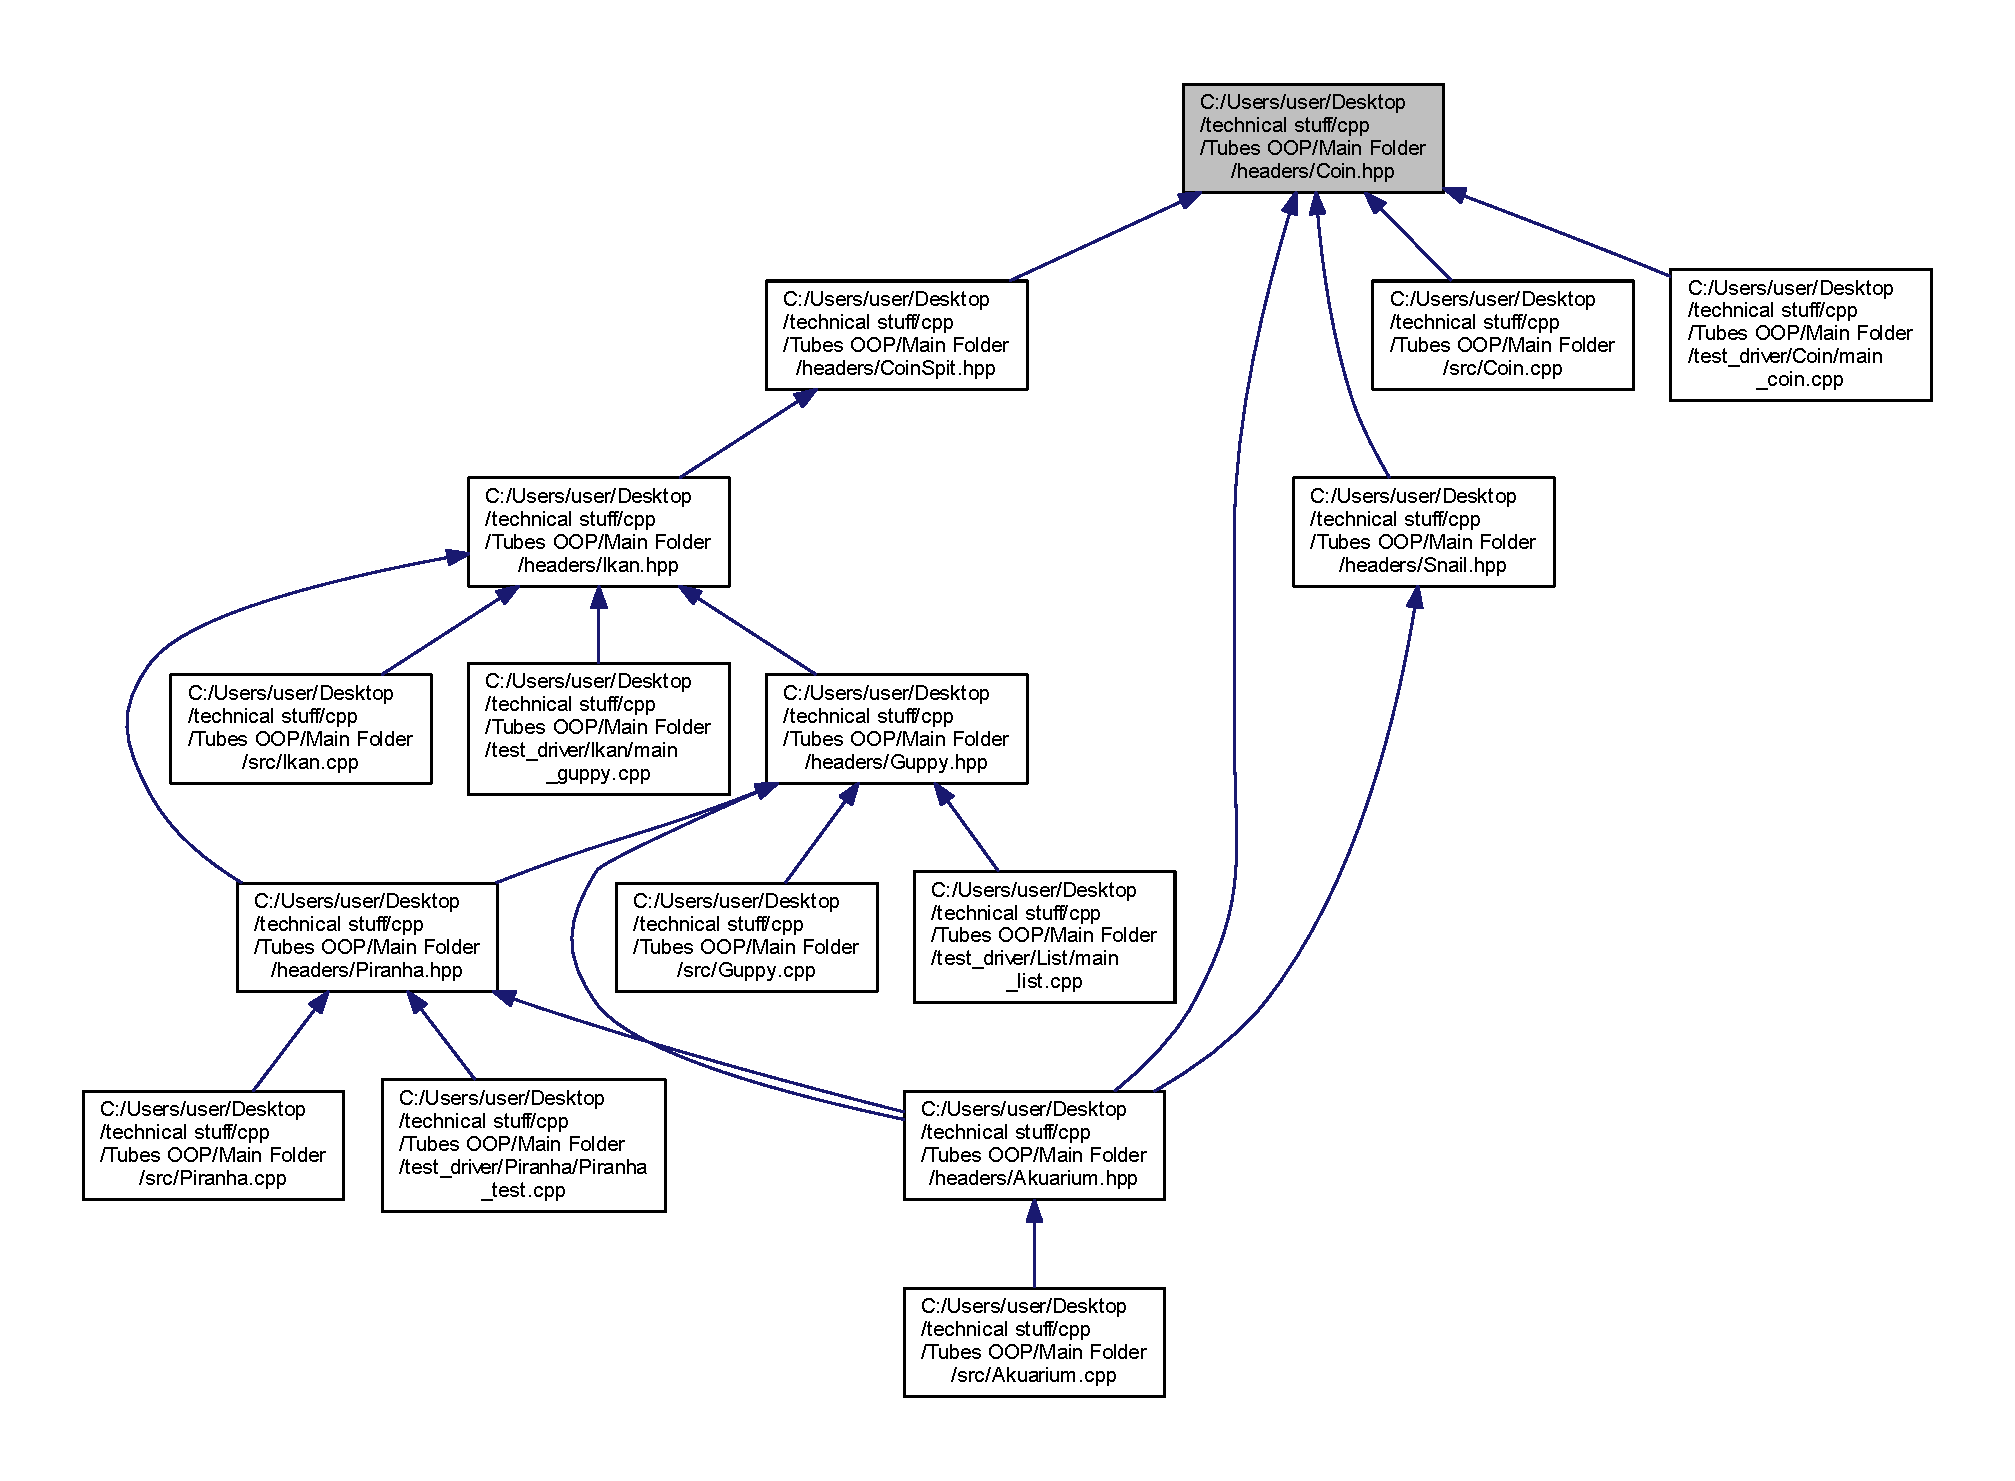
\includegraphics[width=350pt]{_coin_8hpp__dep__incl}
\end{center}
\end{figure}
\subsection*{Classes}
\begin{DoxyCompactItemize}
\item 
class \mbox{\hyperlink{class_coin}{Coin}}
\end{DoxyCompactItemize}

\hypertarget{_coin_spit_8hpp}{}\section{C\+:/\+Users/user/\+Desktop/technical stuff/cpp/\+Tubes O\+O\+P/\+Main Folder/headers/\+Coin\+Spit.hpp File Reference}
\label{_coin_spit_8hpp}\index{C\+:/\+Users/user/\+Desktop/technical stuff/cpp/\+Tubes O\+O\+P/\+Main Folder/headers/\+Coin\+Spit.\+hpp@{C\+:/\+Users/user/\+Desktop/technical stuff/cpp/\+Tubes O\+O\+P/\+Main Folder/headers/\+Coin\+Spit.\+hpp}}
{\ttfamily \#include \char`\"{}List.\+hpp\char`\"{}}\newline
{\ttfamily \#include \char`\"{}Coin.\+hpp\char`\"{}}\newline
Include dependency graph for Coin\+Spit.\+hpp\+:
\nopagebreak
\begin{figure}[H]
\begin{center}
\leavevmode
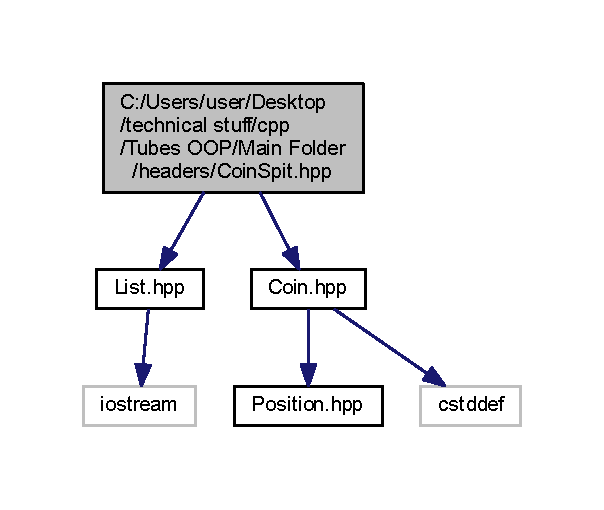
\includegraphics[width=290pt]{_coin_spit_8hpp__incl}
\end{center}
\end{figure}
This graph shows which files directly or indirectly include this file\+:
\nopagebreak
\begin{figure}[H]
\begin{center}
\leavevmode
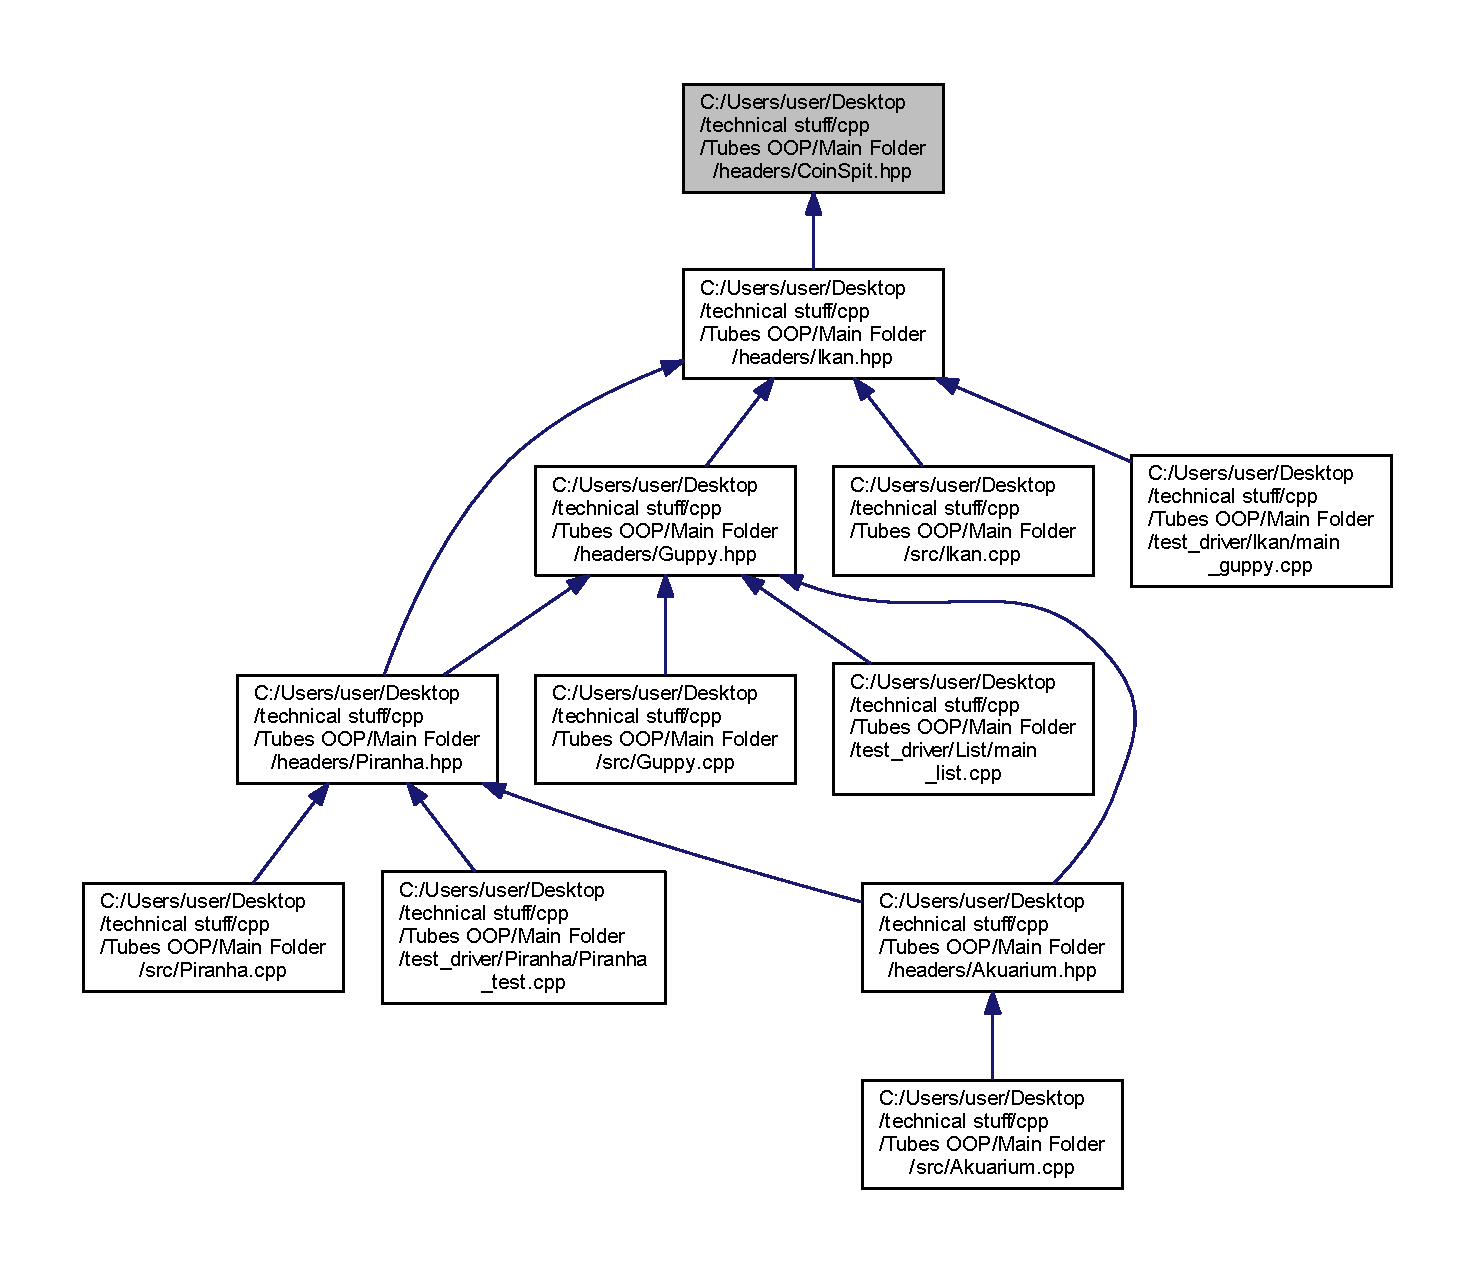
\includegraphics[width=350pt]{_coin_spit_8hpp__dep__incl}
\end{center}
\end{figure}
\subsection*{Classes}
\begin{DoxyCompactItemize}
\item 
class \mbox{\hyperlink{class_coin_spit}{Coin\+Spit}}
\end{DoxyCompactItemize}

\hypertarget{_guppy_8hpp}{}\section{headers/\+Guppy.hpp File Reference}
\label{_guppy_8hpp}\index{headers/\+Guppy.\+hpp@{headers/\+Guppy.\+hpp}}
{\ttfamily \#include \char`\"{}Ikan.\+hpp\char`\"{}}\newline
{\ttfamily \#include \char`\"{}Makanan.\+hpp\char`\"{}}\newline
{\ttfamily \#include \char`\"{}List.\+hpp\char`\"{}}\newline
Include dependency graph for Guppy.\+hpp\+:
\nopagebreak
\begin{figure}[H]
\begin{center}
\leavevmode
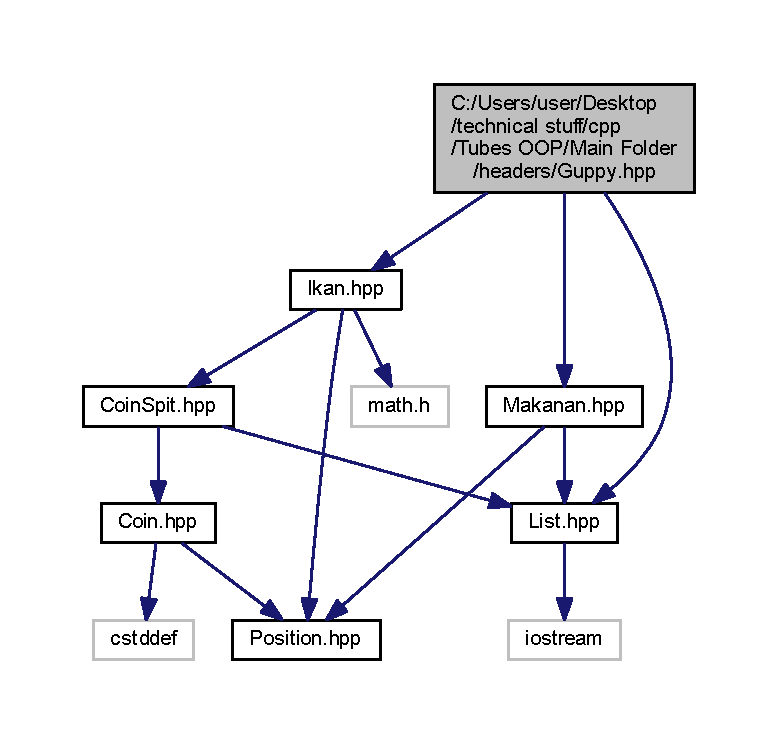
\includegraphics[width=350pt]{_guppy_8hpp__incl}
\end{center}
\end{figure}
This graph shows which files directly or indirectly include this file\+:
\nopagebreak
\begin{figure}[H]
\begin{center}
\leavevmode
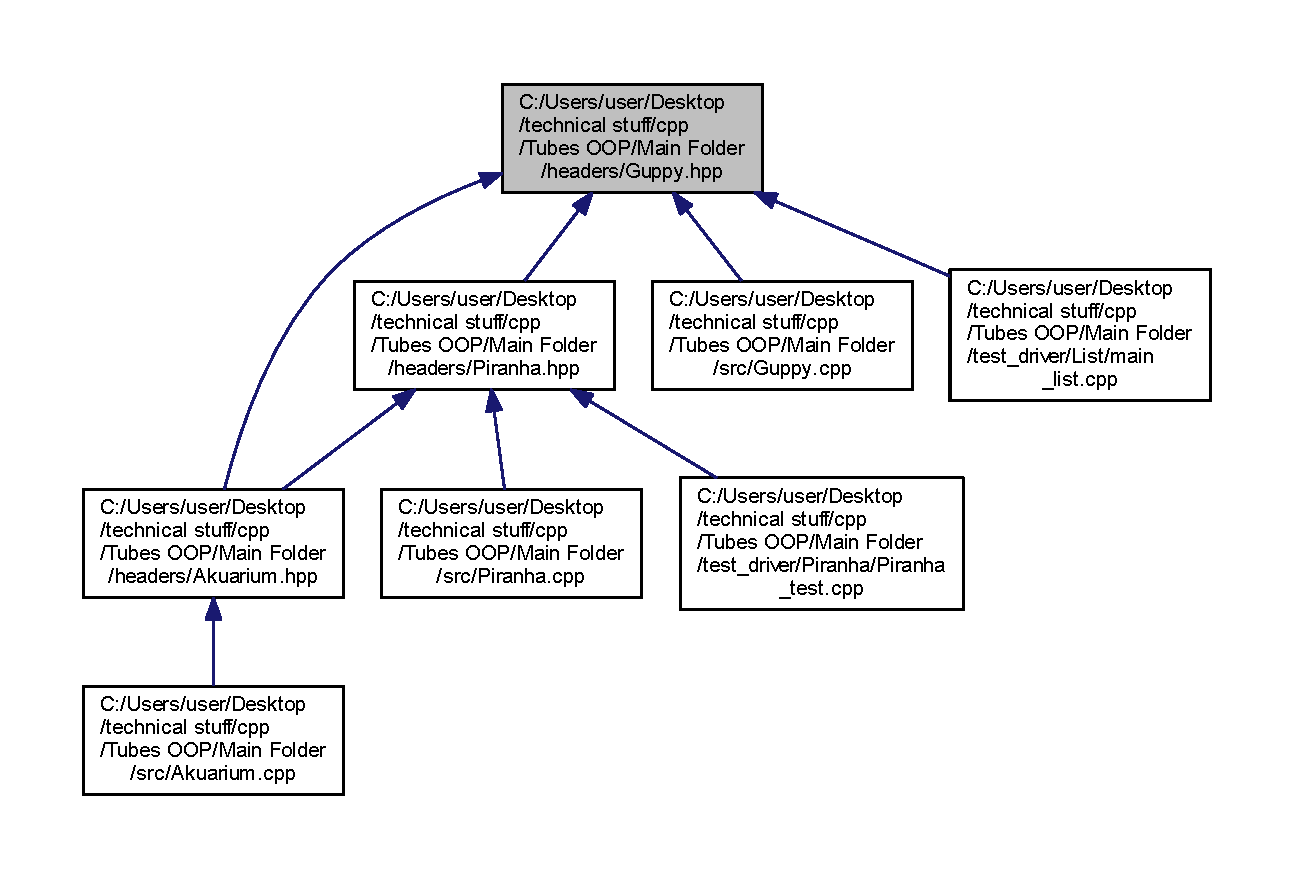
\includegraphics[width=350pt]{_guppy_8hpp__dep__incl}
\end{center}
\end{figure}
\subsection*{Classes}
\begin{DoxyCompactItemize}
\item 
class \mbox{\hyperlink{class_guppy}{Guppy}}
\end{DoxyCompactItemize}

\hypertarget{_ikan_8hpp}{}\section{C\+:/\+Users/user/\+Desktop/technical stuff/cpp/\+Tubes O\+O\+P/\+Main Folder/headers/\+Ikan.hpp File Reference}
\label{_ikan_8hpp}\index{C\+:/\+Users/user/\+Desktop/technical stuff/cpp/\+Tubes O\+O\+P/\+Main Folder/headers/\+Ikan.\+hpp@{C\+:/\+Users/user/\+Desktop/technical stuff/cpp/\+Tubes O\+O\+P/\+Main Folder/headers/\+Ikan.\+hpp}}
{\ttfamily \#include \char`\"{}Position.\+hpp\char`\"{}}\newline
{\ttfamily \#include \char`\"{}Coin\+Spit.\+hpp\char`\"{}}\newline
{\ttfamily \#include $<$math.\+h$>$}\newline
Include dependency graph for Ikan.\+hpp\+:
\nopagebreak
\begin{figure}[H]
\begin{center}
\leavevmode
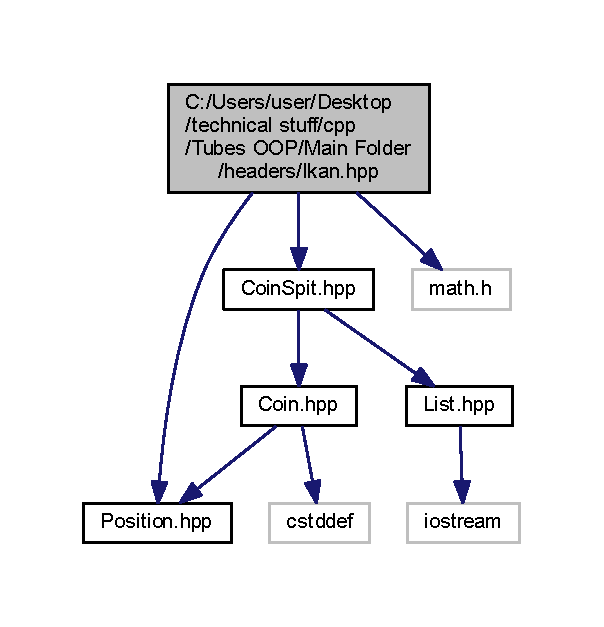
\includegraphics[width=290pt]{_ikan_8hpp__incl}
\end{center}
\end{figure}
This graph shows which files directly or indirectly include this file\+:
\nopagebreak
\begin{figure}[H]
\begin{center}
\leavevmode
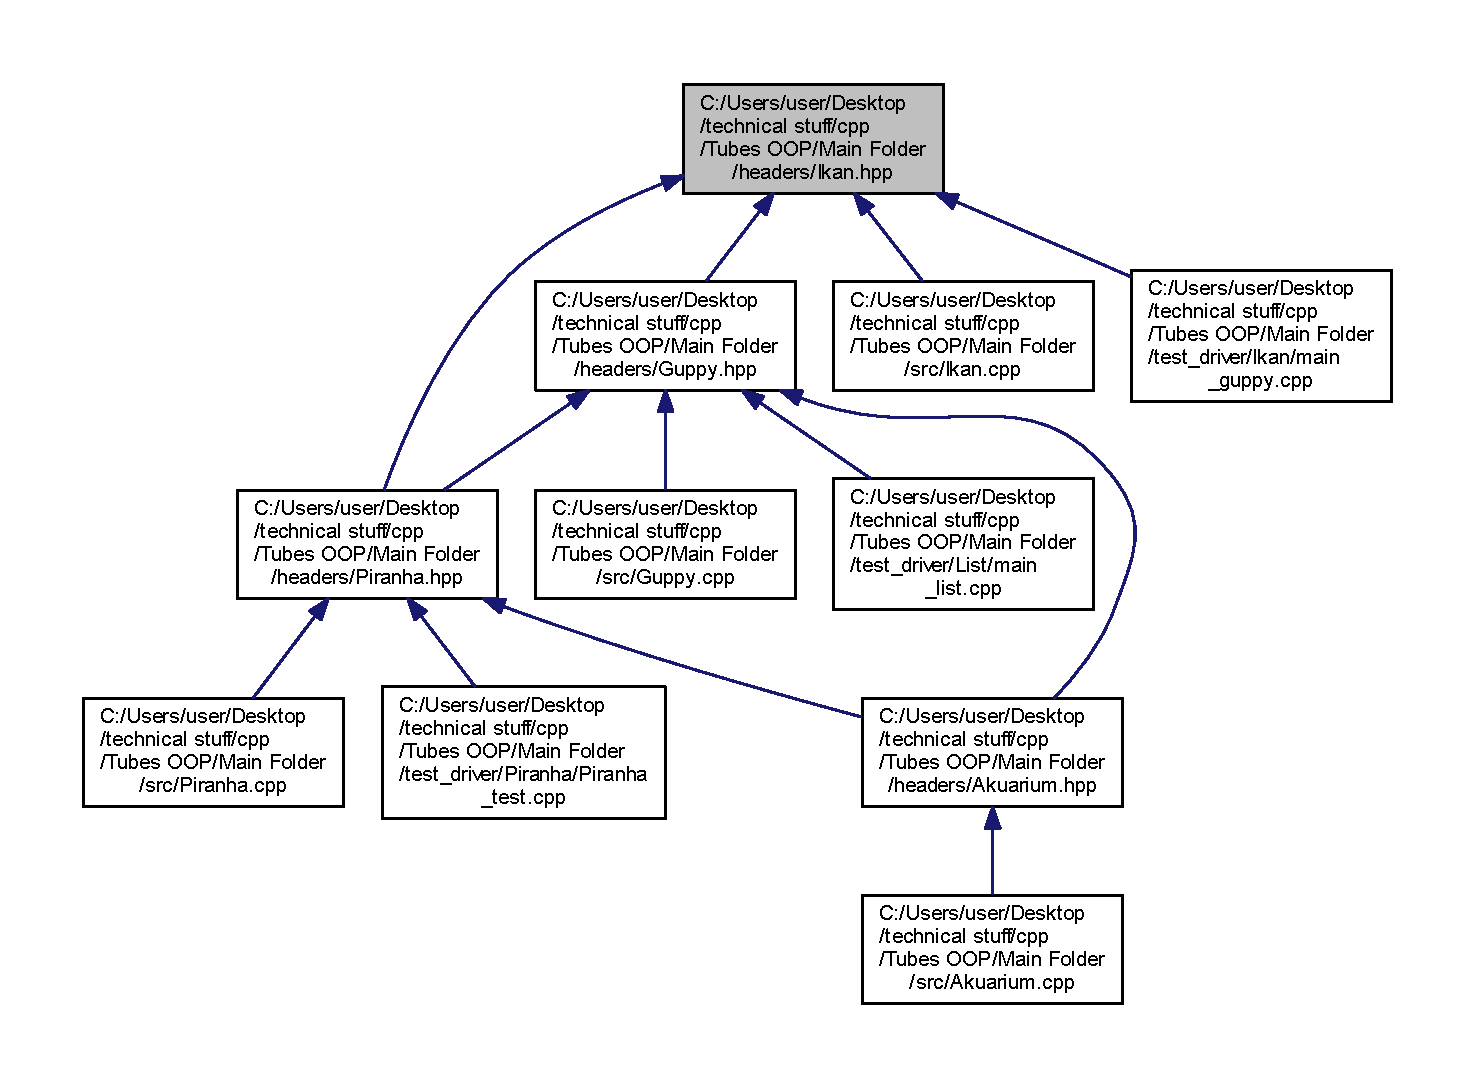
\includegraphics[width=350pt]{_ikan_8hpp__dep__incl}
\end{center}
\end{figure}
\subsection*{Classes}
\begin{DoxyCompactItemize}
\item 
class \mbox{\hyperlink{class_ikan}{Ikan}}
\end{DoxyCompactItemize}

\hypertarget{_list_8hpp}{}\section{headers/\+List.hpp File Reference}
\label{_list_8hpp}\index{headers/\+List.\+hpp@{headers/\+List.\+hpp}}
{\ttfamily \#include $<$iostream$>$}\newline
Include dependency graph for List.\+hpp\+:
\nopagebreak
\begin{figure}[H]
\begin{center}
\leavevmode
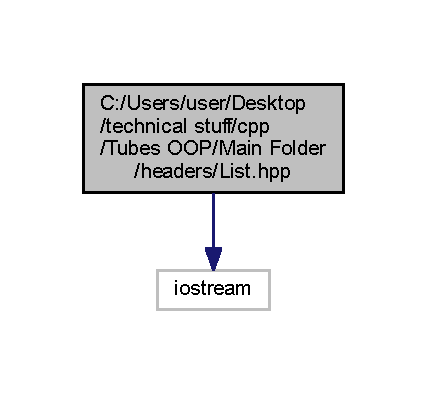
\includegraphics[width=169pt]{_list_8hpp__incl}
\end{center}
\end{figure}
This graph shows which files directly or indirectly include this file\+:
\nopagebreak
\begin{figure}[H]
\begin{center}
\leavevmode
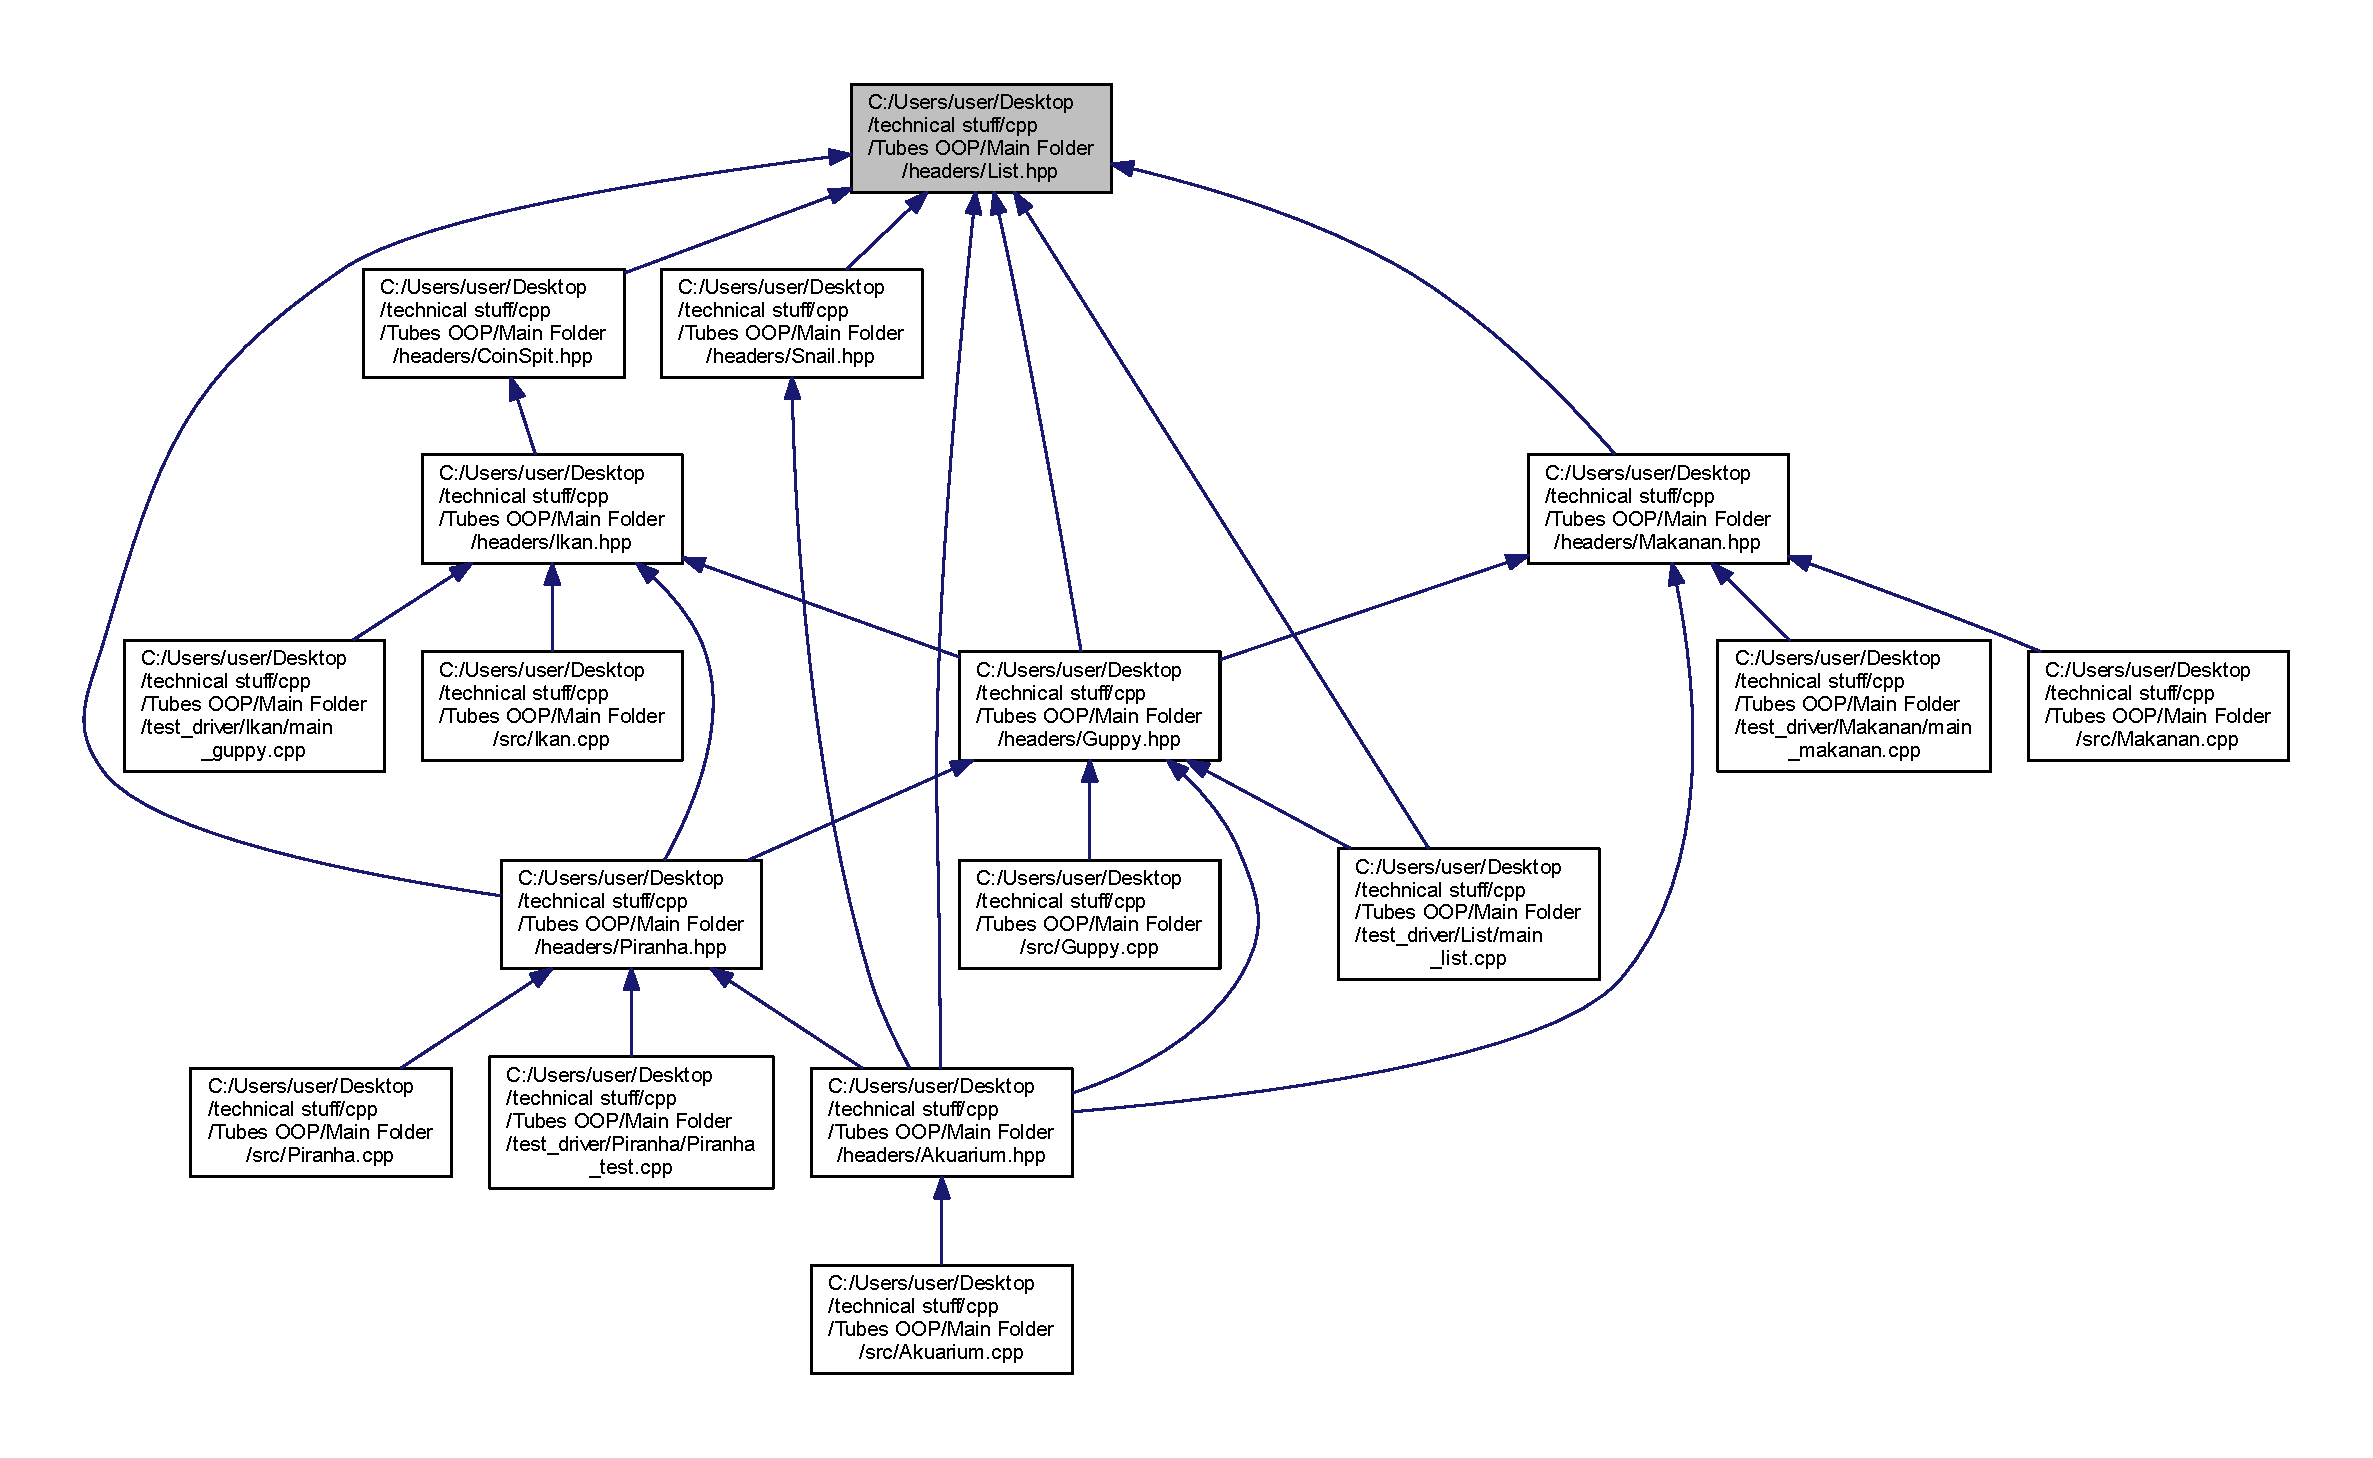
\includegraphics[width=350pt]{_list_8hpp__dep__incl}
\end{center}
\end{figure}
\subsection*{Classes}
\begin{DoxyCompactItemize}
\item 
class \mbox{\hyperlink{class_list}{List$<$ T $>$}}
\end{DoxyCompactItemize}

\hypertarget{_makanan_8hpp}{}\section{headers/\+Makanan.hpp File Reference}
\label{_makanan_8hpp}\index{headers/\+Makanan.\+hpp@{headers/\+Makanan.\+hpp}}
{\ttfamily \#include \char`\"{}Position.\+hpp\char`\"{}}\newline
{\ttfamily \#include \char`\"{}List.\+hpp\char`\"{}}\newline
Include dependency graph for Makanan.\+hpp\+:
\nopagebreak
\begin{figure}[H]
\begin{center}
\leavevmode
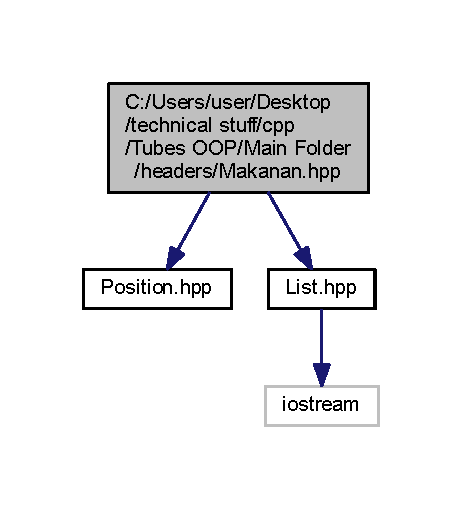
\includegraphics[width=222pt]{_makanan_8hpp__incl}
\end{center}
\end{figure}
This graph shows which files directly or indirectly include this file\+:
\nopagebreak
\begin{figure}[H]
\begin{center}
\leavevmode
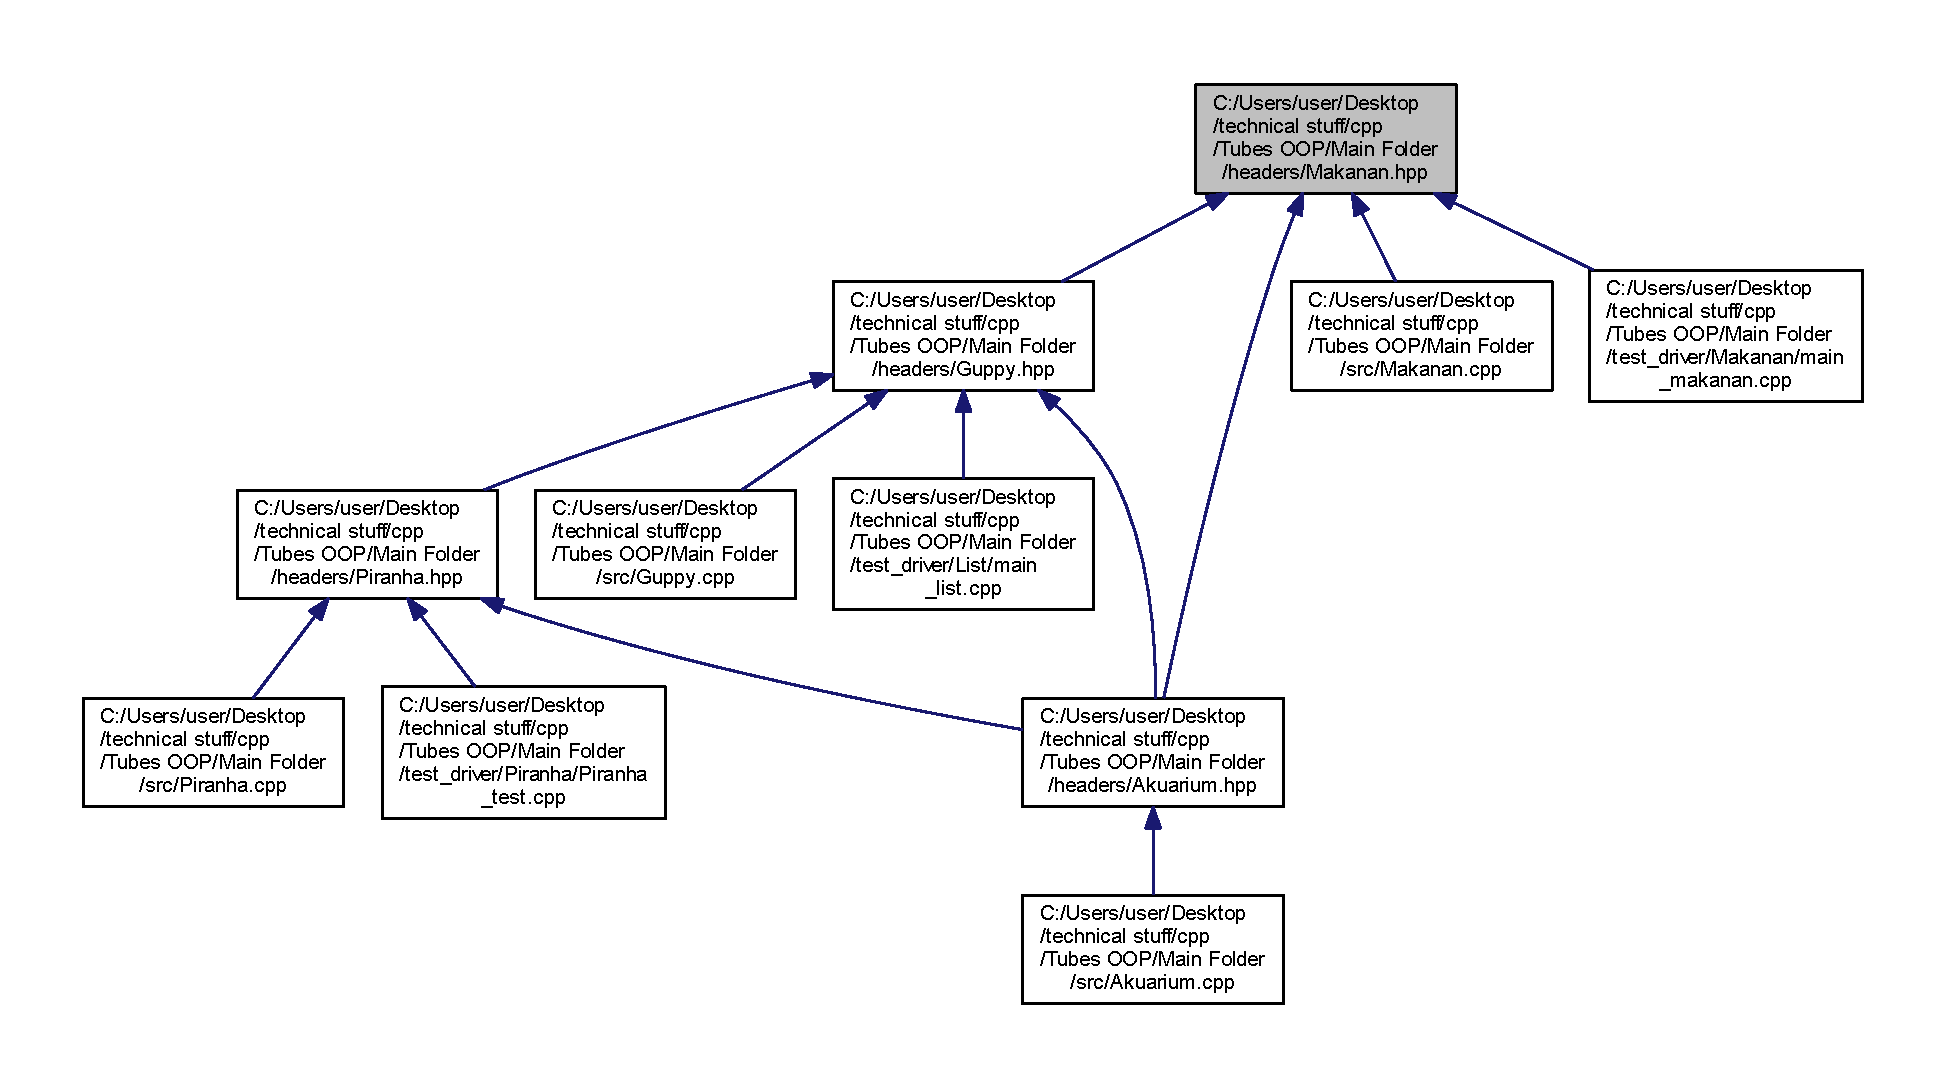
\includegraphics[width=350pt]{_makanan_8hpp__dep__incl}
\end{center}
\end{figure}
\subsection*{Classes}
\begin{DoxyCompactItemize}
\item 
class \mbox{\hyperlink{class_makanan}{Makanan}}
\end{DoxyCompactItemize}

\hypertarget{oop_8hpp}{}\section{headers/oop.hpp File Reference}
\label{oop_8hpp}\index{headers/oop.\+hpp@{headers/oop.\+hpp}}
{\ttfamily \#include $<$S\+D\+L.\+h$>$}\newline
{\ttfamily \#include $<$S\+D\+L\+\_\+image.\+h$>$}\newline
{\ttfamily \#include $<$S\+D\+L\+\_\+ttf.\+h$>$}\newline
{\ttfamily \#include $<$set$>$}\newline
{\ttfamily \#include $<$string$>$}\newline
Include dependency graph for oop.\+hpp\+:
\nopagebreak
\begin{figure}[H]
\begin{center}
\leavevmode
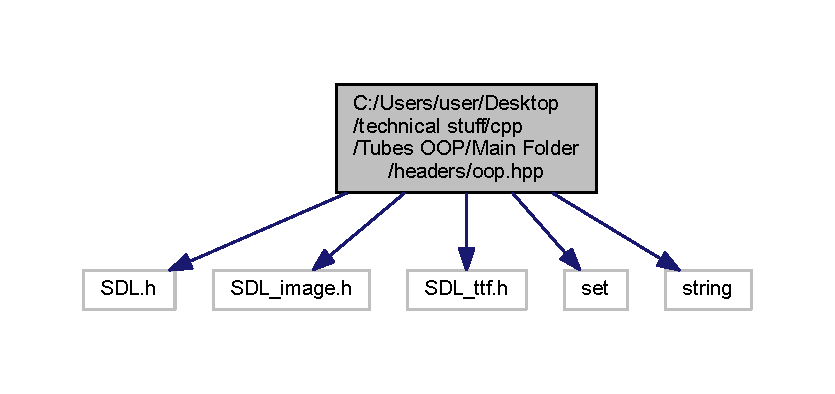
\includegraphics[width=350pt]{oop_8hpp__incl}
\end{center}
\end{figure}
This graph shows which files directly or indirectly include this file\+:
\nopagebreak
\begin{figure}[H]
\begin{center}
\leavevmode
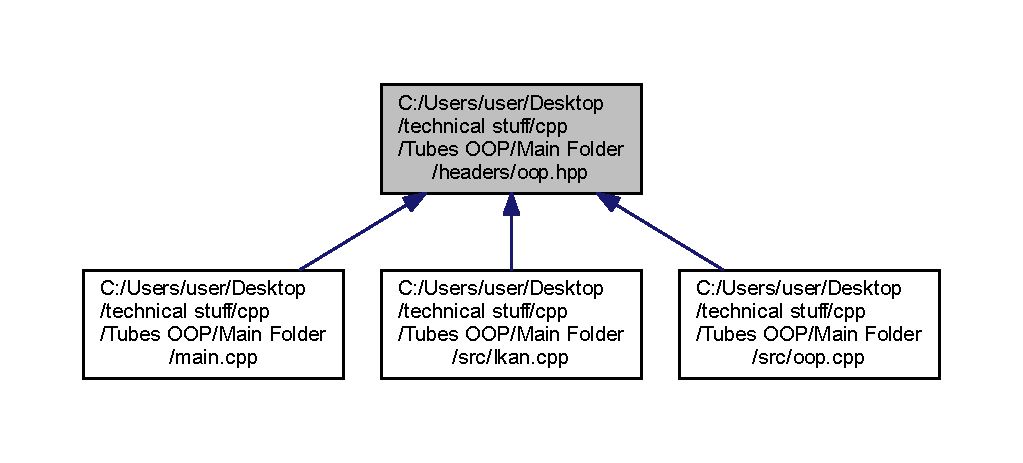
\includegraphics[width=310pt]{oop_8hpp__dep__incl}
\end{center}
\end{figure}
\subsection*{Functions}
\begin{DoxyCompactItemize}
\item 
bool \mbox{\hyperlink{oop_8hpp_aee8048628ff2b5c026c9e15acdcaacb8}{init}} ()
\item 
void \mbox{\hyperlink{oop_8hpp_a5ae591df94fc66ccb85cbb6565368bca}{close}} ()
\item 
void \mbox{\hyperlink{oop_8hpp_a0f01596e4fd0a81c514c706c4936ee8d}{draw\+\_\+image}} (std\+::string filename, int x, int y)
\item 
void \mbox{\hyperlink{oop_8hpp_a2b13ce610f0fb0df7a95eb2307e319d2}{draw\+\_\+text}} (std\+::string text, int font\+\_\+size, int x, int y, unsigned char r, unsigned char g, unsigned char b)
\item 
void \mbox{\hyperlink{oop_8hpp_a4953d1edcbbfc7e420c423ded1d5621a}{clear\+\_\+screen}} ()
\item 
void \mbox{\hyperlink{oop_8hpp_a10da25e92e69613be93d099bb029feb2}{update\+\_\+screen}} ()
\item 
void \mbox{\hyperlink{oop_8hpp_ab19fbad269feb4f8cf725031233ba56e}{handle\+\_\+input}} ()
\item 
bool \mbox{\hyperlink{oop_8hpp_a1b14e3b0f5799f93f8dab7f5c6819298}{quit\+\_\+pressed}} ()
\item 
const std\+::set$<$ S\+D\+L\+\_\+\+Keycode $>$ \& \mbox{\hyperlink{oop_8hpp_a155dba9d2b234776d0fb743da0dcdbc2}{get\+\_\+pressed\+\_\+keys}} ()
\item 
const std\+::set$<$ S\+D\+L\+\_\+\+Keycode $>$ \& \mbox{\hyperlink{oop_8hpp_a4fdfe498ed93ea27801b69f2158e5e6a}{get\+\_\+tapped\+\_\+keys}} ()
\item 
const std\+::set$<$ Uint8 $>$ \& \mbox{\hyperlink{oop_8hpp_a921d1df60af4bfb75d55de50bf6d1e19}{get\+\_\+pressed\+\_\+buttons}} ()
\item 
const std\+::set$<$ Uint8 $>$ \& \mbox{\hyperlink{oop_8hpp_abe85482fb212faff74cb7e33060d2f1d}{get\+\_\+tapped\+\_\+buttons}} ()
\item 
double \mbox{\hyperlink{oop_8hpp_a1ba1773fee3381786a816dc207a1f8d5}{time\+\_\+since\+\_\+start}} ()
\end{DoxyCompactItemize}
\subsection*{Variables}
\begin{DoxyCompactItemize}
\item 
const int \mbox{\hyperlink{oop_8hpp_a3482785bd2a4c8b307f9e0b6f54e2c36}{S\+C\+R\+E\+E\+N\+\_\+\+W\+I\+D\+TH}} = 1280
\item 
const int \mbox{\hyperlink{oop_8hpp_ab454541ae58bcf6555e8d723b1eb95e7}{S\+C\+R\+E\+E\+N\+\_\+\+H\+E\+I\+G\+HT}} = 760
\item 
const char $\ast$const \mbox{\hyperlink{oop_8hpp_aa138e55e1cd5980069d8a26538b96fd3}{F\+O\+N\+T\+\_\+\+N\+A\+ME}} = \char`\"{}resources/helvetica-\/normal.\+ttf\char`\"{}
\end{DoxyCompactItemize}


\subsection{Function Documentation}
\mbox{\Hypertarget{oop_8hpp_a4953d1edcbbfc7e420c423ded1d5621a}\label{oop_8hpp_a4953d1edcbbfc7e420c423ded1d5621a}} 
\index{oop.\+hpp@{oop.\+hpp}!clear\+\_\+screen@{clear\+\_\+screen}}
\index{clear\+\_\+screen@{clear\+\_\+screen}!oop.\+hpp@{oop.\+hpp}}
\subsubsection{\texorpdfstring{clear\+\_\+screen()}{clear\_screen()}}
{\footnotesize\ttfamily void clear\+\_\+screen (\begin{DoxyParamCaption}{ }\end{DoxyParamCaption})}

\mbox{\Hypertarget{oop_8hpp_a5ae591df94fc66ccb85cbb6565368bca}\label{oop_8hpp_a5ae591df94fc66ccb85cbb6565368bca}} 
\index{oop.\+hpp@{oop.\+hpp}!close@{close}}
\index{close@{close}!oop.\+hpp@{oop.\+hpp}}
\subsubsection{\texorpdfstring{close()}{close()}}
{\footnotesize\ttfamily void close (\begin{DoxyParamCaption}{ }\end{DoxyParamCaption})}

\mbox{\Hypertarget{oop_8hpp_a0f01596e4fd0a81c514c706c4936ee8d}\label{oop_8hpp_a0f01596e4fd0a81c514c706c4936ee8d}} 
\index{oop.\+hpp@{oop.\+hpp}!draw\+\_\+image@{draw\+\_\+image}}
\index{draw\+\_\+image@{draw\+\_\+image}!oop.\+hpp@{oop.\+hpp}}
\subsubsection{\texorpdfstring{draw\+\_\+image()}{draw\_image()}}
{\footnotesize\ttfamily void draw\+\_\+image (\begin{DoxyParamCaption}\item[{std\+::string}]{filename,  }\item[{int}]{x,  }\item[{int}]{y }\end{DoxyParamCaption})}

\mbox{\Hypertarget{oop_8hpp_a2b13ce610f0fb0df7a95eb2307e319d2}\label{oop_8hpp_a2b13ce610f0fb0df7a95eb2307e319d2}} 
\index{oop.\+hpp@{oop.\+hpp}!draw\+\_\+text@{draw\+\_\+text}}
\index{draw\+\_\+text@{draw\+\_\+text}!oop.\+hpp@{oop.\+hpp}}
\subsubsection{\texorpdfstring{draw\+\_\+text()}{draw\_text()}}
{\footnotesize\ttfamily void draw\+\_\+text (\begin{DoxyParamCaption}\item[{std\+::string}]{text,  }\item[{int}]{font\+\_\+size,  }\item[{int}]{x,  }\item[{int}]{y,  }\item[{unsigned char}]{r,  }\item[{unsigned char}]{g,  }\item[{unsigned char}]{b }\end{DoxyParamCaption})}

\mbox{\Hypertarget{oop_8hpp_a921d1df60af4bfb75d55de50bf6d1e19}\label{oop_8hpp_a921d1df60af4bfb75d55de50bf6d1e19}} 
\index{oop.\+hpp@{oop.\+hpp}!get\+\_\+pressed\+\_\+buttons@{get\+\_\+pressed\+\_\+buttons}}
\index{get\+\_\+pressed\+\_\+buttons@{get\+\_\+pressed\+\_\+buttons}!oop.\+hpp@{oop.\+hpp}}
\subsubsection{\texorpdfstring{get\+\_\+pressed\+\_\+buttons()}{get\_pressed\_buttons()}}
{\footnotesize\ttfamily const std\+::set$<$Uint8$>$\& get\+\_\+pressed\+\_\+buttons (\begin{DoxyParamCaption}{ }\end{DoxyParamCaption})}

\mbox{\Hypertarget{oop_8hpp_a155dba9d2b234776d0fb743da0dcdbc2}\label{oop_8hpp_a155dba9d2b234776d0fb743da0dcdbc2}} 
\index{oop.\+hpp@{oop.\+hpp}!get\+\_\+pressed\+\_\+keys@{get\+\_\+pressed\+\_\+keys}}
\index{get\+\_\+pressed\+\_\+keys@{get\+\_\+pressed\+\_\+keys}!oop.\+hpp@{oop.\+hpp}}
\subsubsection{\texorpdfstring{get\+\_\+pressed\+\_\+keys()}{get\_pressed\_keys()}}
{\footnotesize\ttfamily const std\+::set$<$S\+D\+L\+\_\+\+Keycode$>$\& get\+\_\+pressed\+\_\+keys (\begin{DoxyParamCaption}{ }\end{DoxyParamCaption})}

\mbox{\Hypertarget{oop_8hpp_abe85482fb212faff74cb7e33060d2f1d}\label{oop_8hpp_abe85482fb212faff74cb7e33060d2f1d}} 
\index{oop.\+hpp@{oop.\+hpp}!get\+\_\+tapped\+\_\+buttons@{get\+\_\+tapped\+\_\+buttons}}
\index{get\+\_\+tapped\+\_\+buttons@{get\+\_\+tapped\+\_\+buttons}!oop.\+hpp@{oop.\+hpp}}
\subsubsection{\texorpdfstring{get\+\_\+tapped\+\_\+buttons()}{get\_tapped\_buttons()}}
{\footnotesize\ttfamily const std\+::set$<$Uint8$>$\& get\+\_\+tapped\+\_\+buttons (\begin{DoxyParamCaption}{ }\end{DoxyParamCaption})}

\mbox{\Hypertarget{oop_8hpp_a4fdfe498ed93ea27801b69f2158e5e6a}\label{oop_8hpp_a4fdfe498ed93ea27801b69f2158e5e6a}} 
\index{oop.\+hpp@{oop.\+hpp}!get\+\_\+tapped\+\_\+keys@{get\+\_\+tapped\+\_\+keys}}
\index{get\+\_\+tapped\+\_\+keys@{get\+\_\+tapped\+\_\+keys}!oop.\+hpp@{oop.\+hpp}}
\subsubsection{\texorpdfstring{get\+\_\+tapped\+\_\+keys()}{get\_tapped\_keys()}}
{\footnotesize\ttfamily const std\+::set$<$S\+D\+L\+\_\+\+Keycode$>$\& get\+\_\+tapped\+\_\+keys (\begin{DoxyParamCaption}{ }\end{DoxyParamCaption})}

\mbox{\Hypertarget{oop_8hpp_ab19fbad269feb4f8cf725031233ba56e}\label{oop_8hpp_ab19fbad269feb4f8cf725031233ba56e}} 
\index{oop.\+hpp@{oop.\+hpp}!handle\+\_\+input@{handle\+\_\+input}}
\index{handle\+\_\+input@{handle\+\_\+input}!oop.\+hpp@{oop.\+hpp}}
\subsubsection{\texorpdfstring{handle\+\_\+input()}{handle\_input()}}
{\footnotesize\ttfamily void handle\+\_\+input (\begin{DoxyParamCaption}{ }\end{DoxyParamCaption})}

\mbox{\Hypertarget{oop_8hpp_aee8048628ff2b5c026c9e15acdcaacb8}\label{oop_8hpp_aee8048628ff2b5c026c9e15acdcaacb8}} 
\index{oop.\+hpp@{oop.\+hpp}!init@{init}}
\index{init@{init}!oop.\+hpp@{oop.\+hpp}}
\subsubsection{\texorpdfstring{init()}{init()}}
{\footnotesize\ttfamily bool init (\begin{DoxyParamCaption}{ }\end{DoxyParamCaption})}

\mbox{\Hypertarget{oop_8hpp_a1b14e3b0f5799f93f8dab7f5c6819298}\label{oop_8hpp_a1b14e3b0f5799f93f8dab7f5c6819298}} 
\index{oop.\+hpp@{oop.\+hpp}!quit\+\_\+pressed@{quit\+\_\+pressed}}
\index{quit\+\_\+pressed@{quit\+\_\+pressed}!oop.\+hpp@{oop.\+hpp}}
\subsubsection{\texorpdfstring{quit\+\_\+pressed()}{quit\_pressed()}}
{\footnotesize\ttfamily bool quit\+\_\+pressed (\begin{DoxyParamCaption}{ }\end{DoxyParamCaption})}

\mbox{\Hypertarget{oop_8hpp_a1ba1773fee3381786a816dc207a1f8d5}\label{oop_8hpp_a1ba1773fee3381786a816dc207a1f8d5}} 
\index{oop.\+hpp@{oop.\+hpp}!time\+\_\+since\+\_\+start@{time\+\_\+since\+\_\+start}}
\index{time\+\_\+since\+\_\+start@{time\+\_\+since\+\_\+start}!oop.\+hpp@{oop.\+hpp}}
\subsubsection{\texorpdfstring{time\+\_\+since\+\_\+start()}{time\_since\_start()}}
{\footnotesize\ttfamily double time\+\_\+since\+\_\+start (\begin{DoxyParamCaption}{ }\end{DoxyParamCaption})}

\mbox{\Hypertarget{oop_8hpp_a10da25e92e69613be93d099bb029feb2}\label{oop_8hpp_a10da25e92e69613be93d099bb029feb2}} 
\index{oop.\+hpp@{oop.\+hpp}!update\+\_\+screen@{update\+\_\+screen}}
\index{update\+\_\+screen@{update\+\_\+screen}!oop.\+hpp@{oop.\+hpp}}
\subsubsection{\texorpdfstring{update\+\_\+screen()}{update\_screen()}}
{\footnotesize\ttfamily void update\+\_\+screen (\begin{DoxyParamCaption}{ }\end{DoxyParamCaption})}



\subsection{Variable Documentation}
\mbox{\Hypertarget{oop_8hpp_aa138e55e1cd5980069d8a26538b96fd3}\label{oop_8hpp_aa138e55e1cd5980069d8a26538b96fd3}} 
\index{oop.\+hpp@{oop.\+hpp}!F\+O\+N\+T\+\_\+\+N\+A\+ME@{F\+O\+N\+T\+\_\+\+N\+A\+ME}}
\index{F\+O\+N\+T\+\_\+\+N\+A\+ME@{F\+O\+N\+T\+\_\+\+N\+A\+ME}!oop.\+hpp@{oop.\+hpp}}
\subsubsection{\texorpdfstring{F\+O\+N\+T\+\_\+\+N\+A\+ME}{FONT\_NAME}}
{\footnotesize\ttfamily const char$\ast$ const F\+O\+N\+T\+\_\+\+N\+A\+ME = \char`\"{}resources/helvetica-\/normal.\+ttf\char`\"{}}

\mbox{\Hypertarget{oop_8hpp_ab454541ae58bcf6555e8d723b1eb95e7}\label{oop_8hpp_ab454541ae58bcf6555e8d723b1eb95e7}} 
\index{oop.\+hpp@{oop.\+hpp}!S\+C\+R\+E\+E\+N\+\_\+\+H\+E\+I\+G\+HT@{S\+C\+R\+E\+E\+N\+\_\+\+H\+E\+I\+G\+HT}}
\index{S\+C\+R\+E\+E\+N\+\_\+\+H\+E\+I\+G\+HT@{S\+C\+R\+E\+E\+N\+\_\+\+H\+E\+I\+G\+HT}!oop.\+hpp@{oop.\+hpp}}
\subsubsection{\texorpdfstring{S\+C\+R\+E\+E\+N\+\_\+\+H\+E\+I\+G\+HT}{SCREEN\_HEIGHT}}
{\footnotesize\ttfamily const int S\+C\+R\+E\+E\+N\+\_\+\+H\+E\+I\+G\+HT = 760}

\mbox{\Hypertarget{oop_8hpp_a3482785bd2a4c8b307f9e0b6f54e2c36}\label{oop_8hpp_a3482785bd2a4c8b307f9e0b6f54e2c36}} 
\index{oop.\+hpp@{oop.\+hpp}!S\+C\+R\+E\+E\+N\+\_\+\+W\+I\+D\+TH@{S\+C\+R\+E\+E\+N\+\_\+\+W\+I\+D\+TH}}
\index{S\+C\+R\+E\+E\+N\+\_\+\+W\+I\+D\+TH@{S\+C\+R\+E\+E\+N\+\_\+\+W\+I\+D\+TH}!oop.\+hpp@{oop.\+hpp}}
\subsubsection{\texorpdfstring{S\+C\+R\+E\+E\+N\+\_\+\+W\+I\+D\+TH}{SCREEN\_WIDTH}}
{\footnotesize\ttfamily const int S\+C\+R\+E\+E\+N\+\_\+\+W\+I\+D\+TH = 1280}


\hypertarget{_piranha_8hpp}{}\section{C\+:/\+Users/user/\+Desktop/technical stuff/cpp/\+Tubes O\+O\+P/\+Main Folder/headers/\+Piranha.hpp File Reference}
\label{_piranha_8hpp}\index{C\+:/\+Users/user/\+Desktop/technical stuff/cpp/\+Tubes O\+O\+P/\+Main Folder/headers/\+Piranha.\+hpp@{C\+:/\+Users/user/\+Desktop/technical stuff/cpp/\+Tubes O\+O\+P/\+Main Folder/headers/\+Piranha.\+hpp}}
{\ttfamily \#include \char`\"{}Ikan.\+hpp\char`\"{}}\newline
{\ttfamily \#include \char`\"{}List.\+hpp\char`\"{}}\newline
{\ttfamily \#include \char`\"{}Guppy.\+hpp\char`\"{}}\newline
Include dependency graph for Piranha.\+hpp\+:
\nopagebreak
\begin{figure}[H]
\begin{center}
\leavevmode
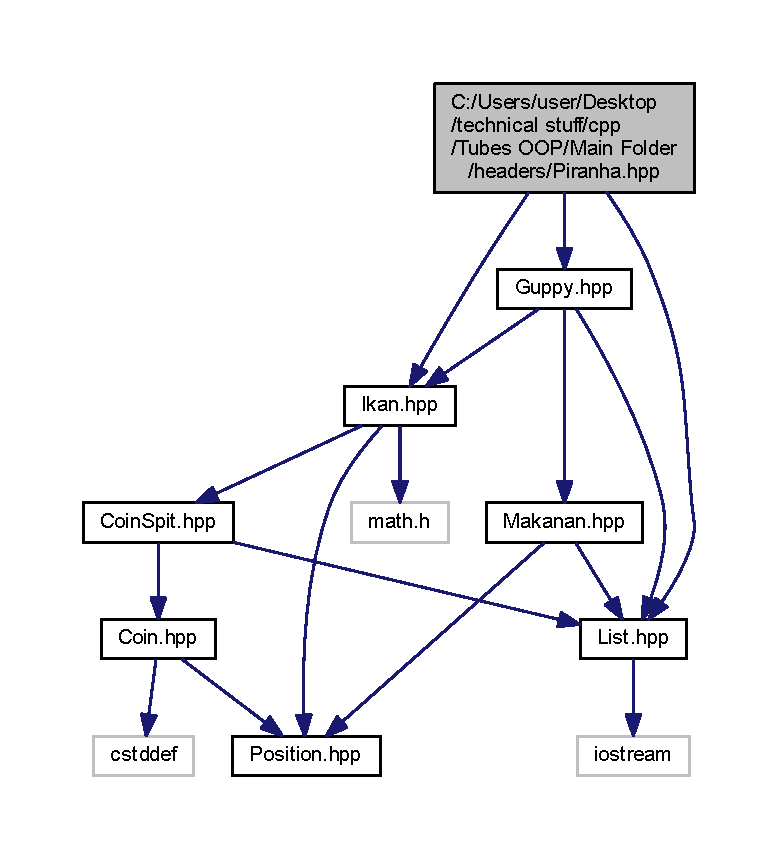
\includegraphics[width=350pt]{_piranha_8hpp__incl}
\end{center}
\end{figure}
This graph shows which files directly or indirectly include this file\+:
\nopagebreak
\begin{figure}[H]
\begin{center}
\leavevmode
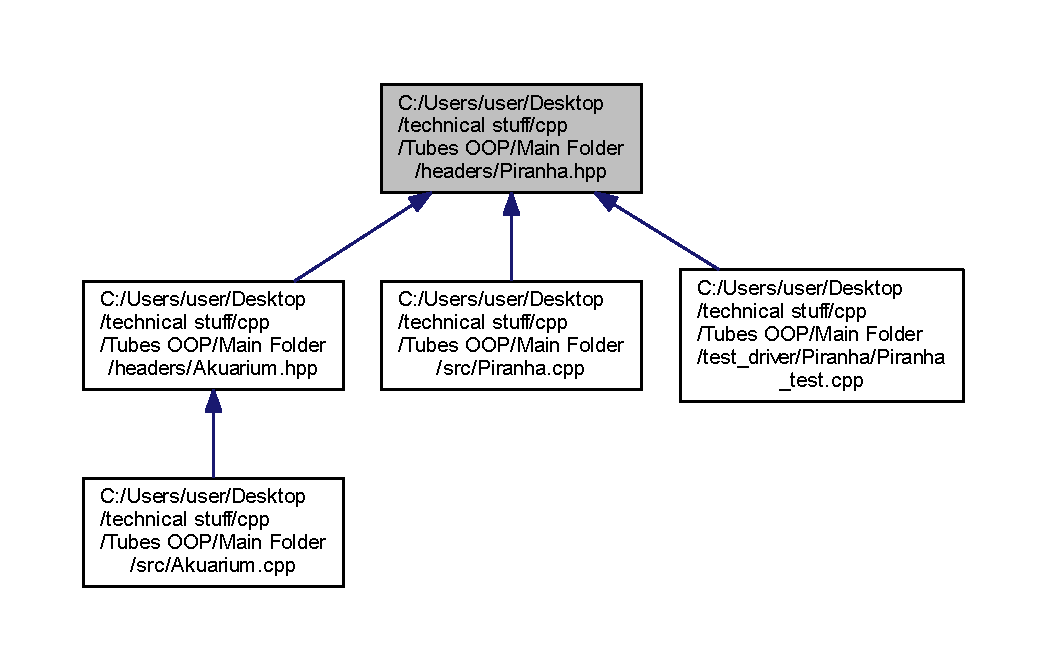
\includegraphics[width=350pt]{_piranha_8hpp__dep__incl}
\end{center}
\end{figure}
\subsection*{Classes}
\begin{DoxyCompactItemize}
\item 
class \mbox{\hyperlink{class_piranha}{Piranha}}
\end{DoxyCompactItemize}

\hypertarget{_position_8hpp}{}\section{headers/\+Position.hpp File Reference}
\label{_position_8hpp}\index{headers/\+Position.\+hpp@{headers/\+Position.\+hpp}}
This graph shows which files directly or indirectly include this file\+:
\nopagebreak
\begin{figure}[H]
\begin{center}
\leavevmode
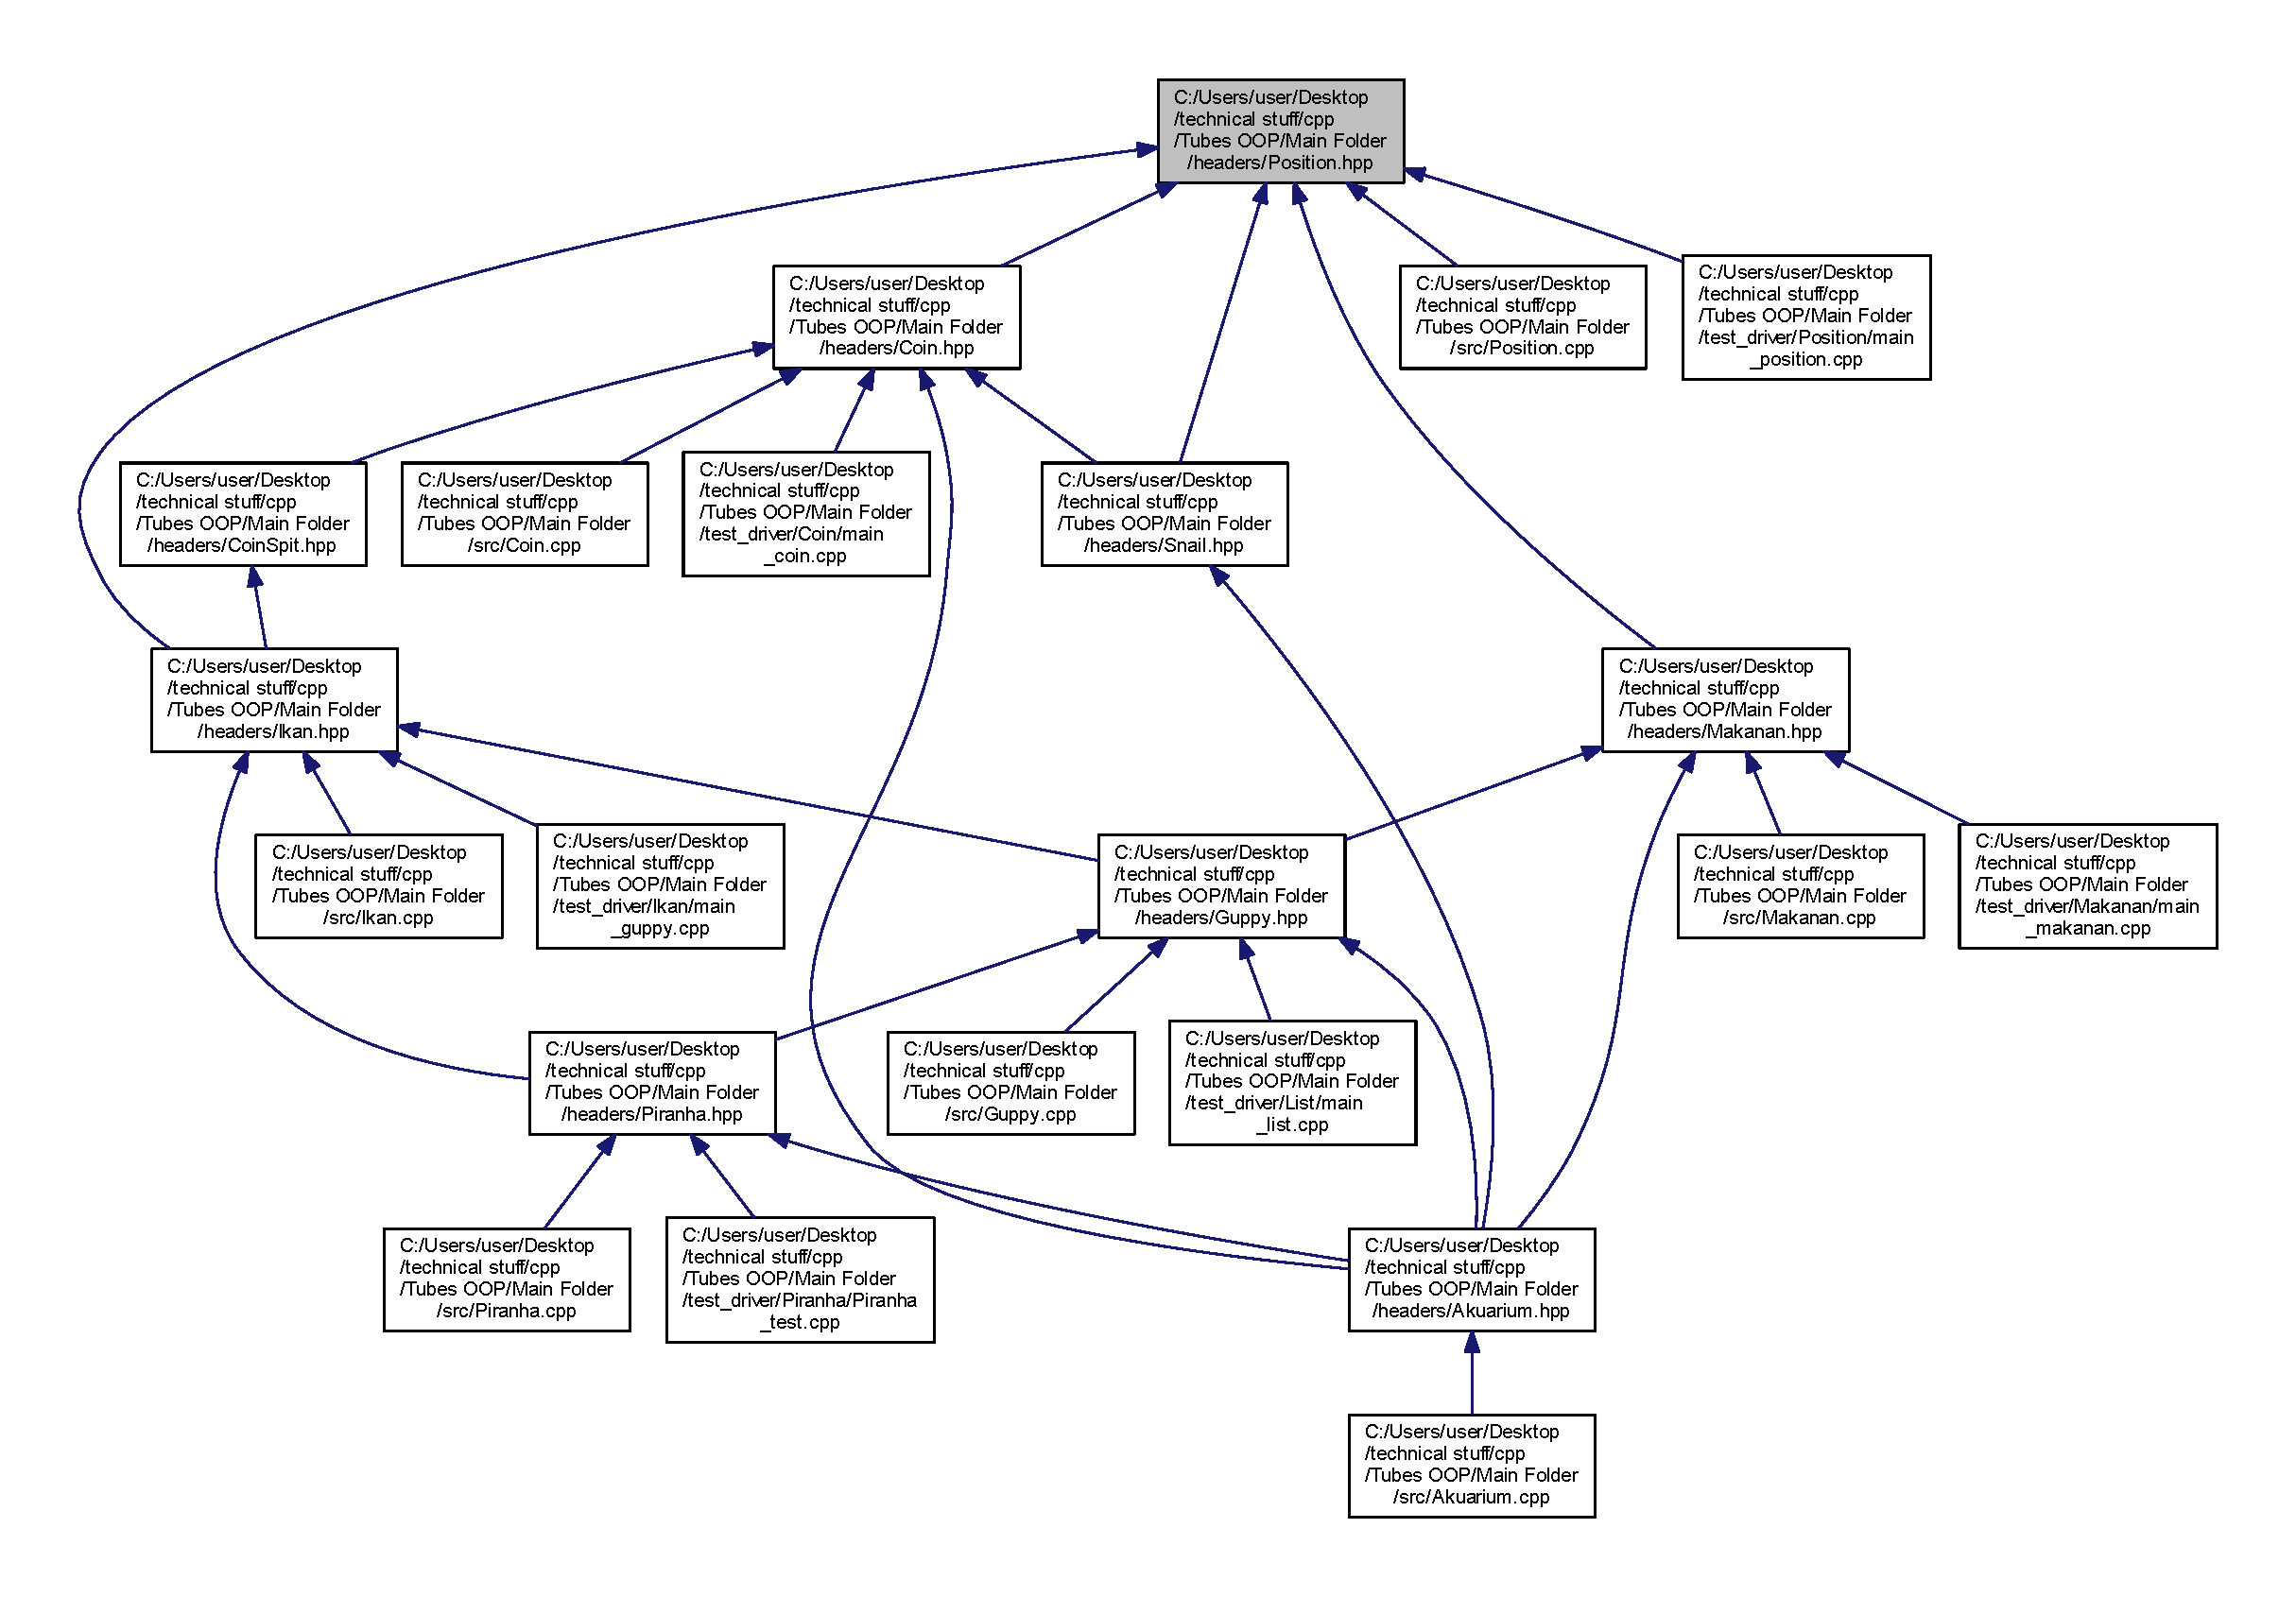
\includegraphics[width=350pt]{_position_8hpp__dep__incl}
\end{center}
\end{figure}
\subsection*{Classes}
\begin{DoxyCompactItemize}
\item 
class \mbox{\hyperlink{class_position}{Position}}
\end{DoxyCompactItemize}

\hypertarget{_snail_8hpp}{}\section{headers/\+Snail.hpp File Reference}
\label{_snail_8hpp}\index{headers/\+Snail.\+hpp@{headers/\+Snail.\+hpp}}
{\ttfamily \#include \char`\"{}Position.\+hpp\char`\"{}}\newline
{\ttfamily \#include \char`\"{}Coin.\+hpp\char`\"{}}\newline
{\ttfamily \#include \char`\"{}List.\+hpp\char`\"{}}\newline
Include dependency graph for Snail.\+hpp\+:
\nopagebreak
\begin{figure}[H]
\begin{center}
\leavevmode
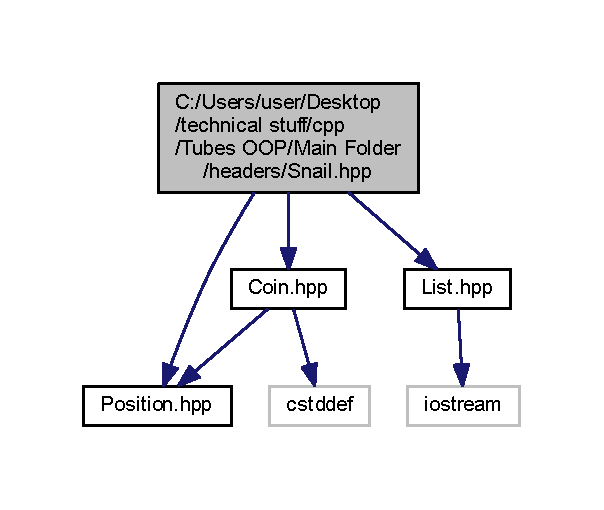
\includegraphics[width=290pt]{_snail_8hpp__incl}
\end{center}
\end{figure}
This graph shows which files directly or indirectly include this file\+:
\nopagebreak
\begin{figure}[H]
\begin{center}
\leavevmode
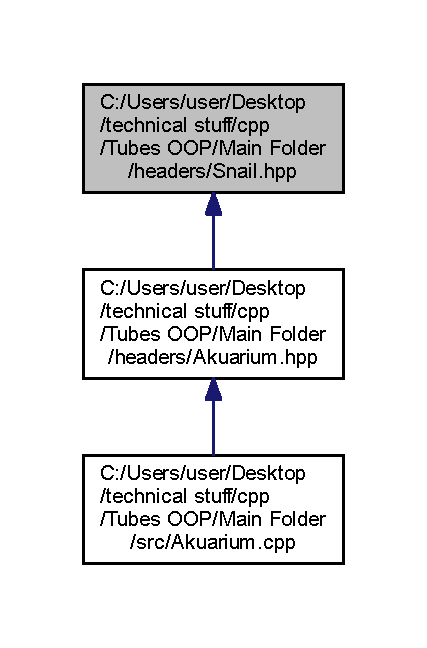
\includegraphics[width=303pt]{_snail_8hpp__dep__incl}
\end{center}
\end{figure}
\subsection*{Classes}
\begin{DoxyCompactItemize}
\item 
class \mbox{\hyperlink{class_snail}{Snail}}
\end{DoxyCompactItemize}

\hypertarget{main_8cpp}{}\section{main.\+cpp File Reference}
\label{main_8cpp}\index{main.\+cpp@{main.\+cpp}}
{\ttfamily \#include \char`\"{}oop.\+hpp\char`\"{}}\newline
{\ttfamily \#include \char`\"{}Akuarium.\+hpp\char`\"{}}\newline
{\ttfamily \#include $<$iostream$>$}\newline
{\ttfamily \#include $<$math.\+h$>$}\newline
{\ttfamily \#include $<$sstream$>$}\newline
{\ttfamily \#include $<$stdio.\+h$>$}\newline
Include dependency graph for main.\+cpp\+:
\nopagebreak
\begin{figure}[H]
\begin{center}
\leavevmode
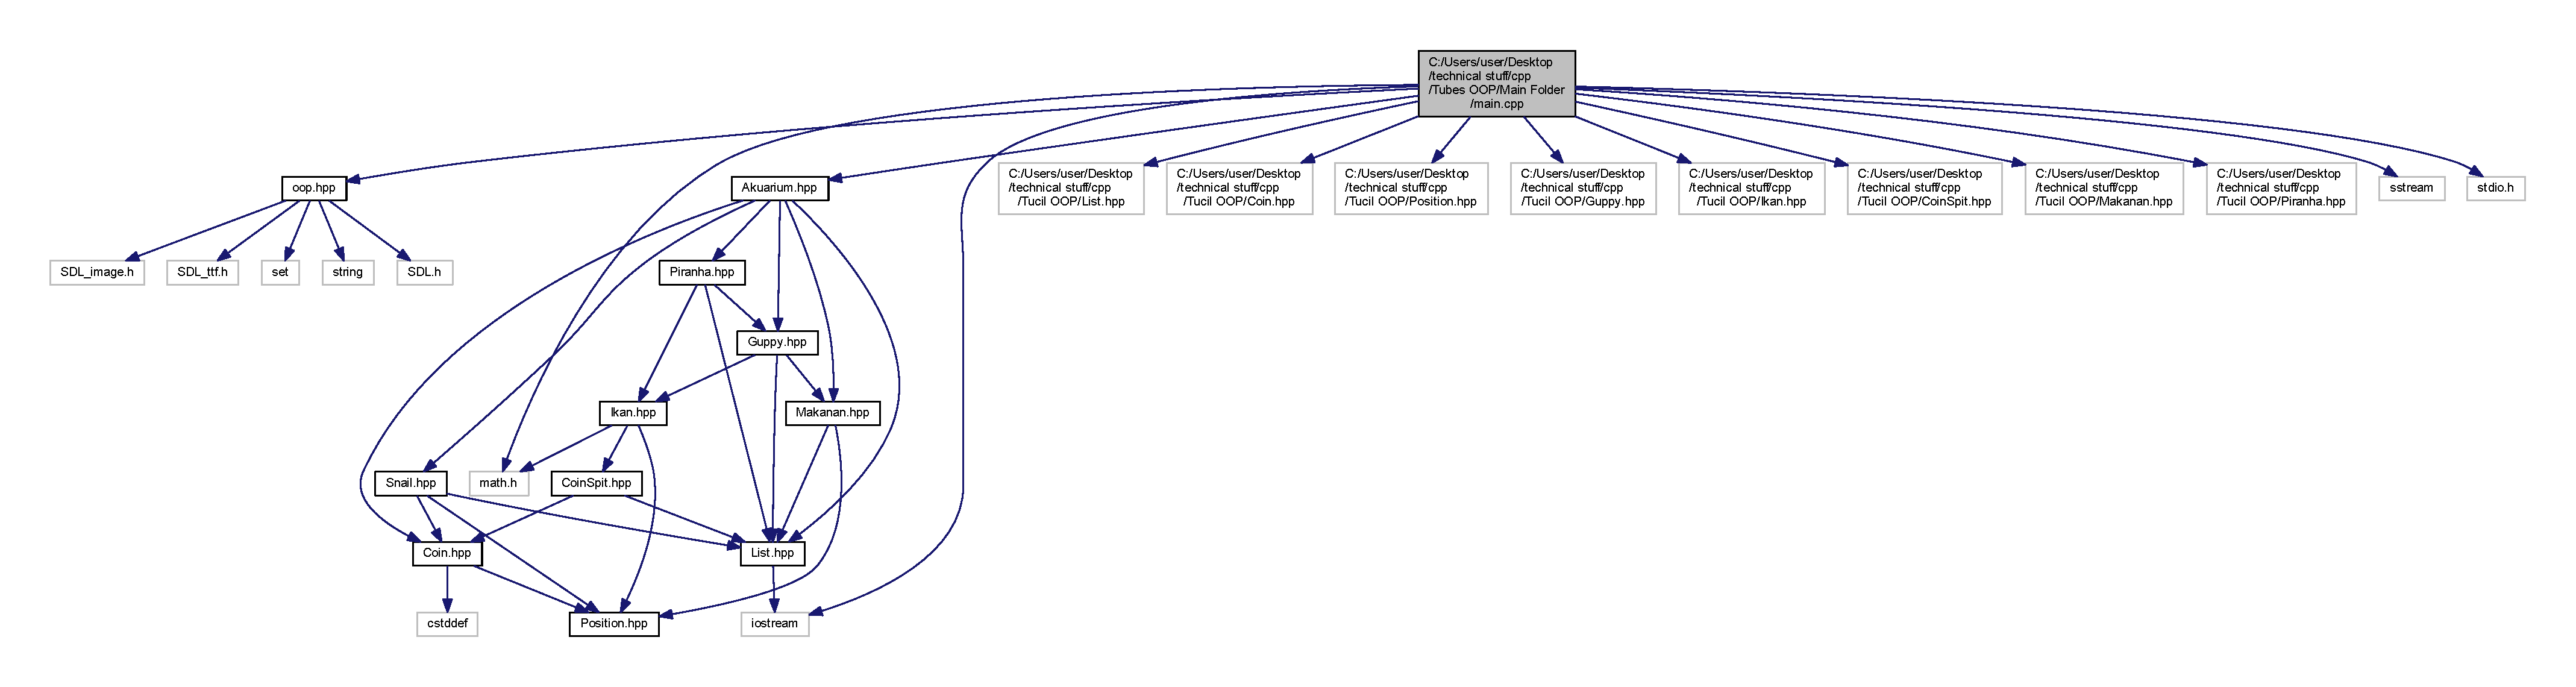
\includegraphics[width=350pt]{main_8cpp__incl}
\end{center}
\end{figure}
\subsection*{Functions}
\begin{DoxyCompactItemize}
\item 
int \mbox{\hyperlink{main_8cpp_a700a0caa5b70a06d1064e576f9f3cf65}{main}} (int argc, char $\ast$args\mbox{[}$\,$\mbox{]})
\end{DoxyCompactItemize}
\subsection*{Variables}
\begin{DoxyCompactItemize}
\item 
const double \mbox{\hyperlink{main_8cpp_a71fd37308050cd439537c5c6c2cb4614}{speed}} = 50
\end{DoxyCompactItemize}


\subsection{Function Documentation}
\mbox{\Hypertarget{main_8cpp_a700a0caa5b70a06d1064e576f9f3cf65}\label{main_8cpp_a700a0caa5b70a06d1064e576f9f3cf65}} 
\index{main.\+cpp@{main.\+cpp}!main@{main}}
\index{main@{main}!main.\+cpp@{main.\+cpp}}
\subsubsection{\texorpdfstring{main()}{main()}}
{\footnotesize\ttfamily int main (\begin{DoxyParamCaption}\item[{int}]{argc,  }\item[{char $\ast$}]{args\mbox{[}$\,$\mbox{]} }\end{DoxyParamCaption})}



\subsection{Variable Documentation}
\mbox{\Hypertarget{main_8cpp_a71fd37308050cd439537c5c6c2cb4614}\label{main_8cpp_a71fd37308050cd439537c5c6c2cb4614}} 
\index{main.\+cpp@{main.\+cpp}!speed@{speed}}
\index{speed@{speed}!main.\+cpp@{main.\+cpp}}
\subsubsection{\texorpdfstring{speed}{speed}}
{\footnotesize\ttfamily const double speed = 50}


\hypertarget{_akuarium_8cpp}{}\section{src/\+Akuarium.cpp File Reference}
\label{_akuarium_8cpp}\index{src/\+Akuarium.\+cpp@{src/\+Akuarium.\+cpp}}
{\ttfamily \#include \char`\"{}Akuarium.\+hpp\char`\"{}}\newline
{\ttfamily \#include $<$stdlib.\+h$>$}\newline
{\ttfamily \#include $<$time.\+h$>$}\newline
Include dependency graph for Akuarium.\+cpp\+:
\nopagebreak
\begin{figure}[H]
\begin{center}
\leavevmode
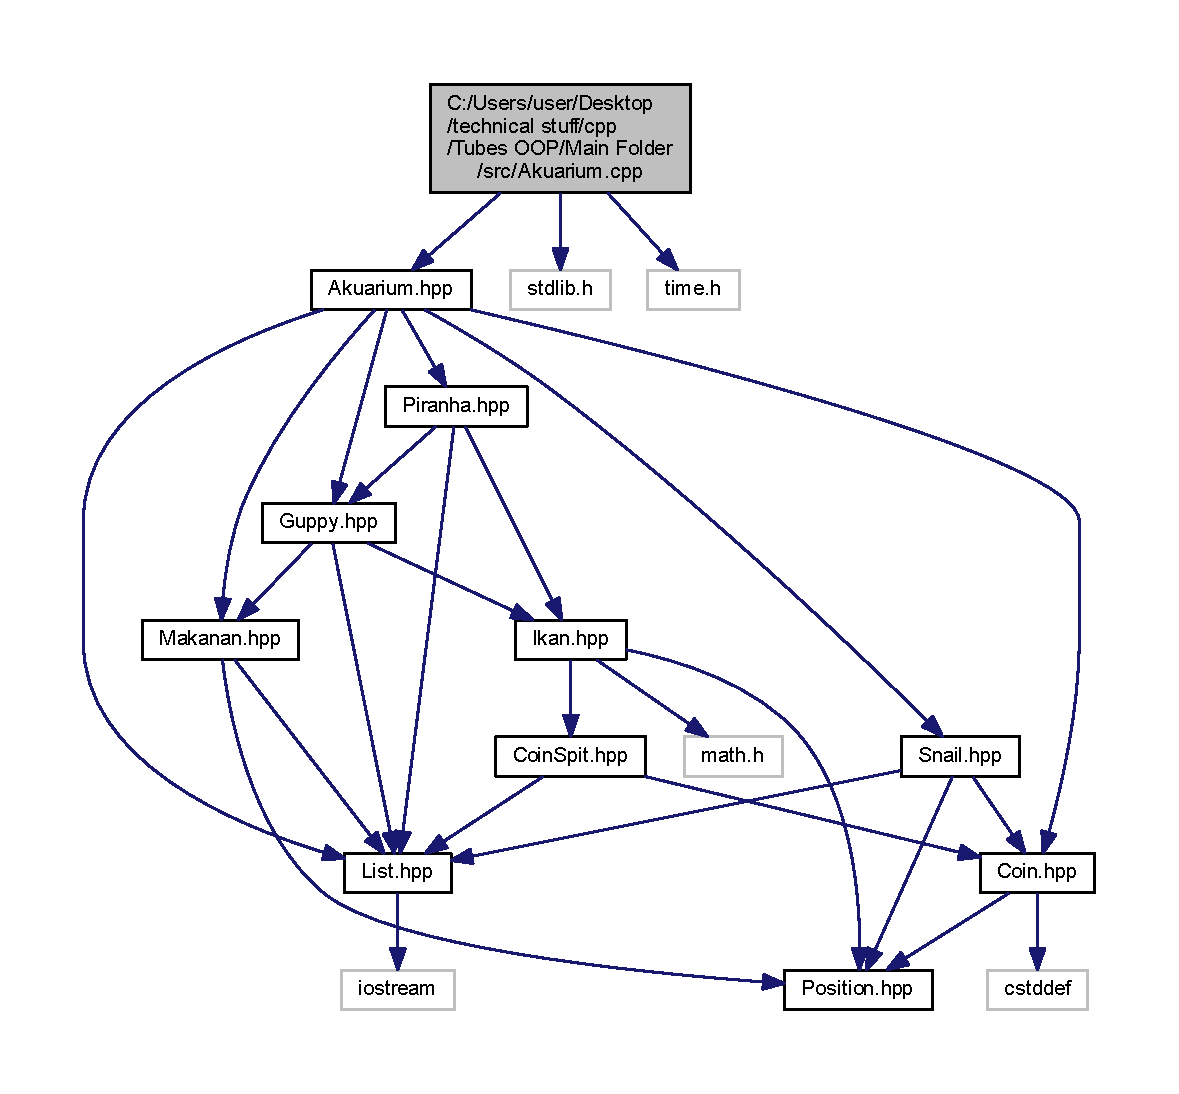
\includegraphics[width=350pt]{_akuarium_8cpp__incl}
\end{center}
\end{figure}

\hypertarget{_coin_8cpp}{}\section{src/\+Coin.cpp File Reference}
\label{_coin_8cpp}\index{src/\+Coin.\+cpp@{src/\+Coin.\+cpp}}
{\ttfamily \#include \char`\"{}Coin.\+hpp\char`\"{}}\newline
{\ttfamily \#include $<$stdlib.\+h$>$}\newline
Include dependency graph for Coin.\+cpp\+:
\nopagebreak
\begin{figure}[H]
\begin{center}
\leavevmode
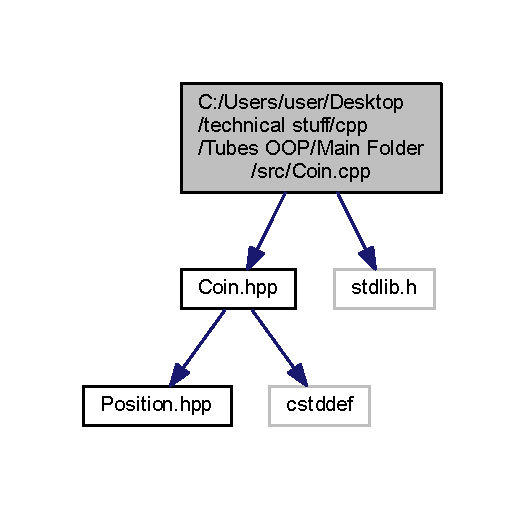
\includegraphics[width=249pt]{_coin_8cpp__incl}
\end{center}
\end{figure}

\hypertarget{_guppy_8cpp}{}\section{C\+:/\+Users/user/\+Desktop/technical stuff/cpp/\+Tubes O\+O\+P/\+Main Folder/src/\+Guppy.cpp File Reference}
\label{_guppy_8cpp}\index{C\+:/\+Users/user/\+Desktop/technical stuff/cpp/\+Tubes O\+O\+P/\+Main Folder/src/\+Guppy.\+cpp@{C\+:/\+Users/user/\+Desktop/technical stuff/cpp/\+Tubes O\+O\+P/\+Main Folder/src/\+Guppy.\+cpp}}
{\ttfamily \#include \char`\"{}Guppy.\+hpp\char`\"{}}\newline
{\ttfamily \#include $<$stdlib.\+h$>$}\newline
{\ttfamily \#include $<$time.\+h$>$}\newline
{\ttfamily \#include $<$stdio.\+h$>$}\newline
Include dependency graph for Guppy.\+cpp\+:
\nopagebreak
\begin{figure}[H]
\begin{center}
\leavevmode
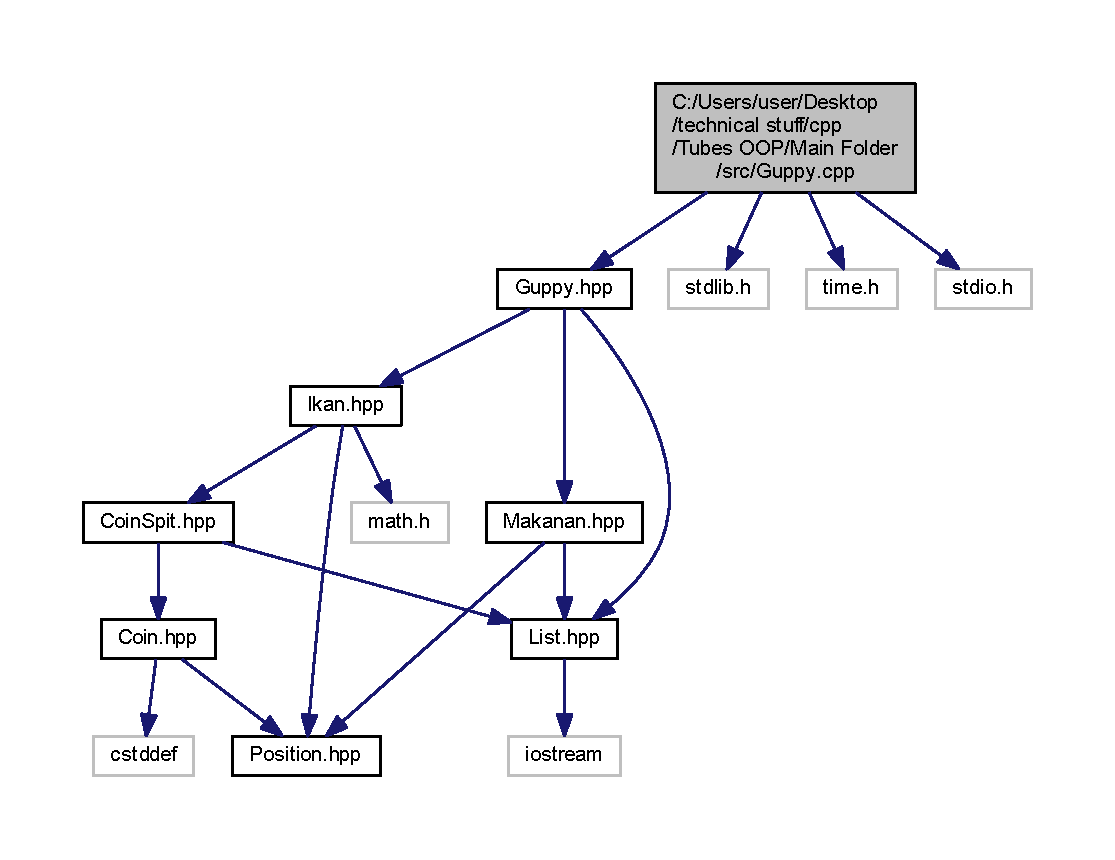
\includegraphics[width=350pt]{_guppy_8cpp__incl}
\end{center}
\end{figure}

\hypertarget{_ikan_8cpp}{}\section{src/\+Ikan.cpp File Reference}
\label{_ikan_8cpp}\index{src/\+Ikan.\+cpp@{src/\+Ikan.\+cpp}}
{\ttfamily \#include \char`\"{}Ikan.\+hpp\char`\"{}}\newline
{\ttfamily \#include \char`\"{}oop.\+hpp\char`\"{}}\newline
{\ttfamily \#include $<$stdio.\+h$>$}\newline
{\ttfamily \#include $<$time.\+h$>$}\newline
Include dependency graph for Ikan.\+cpp\+:
\nopagebreak
\begin{figure}[H]
\begin{center}
\leavevmode
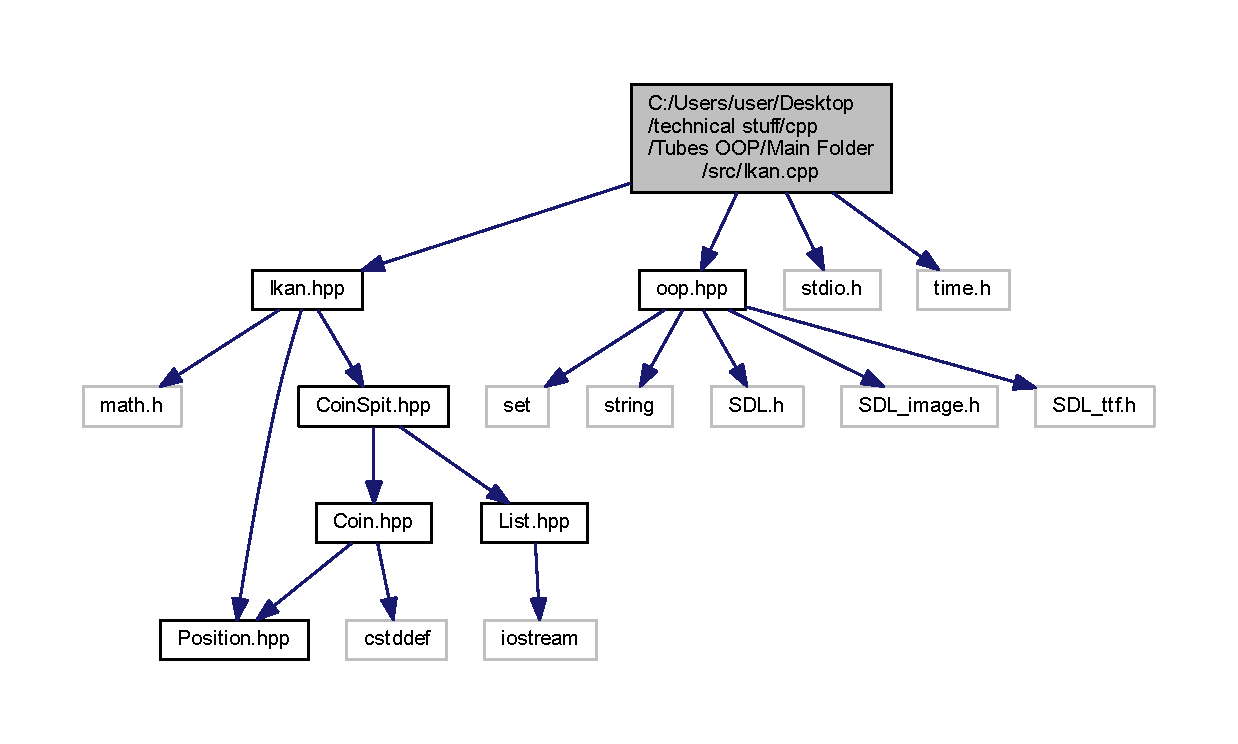
\includegraphics[width=350pt]{_ikan_8cpp__incl}
\end{center}
\end{figure}

\hypertarget{_makanan_8cpp}{}\section{src/\+Makanan.cpp File Reference}
\label{_makanan_8cpp}\index{src/\+Makanan.\+cpp@{src/\+Makanan.\+cpp}}
{\ttfamily \#include \char`\"{}Makanan.\+hpp\char`\"{}}\newline
Include dependency graph for Makanan.\+cpp\+:
\nopagebreak
\begin{figure}[H]
\begin{center}
\leavevmode
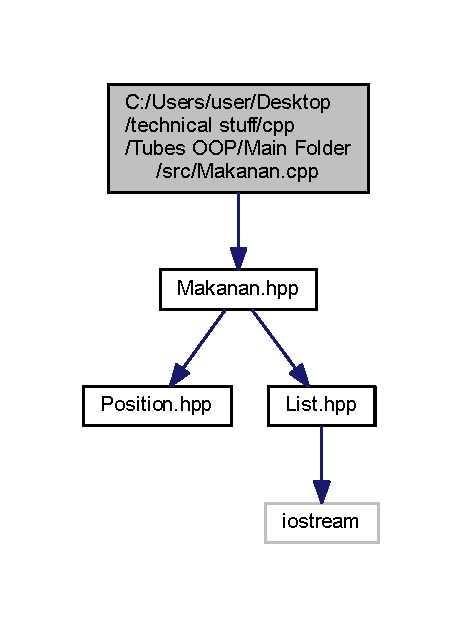
\includegraphics[width=222pt]{_makanan_8cpp__incl}
\end{center}
\end{figure}

\hypertarget{oop_8cpp}{}\section{C\+:/\+Users/user/\+Desktop/technical stuff/cpp/\+Tubes O\+O\+P/\+Main Folder/src/oop.cpp File Reference}
\label{oop_8cpp}\index{C\+:/\+Users/user/\+Desktop/technical stuff/cpp/\+Tubes O\+O\+P/\+Main Folder/src/oop.\+cpp@{C\+:/\+Users/user/\+Desktop/technical stuff/cpp/\+Tubes O\+O\+P/\+Main Folder/src/oop.\+cpp}}
{\ttfamily \#include \char`\"{}oop.\+hpp\char`\"{}}\newline
{\ttfamily \#include $<$map$>$}\newline
{\ttfamily \#include $<$iostream$>$}\newline
{\ttfamily \#include $<$chrono$>$}\newline
Include dependency graph for oop.\+cpp\+:
\nopagebreak
\begin{figure}[H]
\begin{center}
\leavevmode
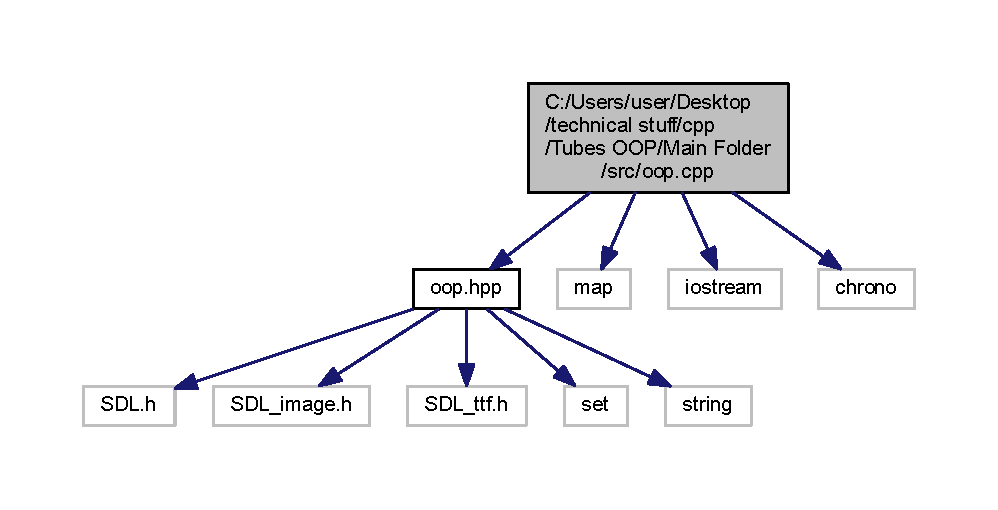
\includegraphics[width=350pt]{oop_8cpp__incl}
\end{center}
\end{figure}
\subsection*{Functions}
\begin{DoxyCompactItemize}
\item 
double \mbox{\hyperlink{oop_8cpp_a1ba1773fee3381786a816dc207a1f8d5}{time\+\_\+since\+\_\+start}} ()
\item 
bool \mbox{\hyperlink{oop_8cpp_aee8048628ff2b5c026c9e15acdcaacb8}{init}} ()
\item 
void \mbox{\hyperlink{oop_8cpp_a5ae591df94fc66ccb85cbb6565368bca}{close}} ()
\item 
S\+D\+L\+\_\+\+Surface $\ast$ \mbox{\hyperlink{oop_8cpp_a0e7ac416d5997995bce4c268daa46686}{load\+Surface}} (std\+::string path)
\item 
void \mbox{\hyperlink{oop_8cpp_a0f01596e4fd0a81c514c706c4936ee8d}{draw\+\_\+image}} (std\+::string filename, int x, int y)
\item 
void \mbox{\hyperlink{oop_8cpp_a2b13ce610f0fb0df7a95eb2307e319d2}{draw\+\_\+text}} (std\+::string text, int font\+\_\+size, int x, int y, unsigned char r, unsigned char g, unsigned char b)
\item 
void \mbox{\hyperlink{oop_8cpp_a4953d1edcbbfc7e420c423ded1d5621a}{clear\+\_\+screen}} ()
\item 
void \mbox{\hyperlink{oop_8cpp_a10da25e92e69613be93d099bb029feb2}{update\+\_\+screen}} ()
\item 
void \mbox{\hyperlink{oop_8cpp_ab19fbad269feb4f8cf725031233ba56e}{handle\+\_\+input}} ()
\item 
bool \mbox{\hyperlink{oop_8cpp_a1b14e3b0f5799f93f8dab7f5c6819298}{quit\+\_\+pressed}} ()
\item 
const std\+::set$<$ S\+D\+L\+\_\+\+Keycode $>$ \& \mbox{\hyperlink{oop_8cpp_a155dba9d2b234776d0fb743da0dcdbc2}{get\+\_\+pressed\+\_\+keys}} ()
\item 
const std\+::set$<$ S\+D\+L\+\_\+\+Keycode $>$ \& \mbox{\hyperlink{oop_8cpp_a4fdfe498ed93ea27801b69f2158e5e6a}{get\+\_\+tapped\+\_\+keys}} ()
\item 
const std\+::set$<$ Uint8 $>$ \& \mbox{\hyperlink{oop_8cpp_a921d1df60af4bfb75d55de50bf6d1e19}{get\+\_\+pressed\+\_\+buttons}} ()
\item 
const std\+::set$<$ Uint8 $>$ \& \mbox{\hyperlink{oop_8cpp_abe85482fb212faff74cb7e33060d2f1d}{get\+\_\+tapped\+\_\+buttons}} ()
\end{DoxyCompactItemize}
\subsection*{Variables}
\begin{DoxyCompactItemize}
\item 
high\+\_\+resolution\+\_\+clock\+::time\+\_\+point \mbox{\hyperlink{oop_8cpp_a1735b8c468a759db2a102e031c6b1436}{start}} = high\+\_\+resolution\+\_\+clock\+::now()
\item 
S\+D\+L\+\_\+\+Window $\ast$ \mbox{\hyperlink{oop_8cpp_a7d570c1c3b1ac98019869517e6062462}{sdl\+Window}}
\item 
std\+::map$<$ std\+::string, S\+D\+L\+\_\+\+Surface $\ast$ $>$ \mbox{\hyperlink{oop_8cpp_a628cbb50ed852f954df9e6e5288b9f1c}{loaded\+Surfaces}}
\item 
std\+::map$<$ int, T\+T\+F\+\_\+\+Font $\ast$ $>$ \mbox{\hyperlink{oop_8cpp_a3dd6e6fa4b946f1a7c7325b7be30835e}{loaded\+Font\+Sizes}}
\item 
S\+D\+L\+\_\+\+Surface $\ast$ \mbox{\hyperlink{oop_8cpp_aa93b1188c9e7061fda6ed6d81cd1a774}{g\+Screen\+Surface}} = N\+U\+LL
\item 
bool \mbox{\hyperlink{oop_8cpp_ac746fa6ad48d19984a159f14bec028a3}{quit}} = false
\item 
std\+::set$<$ S\+D\+L\+\_\+\+Keycode $>$ \mbox{\hyperlink{oop_8cpp_a82122c0a11768870334b09ab6483f96c}{pressed\+Keys}}
\item 
std\+::set$<$ S\+D\+L\+\_\+\+Keycode $>$ \mbox{\hyperlink{oop_8cpp_afee38be0153d2eb7d46f4f1fd9d3dc8b}{tapped\+Keys}}
\item 
std\+::set$<$ Uint8 $>$ \mbox{\hyperlink{oop_8cpp_ade21f229589b6bfbf3184ce8d5aa6d32}{pressed\+Button}}
\item 
std\+::set$<$ Uint8 $>$ \mbox{\hyperlink{oop_8cpp_a715eac185b6e88c0dad3d79f28882b9c}{tapped\+Button}}
\end{DoxyCompactItemize}


\subsection{Function Documentation}
\mbox{\Hypertarget{oop_8cpp_a4953d1edcbbfc7e420c423ded1d5621a}\label{oop_8cpp_a4953d1edcbbfc7e420c423ded1d5621a}} 
\index{oop.\+cpp@{oop.\+cpp}!clear\+\_\+screen@{clear\+\_\+screen}}
\index{clear\+\_\+screen@{clear\+\_\+screen}!oop.\+cpp@{oop.\+cpp}}
\subsubsection{\texorpdfstring{clear\+\_\+screen()}{clear\_screen()}}
{\footnotesize\ttfamily void clear\+\_\+screen (\begin{DoxyParamCaption}{ }\end{DoxyParamCaption})}

\mbox{\Hypertarget{oop_8cpp_a5ae591df94fc66ccb85cbb6565368bca}\label{oop_8cpp_a5ae591df94fc66ccb85cbb6565368bca}} 
\index{oop.\+cpp@{oop.\+cpp}!close@{close}}
\index{close@{close}!oop.\+cpp@{oop.\+cpp}}
\subsubsection{\texorpdfstring{close()}{close()}}
{\footnotesize\ttfamily void close (\begin{DoxyParamCaption}{ }\end{DoxyParamCaption})}

\mbox{\Hypertarget{oop_8cpp_a0f01596e4fd0a81c514c706c4936ee8d}\label{oop_8cpp_a0f01596e4fd0a81c514c706c4936ee8d}} 
\index{oop.\+cpp@{oop.\+cpp}!draw\+\_\+image@{draw\+\_\+image}}
\index{draw\+\_\+image@{draw\+\_\+image}!oop.\+cpp@{oop.\+cpp}}
\subsubsection{\texorpdfstring{draw\+\_\+image()}{draw\_image()}}
{\footnotesize\ttfamily void draw\+\_\+image (\begin{DoxyParamCaption}\item[{std\+::string}]{filename,  }\item[{int}]{x,  }\item[{int}]{y }\end{DoxyParamCaption})}

\mbox{\Hypertarget{oop_8cpp_a2b13ce610f0fb0df7a95eb2307e319d2}\label{oop_8cpp_a2b13ce610f0fb0df7a95eb2307e319d2}} 
\index{oop.\+cpp@{oop.\+cpp}!draw\+\_\+text@{draw\+\_\+text}}
\index{draw\+\_\+text@{draw\+\_\+text}!oop.\+cpp@{oop.\+cpp}}
\subsubsection{\texorpdfstring{draw\+\_\+text()}{draw\_text()}}
{\footnotesize\ttfamily void draw\+\_\+text (\begin{DoxyParamCaption}\item[{std\+::string}]{text,  }\item[{int}]{font\+\_\+size,  }\item[{int}]{x,  }\item[{int}]{y,  }\item[{unsigned char}]{r,  }\item[{unsigned char}]{g,  }\item[{unsigned char}]{b }\end{DoxyParamCaption})}

\mbox{\Hypertarget{oop_8cpp_a921d1df60af4bfb75d55de50bf6d1e19}\label{oop_8cpp_a921d1df60af4bfb75d55de50bf6d1e19}} 
\index{oop.\+cpp@{oop.\+cpp}!get\+\_\+pressed\+\_\+buttons@{get\+\_\+pressed\+\_\+buttons}}
\index{get\+\_\+pressed\+\_\+buttons@{get\+\_\+pressed\+\_\+buttons}!oop.\+cpp@{oop.\+cpp}}
\subsubsection{\texorpdfstring{get\+\_\+pressed\+\_\+buttons()}{get\_pressed\_buttons()}}
{\footnotesize\ttfamily const std\+::set$<$Uint8$>$\& get\+\_\+pressed\+\_\+buttons (\begin{DoxyParamCaption}{ }\end{DoxyParamCaption})}

\mbox{\Hypertarget{oop_8cpp_a155dba9d2b234776d0fb743da0dcdbc2}\label{oop_8cpp_a155dba9d2b234776d0fb743da0dcdbc2}} 
\index{oop.\+cpp@{oop.\+cpp}!get\+\_\+pressed\+\_\+keys@{get\+\_\+pressed\+\_\+keys}}
\index{get\+\_\+pressed\+\_\+keys@{get\+\_\+pressed\+\_\+keys}!oop.\+cpp@{oop.\+cpp}}
\subsubsection{\texorpdfstring{get\+\_\+pressed\+\_\+keys()}{get\_pressed\_keys()}}
{\footnotesize\ttfamily const std\+::set$<$S\+D\+L\+\_\+\+Keycode$>$\& get\+\_\+pressed\+\_\+keys (\begin{DoxyParamCaption}{ }\end{DoxyParamCaption})}

\mbox{\Hypertarget{oop_8cpp_abe85482fb212faff74cb7e33060d2f1d}\label{oop_8cpp_abe85482fb212faff74cb7e33060d2f1d}} 
\index{oop.\+cpp@{oop.\+cpp}!get\+\_\+tapped\+\_\+buttons@{get\+\_\+tapped\+\_\+buttons}}
\index{get\+\_\+tapped\+\_\+buttons@{get\+\_\+tapped\+\_\+buttons}!oop.\+cpp@{oop.\+cpp}}
\subsubsection{\texorpdfstring{get\+\_\+tapped\+\_\+buttons()}{get\_tapped\_buttons()}}
{\footnotesize\ttfamily const std\+::set$<$Uint8$>$\& get\+\_\+tapped\+\_\+buttons (\begin{DoxyParamCaption}{ }\end{DoxyParamCaption})}

\mbox{\Hypertarget{oop_8cpp_a4fdfe498ed93ea27801b69f2158e5e6a}\label{oop_8cpp_a4fdfe498ed93ea27801b69f2158e5e6a}} 
\index{oop.\+cpp@{oop.\+cpp}!get\+\_\+tapped\+\_\+keys@{get\+\_\+tapped\+\_\+keys}}
\index{get\+\_\+tapped\+\_\+keys@{get\+\_\+tapped\+\_\+keys}!oop.\+cpp@{oop.\+cpp}}
\subsubsection{\texorpdfstring{get\+\_\+tapped\+\_\+keys()}{get\_tapped\_keys()}}
{\footnotesize\ttfamily const std\+::set$<$S\+D\+L\+\_\+\+Keycode$>$\& get\+\_\+tapped\+\_\+keys (\begin{DoxyParamCaption}{ }\end{DoxyParamCaption})}

\mbox{\Hypertarget{oop_8cpp_ab19fbad269feb4f8cf725031233ba56e}\label{oop_8cpp_ab19fbad269feb4f8cf725031233ba56e}} 
\index{oop.\+cpp@{oop.\+cpp}!handle\+\_\+input@{handle\+\_\+input}}
\index{handle\+\_\+input@{handle\+\_\+input}!oop.\+cpp@{oop.\+cpp}}
\subsubsection{\texorpdfstring{handle\+\_\+input()}{handle\_input()}}
{\footnotesize\ttfamily void handle\+\_\+input (\begin{DoxyParamCaption}{ }\end{DoxyParamCaption})}

\mbox{\Hypertarget{oop_8cpp_aee8048628ff2b5c026c9e15acdcaacb8}\label{oop_8cpp_aee8048628ff2b5c026c9e15acdcaacb8}} 
\index{oop.\+cpp@{oop.\+cpp}!init@{init}}
\index{init@{init}!oop.\+cpp@{oop.\+cpp}}
\subsubsection{\texorpdfstring{init()}{init()}}
{\footnotesize\ttfamily bool init (\begin{DoxyParamCaption}{ }\end{DoxyParamCaption})}

\mbox{\Hypertarget{oop_8cpp_a0e7ac416d5997995bce4c268daa46686}\label{oop_8cpp_a0e7ac416d5997995bce4c268daa46686}} 
\index{oop.\+cpp@{oop.\+cpp}!load\+Surface@{load\+Surface}}
\index{load\+Surface@{load\+Surface}!oop.\+cpp@{oop.\+cpp}}
\subsubsection{\texorpdfstring{load\+Surface()}{loadSurface()}}
{\footnotesize\ttfamily S\+D\+L\+\_\+\+Surface$\ast$ load\+Surface (\begin{DoxyParamCaption}\item[{std\+::string}]{path }\end{DoxyParamCaption})}

\mbox{\Hypertarget{oop_8cpp_a1b14e3b0f5799f93f8dab7f5c6819298}\label{oop_8cpp_a1b14e3b0f5799f93f8dab7f5c6819298}} 
\index{oop.\+cpp@{oop.\+cpp}!quit\+\_\+pressed@{quit\+\_\+pressed}}
\index{quit\+\_\+pressed@{quit\+\_\+pressed}!oop.\+cpp@{oop.\+cpp}}
\subsubsection{\texorpdfstring{quit\+\_\+pressed()}{quit\_pressed()}}
{\footnotesize\ttfamily bool quit\+\_\+pressed (\begin{DoxyParamCaption}{ }\end{DoxyParamCaption})}

\mbox{\Hypertarget{oop_8cpp_a1ba1773fee3381786a816dc207a1f8d5}\label{oop_8cpp_a1ba1773fee3381786a816dc207a1f8d5}} 
\index{oop.\+cpp@{oop.\+cpp}!time\+\_\+since\+\_\+start@{time\+\_\+since\+\_\+start}}
\index{time\+\_\+since\+\_\+start@{time\+\_\+since\+\_\+start}!oop.\+cpp@{oop.\+cpp}}
\subsubsection{\texorpdfstring{time\+\_\+since\+\_\+start()}{time\_since\_start()}}
{\footnotesize\ttfamily double time\+\_\+since\+\_\+start (\begin{DoxyParamCaption}{ }\end{DoxyParamCaption})}

\mbox{\Hypertarget{oop_8cpp_a10da25e92e69613be93d099bb029feb2}\label{oop_8cpp_a10da25e92e69613be93d099bb029feb2}} 
\index{oop.\+cpp@{oop.\+cpp}!update\+\_\+screen@{update\+\_\+screen}}
\index{update\+\_\+screen@{update\+\_\+screen}!oop.\+cpp@{oop.\+cpp}}
\subsubsection{\texorpdfstring{update\+\_\+screen()}{update\_screen()}}
{\footnotesize\ttfamily void update\+\_\+screen (\begin{DoxyParamCaption}{ }\end{DoxyParamCaption})}



\subsection{Variable Documentation}
\mbox{\Hypertarget{oop_8cpp_aa93b1188c9e7061fda6ed6d81cd1a774}\label{oop_8cpp_aa93b1188c9e7061fda6ed6d81cd1a774}} 
\index{oop.\+cpp@{oop.\+cpp}!g\+Screen\+Surface@{g\+Screen\+Surface}}
\index{g\+Screen\+Surface@{g\+Screen\+Surface}!oop.\+cpp@{oop.\+cpp}}
\subsubsection{\texorpdfstring{g\+Screen\+Surface}{gScreenSurface}}
{\footnotesize\ttfamily S\+D\+L\+\_\+\+Surface$\ast$ g\+Screen\+Surface = N\+U\+LL}

\mbox{\Hypertarget{oop_8cpp_a3dd6e6fa4b946f1a7c7325b7be30835e}\label{oop_8cpp_a3dd6e6fa4b946f1a7c7325b7be30835e}} 
\index{oop.\+cpp@{oop.\+cpp}!loaded\+Font\+Sizes@{loaded\+Font\+Sizes}}
\index{loaded\+Font\+Sizes@{loaded\+Font\+Sizes}!oop.\+cpp@{oop.\+cpp}}
\subsubsection{\texorpdfstring{loaded\+Font\+Sizes}{loadedFontSizes}}
{\footnotesize\ttfamily std\+::map$<$int, T\+T\+F\+\_\+\+Font$\ast$$>$ loaded\+Font\+Sizes}

\mbox{\Hypertarget{oop_8cpp_a628cbb50ed852f954df9e6e5288b9f1c}\label{oop_8cpp_a628cbb50ed852f954df9e6e5288b9f1c}} 
\index{oop.\+cpp@{oop.\+cpp}!loaded\+Surfaces@{loaded\+Surfaces}}
\index{loaded\+Surfaces@{loaded\+Surfaces}!oop.\+cpp@{oop.\+cpp}}
\subsubsection{\texorpdfstring{loaded\+Surfaces}{loadedSurfaces}}
{\footnotesize\ttfamily std\+::map$<$std\+::string, S\+D\+L\+\_\+\+Surface$\ast$$>$ loaded\+Surfaces}

\mbox{\Hypertarget{oop_8cpp_ade21f229589b6bfbf3184ce8d5aa6d32}\label{oop_8cpp_ade21f229589b6bfbf3184ce8d5aa6d32}} 
\index{oop.\+cpp@{oop.\+cpp}!pressed\+Button@{pressed\+Button}}
\index{pressed\+Button@{pressed\+Button}!oop.\+cpp@{oop.\+cpp}}
\subsubsection{\texorpdfstring{pressed\+Button}{pressedButton}}
{\footnotesize\ttfamily std\+::set$<$Uint8$>$ pressed\+Button}

\mbox{\Hypertarget{oop_8cpp_a82122c0a11768870334b09ab6483f96c}\label{oop_8cpp_a82122c0a11768870334b09ab6483f96c}} 
\index{oop.\+cpp@{oop.\+cpp}!pressed\+Keys@{pressed\+Keys}}
\index{pressed\+Keys@{pressed\+Keys}!oop.\+cpp@{oop.\+cpp}}
\subsubsection{\texorpdfstring{pressed\+Keys}{pressedKeys}}
{\footnotesize\ttfamily std\+::set$<$S\+D\+L\+\_\+\+Keycode$>$ pressed\+Keys}

\mbox{\Hypertarget{oop_8cpp_ac746fa6ad48d19984a159f14bec028a3}\label{oop_8cpp_ac746fa6ad48d19984a159f14bec028a3}} 
\index{oop.\+cpp@{oop.\+cpp}!quit@{quit}}
\index{quit@{quit}!oop.\+cpp@{oop.\+cpp}}
\subsubsection{\texorpdfstring{quit}{quit}}
{\footnotesize\ttfamily bool quit = false}

\mbox{\Hypertarget{oop_8cpp_a7d570c1c3b1ac98019869517e6062462}\label{oop_8cpp_a7d570c1c3b1ac98019869517e6062462}} 
\index{oop.\+cpp@{oop.\+cpp}!sdl\+Window@{sdl\+Window}}
\index{sdl\+Window@{sdl\+Window}!oop.\+cpp@{oop.\+cpp}}
\subsubsection{\texorpdfstring{sdl\+Window}{sdlWindow}}
{\footnotesize\ttfamily S\+D\+L\+\_\+\+Window$\ast$ sdl\+Window}

\mbox{\Hypertarget{oop_8cpp_a1735b8c468a759db2a102e031c6b1436}\label{oop_8cpp_a1735b8c468a759db2a102e031c6b1436}} 
\index{oop.\+cpp@{oop.\+cpp}!start@{start}}
\index{start@{start}!oop.\+cpp@{oop.\+cpp}}
\subsubsection{\texorpdfstring{start}{start}}
{\footnotesize\ttfamily high\+\_\+resolution\+\_\+clock\+::time\+\_\+point start = high\+\_\+resolution\+\_\+clock\+::now()}

\mbox{\Hypertarget{oop_8cpp_a715eac185b6e88c0dad3d79f28882b9c}\label{oop_8cpp_a715eac185b6e88c0dad3d79f28882b9c}} 
\index{oop.\+cpp@{oop.\+cpp}!tapped\+Button@{tapped\+Button}}
\index{tapped\+Button@{tapped\+Button}!oop.\+cpp@{oop.\+cpp}}
\subsubsection{\texorpdfstring{tapped\+Button}{tappedButton}}
{\footnotesize\ttfamily std\+::set$<$Uint8$>$ tapped\+Button}

\mbox{\Hypertarget{oop_8cpp_afee38be0153d2eb7d46f4f1fd9d3dc8b}\label{oop_8cpp_afee38be0153d2eb7d46f4f1fd9d3dc8b}} 
\index{oop.\+cpp@{oop.\+cpp}!tapped\+Keys@{tapped\+Keys}}
\index{tapped\+Keys@{tapped\+Keys}!oop.\+cpp@{oop.\+cpp}}
\subsubsection{\texorpdfstring{tapped\+Keys}{tappedKeys}}
{\footnotesize\ttfamily std\+::set$<$S\+D\+L\+\_\+\+Keycode$>$ tapped\+Keys}


\hypertarget{_piranha_8cpp}{}\section{C\+:/\+Users/user/\+Desktop/technical stuff/cpp/\+Tubes O\+O\+P/\+Main Folder/src/\+Piranha.cpp File Reference}
\label{_piranha_8cpp}\index{C\+:/\+Users/user/\+Desktop/technical stuff/cpp/\+Tubes O\+O\+P/\+Main Folder/src/\+Piranha.\+cpp@{C\+:/\+Users/user/\+Desktop/technical stuff/cpp/\+Tubes O\+O\+P/\+Main Folder/src/\+Piranha.\+cpp}}
{\ttfamily \#include \char`\"{}Piranha.\+hpp\char`\"{}}\newline
{\ttfamily \#include $<$stdlib.\+h$>$}\newline
{\ttfamily \#include $<$time.\+h$>$}\newline
Include dependency graph for Piranha.\+cpp\+:
\nopagebreak
\begin{figure}[H]
\begin{center}
\leavevmode
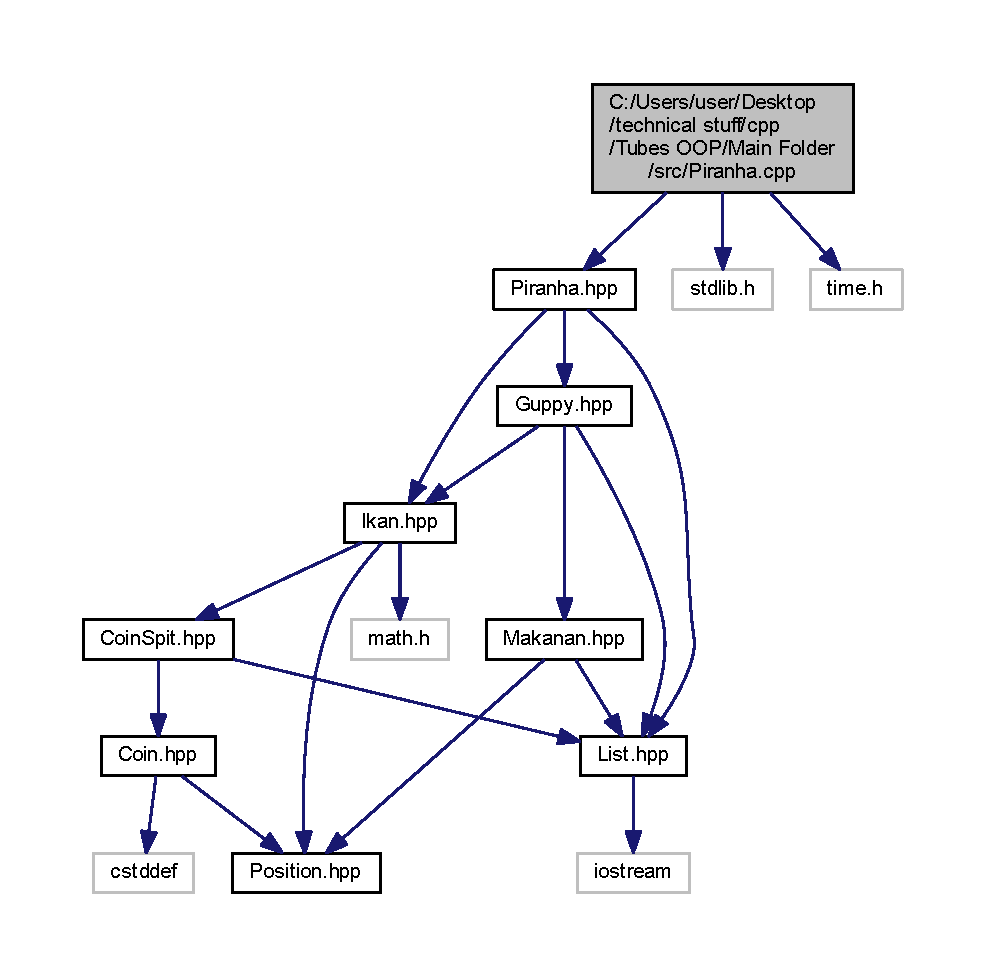
\includegraphics[width=350pt]{_piranha_8cpp__incl}
\end{center}
\end{figure}

\hypertarget{_position_8cpp}{}\section{src/\+Position.cpp File Reference}
\label{_position_8cpp}\index{src/\+Position.\+cpp@{src/\+Position.\+cpp}}
{\ttfamily \#include \char`\"{}Position.\+hpp\char`\"{}}\newline
{\ttfamily \#include $<$stdlib.\+h$>$}\newline
Include dependency graph for Position.\+cpp\+:
\nopagebreak
\begin{figure}[H]
\begin{center}
\leavevmode
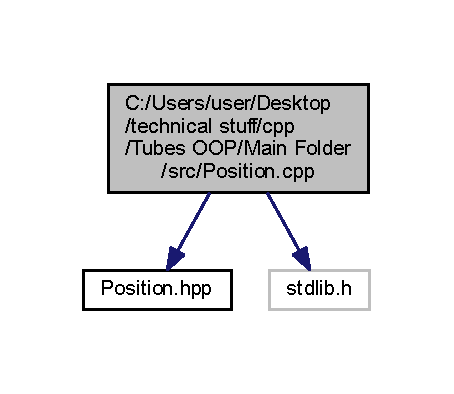
\includegraphics[width=218pt]{_position_8cpp__incl}
\end{center}
\end{figure}

\hypertarget{_snail_8cpp}{}\section{C\+:/\+Users/user/\+Desktop/technical stuff/cpp/\+Tubes O\+O\+P/\+Main Folder/src/\+Snail.cpp File Reference}
\label{_snail_8cpp}\index{C\+:/\+Users/user/\+Desktop/technical stuff/cpp/\+Tubes O\+O\+P/\+Main Folder/src/\+Snail.\+cpp@{C\+:/\+Users/user/\+Desktop/technical stuff/cpp/\+Tubes O\+O\+P/\+Main Folder/src/\+Snail.\+cpp}}
{\ttfamily \#include \char`\"{}Snail.\+hpp\char`\"{}}\newline
{\ttfamily \#include $<$math.\+h$>$}\newline
Include dependency graph for Snail.\+cpp\+:
\nopagebreak
\begin{figure}[H]
\begin{center}
\leavevmode
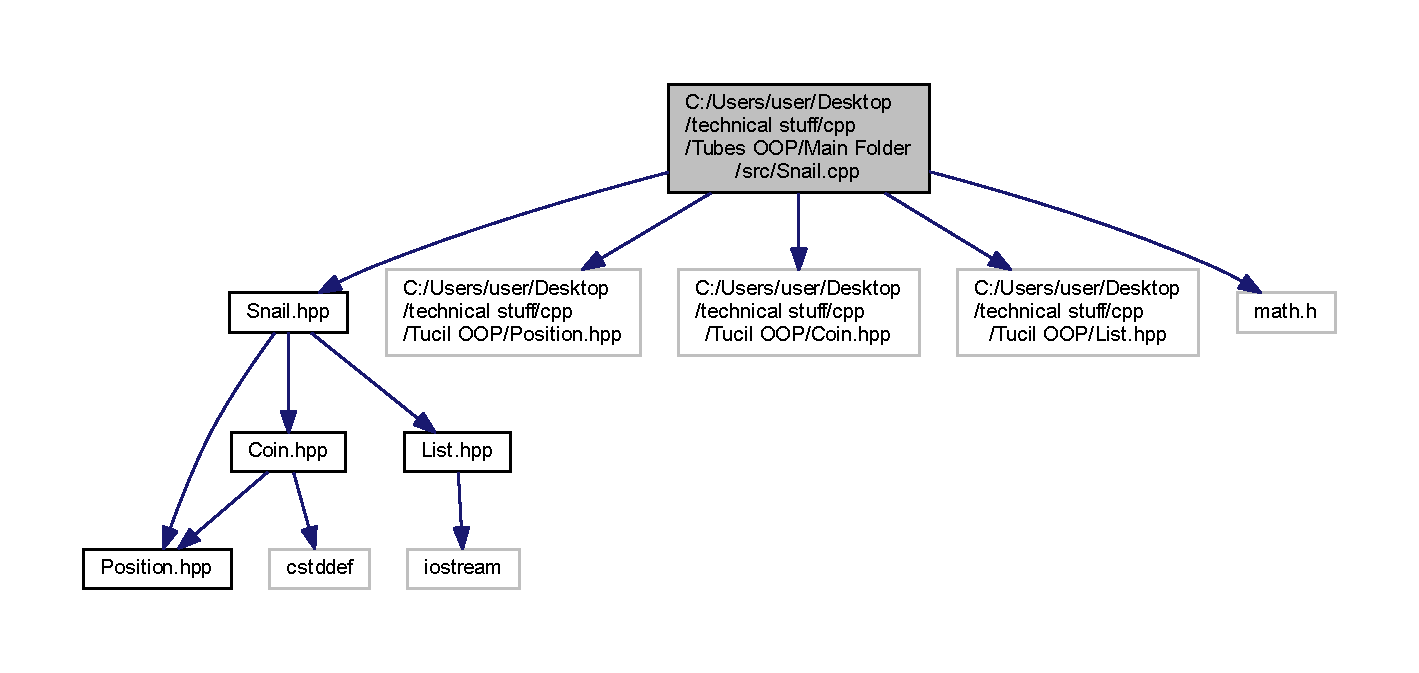
\includegraphics[width=350pt]{_snail_8cpp__incl}
\end{center}
\end{figure}

\hypertarget{main__coin_8cpp}{}\section{C\+:/\+Users/user/\+Desktop/technical stuff/cpp/\+Tubes O\+O\+P/\+Main Folder/test\+\_\+driver/\+Coin/main\+\_\+coin.cpp File Reference}
\label{main__coin_8cpp}\index{C\+:/\+Users/user/\+Desktop/technical stuff/cpp/\+Tubes O\+O\+P/\+Main Folder/test\+\_\+driver/\+Coin/main\+\_\+coin.\+cpp@{C\+:/\+Users/user/\+Desktop/technical stuff/cpp/\+Tubes O\+O\+P/\+Main Folder/test\+\_\+driver/\+Coin/main\+\_\+coin.\+cpp}}
{\ttfamily \#include \char`\"{}Coin.\+hpp\char`\"{}}\newline
{\ttfamily \#include $<$iostream$>$}\newline
Include dependency graph for main\+\_\+coin.\+cpp\+:
\nopagebreak
\begin{figure}[H]
\begin{center}
\leavevmode
\includegraphics[width=255pt]{main__coin_8cpp__incl}
\end{center}
\end{figure}
\subsection*{Functions}
\begin{DoxyCompactItemize}
\item 
int \mbox{\hyperlink{main__coin_8cpp_ae66f6b31b5ad750f1fe042a706a4e3d4}{main}} ()
\end{DoxyCompactItemize}


\subsection{Function Documentation}
\mbox{\Hypertarget{main__coin_8cpp_ae66f6b31b5ad750f1fe042a706a4e3d4}\label{main__coin_8cpp_ae66f6b31b5ad750f1fe042a706a4e3d4}} 
\index{main\+\_\+coin.\+cpp@{main\+\_\+coin.\+cpp}!main@{main}}
\index{main@{main}!main\+\_\+coin.\+cpp@{main\+\_\+coin.\+cpp}}
\subsubsection{\texorpdfstring{main()}{main()}}
{\footnotesize\ttfamily int main (\begin{DoxyParamCaption}{ }\end{DoxyParamCaption})}


\hypertarget{main__guppy_8cpp}{}\section{C\+:/\+Users/user/\+Desktop/technical stuff/cpp/\+Tubes O\+O\+P/\+Main Folder/test\+\_\+driver/\+Ikan/main\+\_\+guppy.cpp File Reference}
\label{main__guppy_8cpp}\index{C\+:/\+Users/user/\+Desktop/technical stuff/cpp/\+Tubes O\+O\+P/\+Main Folder/test\+\_\+driver/\+Ikan/main\+\_\+guppy.\+cpp@{C\+:/\+Users/user/\+Desktop/technical stuff/cpp/\+Tubes O\+O\+P/\+Main Folder/test\+\_\+driver/\+Ikan/main\+\_\+guppy.\+cpp}}
{\ttfamily \#include \char`\"{}Ikan.\+hpp\char`\"{}}\newline
{\ttfamily \#include $<$stdlib.\+h$>$}\newline
{\ttfamily \#include $<$time.\+h$>$}\newline
{\ttfamily \#include $<$stdio.\+h$>$}\newline
{\ttfamily \#include $<$iostream$>$}\newline
Include dependency graph for main\+\_\+guppy.\+cpp\+:
\nopagebreak
\begin{figure}[H]
\begin{center}
\leavevmode
\includegraphics[width=350pt]{main__guppy_8cpp__incl}
\end{center}
\end{figure}
\subsection*{Functions}
\begin{DoxyCompactItemize}
\item 
int \mbox{\hyperlink{main__guppy_8cpp_ae66f6b31b5ad750f1fe042a706a4e3d4}{main}} ()
\end{DoxyCompactItemize}


\subsection{Function Documentation}
\mbox{\Hypertarget{main__guppy_8cpp_ae66f6b31b5ad750f1fe042a706a4e3d4}\label{main__guppy_8cpp_ae66f6b31b5ad750f1fe042a706a4e3d4}} 
\index{main\+\_\+guppy.\+cpp@{main\+\_\+guppy.\+cpp}!main@{main}}
\index{main@{main}!main\+\_\+guppy.\+cpp@{main\+\_\+guppy.\+cpp}}
\subsubsection{\texorpdfstring{main()}{main()}}
{\footnotesize\ttfamily int main (\begin{DoxyParamCaption}{ }\end{DoxyParamCaption})}


\hypertarget{main__list_8cpp}{}\section{C\+:/\+Users/user/\+Desktop/technical stuff/cpp/\+Tubes O\+O\+P/\+Main Folder/test\+\_\+driver/\+List/main\+\_\+list.cpp File Reference}
\label{main__list_8cpp}\index{C\+:/\+Users/user/\+Desktop/technical stuff/cpp/\+Tubes O\+O\+P/\+Main Folder/test\+\_\+driver/\+List/main\+\_\+list.\+cpp@{C\+:/\+Users/user/\+Desktop/technical stuff/cpp/\+Tubes O\+O\+P/\+Main Folder/test\+\_\+driver/\+List/main\+\_\+list.\+cpp}}
{\ttfamily \#include \char`\"{}List.\+hpp\char`\"{}}\newline
{\ttfamily \#include \char`\"{}Guppy.\+hpp\char`\"{}}\newline
{\ttfamily \#include $<$iostream$>$}\newline
Include dependency graph for main\+\_\+list.\+cpp\+:
\nopagebreak
\begin{figure}[H]
\begin{center}
\leavevmode
\includegraphics[width=350pt]{main__list_8cpp__incl}
\end{center}
\end{figure}
\subsection*{Functions}
\begin{DoxyCompactItemize}
\item 
int \mbox{\hyperlink{main__list_8cpp_ae66f6b31b5ad750f1fe042a706a4e3d4}{main}} ()
\end{DoxyCompactItemize}


\subsection{Function Documentation}
\mbox{\Hypertarget{main__list_8cpp_ae66f6b31b5ad750f1fe042a706a4e3d4}\label{main__list_8cpp_ae66f6b31b5ad750f1fe042a706a4e3d4}} 
\index{main\+\_\+list.\+cpp@{main\+\_\+list.\+cpp}!main@{main}}
\index{main@{main}!main\+\_\+list.\+cpp@{main\+\_\+list.\+cpp}}
\subsubsection{\texorpdfstring{main()}{main()}}
{\footnotesize\ttfamily int main (\begin{DoxyParamCaption}{ }\end{DoxyParamCaption})}


\hypertarget{main__makanan_8cpp}{}\section{C\+:/\+Users/user/\+Desktop/technical stuff/cpp/\+Tubes O\+O\+P/\+Main Folder/test\+\_\+driver/\+Makanan/main\+\_\+makanan.cpp File Reference}
\label{main__makanan_8cpp}\index{C\+:/\+Users/user/\+Desktop/technical stuff/cpp/\+Tubes O\+O\+P/\+Main Folder/test\+\_\+driver/\+Makanan/main\+\_\+makanan.\+cpp@{C\+:/\+Users/user/\+Desktop/technical stuff/cpp/\+Tubes O\+O\+P/\+Main Folder/test\+\_\+driver/\+Makanan/main\+\_\+makanan.\+cpp}}
{\ttfamily \#include \char`\"{}Makanan.\+hpp\char`\"{}}\newline
{\ttfamily \#include $<$stdlib.\+h$>$}\newline
{\ttfamily \#include $<$iostream$>$}\newline
Include dependency graph for main\+\_\+makanan.\+cpp\+:
\nopagebreak
\begin{figure}[H]
\begin{center}
\leavevmode
\includegraphics[width=325pt]{main__makanan_8cpp__incl}
\end{center}
\end{figure}
\subsection*{Functions}
\begin{DoxyCompactItemize}
\item 
int \mbox{\hyperlink{main__makanan_8cpp_ae66f6b31b5ad750f1fe042a706a4e3d4}{main}} ()
\end{DoxyCompactItemize}


\subsection{Function Documentation}
\mbox{\Hypertarget{main__makanan_8cpp_ae66f6b31b5ad750f1fe042a706a4e3d4}\label{main__makanan_8cpp_ae66f6b31b5ad750f1fe042a706a4e3d4}} 
\index{main\+\_\+makanan.\+cpp@{main\+\_\+makanan.\+cpp}!main@{main}}
\index{main@{main}!main\+\_\+makanan.\+cpp@{main\+\_\+makanan.\+cpp}}
\subsubsection{\texorpdfstring{main()}{main()}}
{\footnotesize\ttfamily int main (\begin{DoxyParamCaption}{ }\end{DoxyParamCaption})}


\hypertarget{_piranha__test_8cpp}{}\section{test\+\_\+driver/\+Piranha/\+Piranha\+\_\+test.cpp File Reference}
\label{_piranha__test_8cpp}\index{test\+\_\+driver/\+Piranha/\+Piranha\+\_\+test.\+cpp@{test\+\_\+driver/\+Piranha/\+Piranha\+\_\+test.\+cpp}}
{\ttfamily \#include \char`\"{}Piranha.\+hpp\char`\"{}}\newline
{\ttfamily \#include $<$stdlib.\+h$>$}\newline
{\ttfamily \#include $<$iostream$>$}\newline
Include dependency graph for Piranha\+\_\+test.\+cpp\+:
\nopagebreak
\begin{figure}[H]
\begin{center}
\leavevmode
\includegraphics[width=350pt]{_piranha__test_8cpp__incl}
\end{center}
\end{figure}
\subsection*{Functions}
\begin{DoxyCompactItemize}
\item 
int \mbox{\hyperlink{_piranha__test_8cpp_ae66f6b31b5ad750f1fe042a706a4e3d4}{main}} ()
\end{DoxyCompactItemize}


\subsection{Function Documentation}
\mbox{\Hypertarget{_piranha__test_8cpp_ae66f6b31b5ad750f1fe042a706a4e3d4}\label{_piranha__test_8cpp_ae66f6b31b5ad750f1fe042a706a4e3d4}} 
\index{Piranha\+\_\+test.\+cpp@{Piranha\+\_\+test.\+cpp}!main@{main}}
\index{main@{main}!Piranha\+\_\+test.\+cpp@{Piranha\+\_\+test.\+cpp}}
\subsubsection{\texorpdfstring{main()}{main()}}
{\footnotesize\ttfamily int main (\begin{DoxyParamCaption}{ }\end{DoxyParamCaption})}


\hypertarget{main__position_8cpp}{}\section{test\+\_\+driver/\+Position/main\+\_\+position.cpp File Reference}
\label{main__position_8cpp}\index{test\+\_\+driver/\+Position/main\+\_\+position.\+cpp@{test\+\_\+driver/\+Position/main\+\_\+position.\+cpp}}
{\ttfamily \#include \char`\"{}Position.\+hpp\char`\"{}}\newline
{\ttfamily \#include $<$iostream$>$}\newline
Include dependency graph for main\+\_\+position.\+cpp\+:
\nopagebreak
\begin{figure}[H]
\begin{center}
\leavevmode
\includegraphics[width=224pt]{main__position_8cpp__incl}
\end{center}
\end{figure}
\subsection*{Functions}
\begin{DoxyCompactItemize}
\item 
int \mbox{\hyperlink{main__position_8cpp_ae66f6b31b5ad750f1fe042a706a4e3d4}{main}} ()
\end{DoxyCompactItemize}


\subsection{Function Documentation}
\mbox{\Hypertarget{main__position_8cpp_ae66f6b31b5ad750f1fe042a706a4e3d4}\label{main__position_8cpp_ae66f6b31b5ad750f1fe042a706a4e3d4}} 
\index{main\+\_\+position.\+cpp@{main\+\_\+position.\+cpp}!main@{main}}
\index{main@{main}!main\+\_\+position.\+cpp@{main\+\_\+position.\+cpp}}
\subsubsection{\texorpdfstring{main()}{main()}}
{\footnotesize\ttfamily int main (\begin{DoxyParamCaption}{ }\end{DoxyParamCaption})}


%--- End generated contents ---

% Index
\backmatter
\newpage
\phantomsection
\clearemptydoublepage
\addcontentsline{toc}{chapter}{Index}
\printindex

\end{document}
